\documentclass[]{article}
\usepackage{lmodern}
\usepackage{amssymb,amsmath}
\usepackage{ifxetex,ifluatex}
\usepackage{fixltx2e} % provides \textsubscript
\ifnum 0\ifxetex 1\fi\ifluatex 1\fi=0 % if pdftex
  \usepackage[T1]{fontenc}
  \usepackage[utf8]{inputenc}
\else % if luatex or xelatex
  \ifxetex
    \usepackage{mathspec}
  \else
    \usepackage{fontspec}
  \fi
  \defaultfontfeatures{Ligatures=TeX,Scale=MatchLowercase}
\fi
% use upquote if available, for straight quotes in verbatim environments
\IfFileExists{upquote.sty}{\usepackage{upquote}}{}
% use microtype if available
\IfFileExists{microtype.sty}{%
\usepackage{microtype}
\UseMicrotypeSet[protrusion]{basicmath} % disable protrusion for tt fonts
}{}
\usepackage[margin=1in]{geometry}
\usepackage{hyperref}
\hypersetup{unicode=true,
            pdftitle={All Women Shortlists Methodology},
            pdfauthor={Evan Odell},
            pdfborder={0 0 0},
            breaklinks=true}
\urlstyle{same}  % don't use monospace font for urls
\usepackage{longtable,booktabs}
\usepackage{graphicx,grffile}
\makeatletter
\def\maxwidth{\ifdim\Gin@nat@width>\linewidth\linewidth\else\Gin@nat@width\fi}
\def\maxheight{\ifdim\Gin@nat@height>\textheight\textheight\else\Gin@nat@height\fi}
\makeatother
% Scale images if necessary, so that they will not overflow the page
% margins by default, and it is still possible to overwrite the defaults
% using explicit options in \includegraphics[width, height, ...]{}
\setkeys{Gin}{width=\maxwidth,height=\maxheight,keepaspectratio}
\IfFileExists{parskip.sty}{%
\usepackage{parskip}
}{% else
\setlength{\parindent}{0pt}
\setlength{\parskip}{6pt plus 2pt minus 1pt}
}
\setlength{\emergencystretch}{3em}  % prevent overfull lines
\providecommand{\tightlist}{%
  \setlength{\itemsep}{0pt}\setlength{\parskip}{0pt}}
\setcounter{secnumdepth}{5}
% Redefines (sub)paragraphs to behave more like sections
\ifx\paragraph\undefined\else
\let\oldparagraph\paragraph
\renewcommand{\paragraph}[1]{\oldparagraph{#1}\mbox{}}
\fi
\ifx\subparagraph\undefined\else
\let\oldsubparagraph\subparagraph
\renewcommand{\subparagraph}[1]{\oldsubparagraph{#1}\mbox{}}
\fi

%%% Use protect on footnotes to avoid problems with footnotes in titles
\let\rmarkdownfootnote\footnote%
\def\footnote{\protect\rmarkdownfootnote}

%%% Change title format to be more compact
\usepackage{titling}

% Create subtitle command for use in maketitle
\newcommand{\subtitle}[1]{
  \posttitle{
    \begin{center}\large#1\end{center}
    }
}

\setlength{\droptitle}{-2em}

  \title{All Women Shortlists Methodology}
    \pretitle{\vspace{\droptitle}\centering\huge}
  \posttitle{\par}
    \author{Evan Odell}
    \preauthor{\centering\large\emph}
  \postauthor{\par}
      \predate{\centering\large\emph}
  \postdate{\par}
    \date{2018-10-25}

\usepackage{array}
\usepackage{float}
\let\origfigure\figure
\let\endorigfigure\endfigure
\renewenvironment{figure}[1][2] {
    \expandafter\origfigure\expandafter[H]
} {
    \endorigfigure
}
\usepackage{booktabs}
\usepackage{longtable}
\usepackage{array}
\usepackage{multirow}
\usepackage[table]{xcolor}
\usepackage{wrapfig}
\usepackage{float}
\usepackage{colortbl}
\usepackage{pdflscape}
\usepackage{tabu}
\usepackage{threeparttable}
\usepackage{threeparttablex}
\usepackage[normalem]{ulem}
\usepackage{makecell}

\usepackage{amsthm}
\newtheorem{theorem}{Theorem}[section]
\newtheorem{lemma}{Lemma}[section]
\theoremstyle{definition}
\newtheorem{definition}{Definition}[section]
\newtheorem{corollary}{Corollary}[section]
\newtheorem{proposition}{Proposition}[section]
\theoremstyle{definition}
\newtheorem{example}{Example}[section]
\theoremstyle{definition}
\newtheorem{exercise}{Exercise}[section]
\theoremstyle{remark}
\newtheorem*{remark}{Remark}
\newtheorem*{solution}{Solution}
\begin{document}
\maketitle

{
\setcounter{tocdepth}{3}
\tableofcontents
}
\listoftables
\listoffigures
\clearpage

\hypertarget{descriptive-statistics}{%
\section{Descriptive Statistics}\label{descriptive-statistics}}

Table \ref{tab:lab-desc-stats-table} shows the number of Labour MPs
elected in each general election from 1997 to 2015, including newly
elected MPs (the ``intake''), the number of newly elected MPs from all
women shortlists (AWS), and the number of candidates selected through
all women shortlists. Data in Table \ref{tab:lab-desc-stats-table} is
from the House of Commons Library (Audickas, Hawkins, \& Cracknell,
\protect\hyperlink{ref-audickas2017}{2017}; Kelly \& White,
\protect\hyperlink{ref-kelly2016}{2016}). All women shortlists were not
used by Labour during the 2001 General Election.

\begin{table}[H]

\caption{\label{tab:lab-desc-stats-table}Labour MPs and Intakes}
\centering
\begin{tabular}[t]{>{\raggedleft\arraybackslash}p{1.5cm}>{\raggedleft\arraybackslash}p{1cm}>{\raggedleft\arraybackslash}p{1.5cm}>{\raggedleft\arraybackslash}p{2cm}>{\raggedleft\arraybackslash}p{2cm}>{\raggedleft\arraybackslash}p{1.5cm}>{\raggedleft\arraybackslash}p{1.5cm}>{\raggedleft\arraybackslash}p{2cm}}
\toprule
General Election & Total MPs & Labour MPs & Female Labour MPs & Labour MPs Intake & Intake Women & Intake Shortlist & Nominated Shortlist\\
\midrule
1997 & 659 & 418 & 101 (24\%) & 177 & 64 (36\%) & 35 & 38\\
2001 & 659 & 412 & 95 (23\%) & 38 & 4 (11\%) & 0 & 0\\
2005 & 646 & 355 & 98 (28\%) & 40 & 26 (65\%) & 23 & 30\\
2010 & 650 & 258 & 81 (31\%) & 64 & 32 (50\%) & 28 & 63\\
2015 & 650 & 232 & 99 (43\%) & 49 & 31 (63\%) & 31 & 77\\
\bottomrule
\end{tabular}
\end{table}

Table \ref{tab:speech-stats-table} shows the total size of the dataset
in speeches and words by each party, including by gender for each party,
and in the case of female Labour MPs, by AWS status. Details on
inclusion criteria are given \protect\hyperlink{methodology}{below}.

\begin{table}[H]

\caption{\label{tab:speech-stats-table}Number of Speeches and Words in Dataset}
\centering
\begin{tabular}[t]{lrr}
\toprule
Gender & Speeches & Words\\
\midrule
All & 657,547 & 239,123,685\\
Female & 149,805 & 56,589,501\\
Male & 507,742 & 182,534,184\\
\addlinespace[0.3em]
\multicolumn{3}{l}{\textbf{Conservatives}}\\
\hspace{1em}All & 285,308 & 96,186,824\\
\hspace{1em}Female & 48,771 & 15,779,116\\
\hspace{1em}Male & 236,537 & 80,407,708\\
\addlinespace[0.3em]
\multicolumn{3}{l}{\textbf{Labour}}\\
\hspace{1em}All & 262,000 & 99,986,437\\
\hspace{1em}Female & 84,615 & 34,159,304\\
\hspace{1em}\hspace{1em}Non-All Women Shortlists & 28,653 & 11,623,184\\
\hspace{1em}\hspace{1em}All Women Shortlists & 55,962 & 22,536,120\\
\hspace{1em}Male & 177,385 & 65,827,133\\
\addlinespace[0.3em]
\multicolumn{3}{l}{\textbf{Liberal Democrat}}\\
\hspace{1em}All & 72,719 & 28,947,968\\
\hspace{1em}Female & 7,552 & 3,232,822\\
\hspace{1em}Male & 65,167 & 25,715,146\\
\addlinespace[0.3em]
\multicolumn{3}{l}{\textbf{Other}}\\
\hspace{1em}All & 37,520 & 14,002,456\\
\hspace{1em}Female & 8,867 & 3,418,259\\
\hspace{1em}Male & 28,653 & 10,584,197\\
\bottomrule
\end{tabular}
\end{table}

\hypertarget{methodology}{%
\section{Methodology}\label{methodology}}

Previous research on gender differences in political speech patterns has
focused on differences between male and female politicians (Yu,
\protect\hyperlink{ref-yu2014}{2014}) or on variations in Hilary
Clinton's speech patterns (Bligh, Merolla, Schroedel, \& Gonzalez,
\protect\hyperlink{ref-bligh2010}{2010}; Jones,
\protect\hyperlink{ref-jones2016}{2016}). This paper focuses on
differences in speech patterns between female Labour MPs nominated
through All Women Shortlists (AWS) and female Labour MPs nominated
through open shortlists. We examined differences in speaking styles
using the \texttt{Linguistic\ Inquiry\ and\ Word\ Count\ 2015} (LIWC)
dictionary (Pennebaker, Boyd, Jordan, \& Blackburn,
\protect\hyperlink{ref-pennebaker2015}{2015}) and the \texttt{spaCy}
(Honnibal \& Montani, \protect\hyperlink{ref-honnibal2017}{2017})
Parts-of-Speech (POS) tagger. We examined differences in the topics
discussed by AWS and non-AWS MPs, using \({\chi}^2\) tests for
individual words and for bigrams. We trained a Naive Bayes classifier to
distinguish AWS and non-AWS speeches. We used structured topic models
(STM) to identify the topics discussed by AWS and non-AWS MPs.

To account for the possible effects of age, parliamentary experience and
cohort, and in order to compare women selected through all women
shortlists to women who were not (but who theoretically had the
opportunity to contest all-women shortlists), our analysis is been
restricted only to Labour MPs first elected to the House of Commons in
the 1997 General Election, up to but excluding the 2017 General
Election. Comparisons between MPs of different parties are also
restricted to MPs first elected in the 1997 General Election, and before
the 2017 General Election. Speeches made by the Speaker, including
Deputy Speakers, were also excluded. Words contained in parentheses were
removed, as they are added by Hansard to provide additional information
not actually spoken by the MP.\footnote{e.g.~a reference to ``the member
  for Bethnal Green and Bow'' in keeping with Parliamentary convention
  of identifying MPs by their seat rather than their name would be
  followed by ``(Rushnara Ali)''.} Speeches and data on MPs' gender and
party affiliation are from a previously assembled dataset (Odell,
\protect\hyperlink{ref-odell2018}{2018}). Information on candidates
selected through all women shortlists is from the House of Commons
Library (Kelly \& White, \protect\hyperlink{ref-kelly2016}{2016}).
Unsuccessful General Election candidates selected through all women
shortlists who were subsequently elected in a byelection are classified
as having been selected on an all women shortlist, regardless of the
selection process for that byelection. Speeches made by MPs while
suspended from the Labour party where classified the same as if they had
not been suspended. The dataset includes 408 different Labour MPs, 167
female MPs, 119 elected from All Women Shortlists and 48 elected from
open shortlists, along with 241 male MPs.

\hypertarget{results}{%
\section{Results}\label{results}}

\hypertarget{linguistic-inquiry-and-word-count}{%
\subsection{Linguistic Inquiry and Word
Count}\label{linguistic-inquiry-and-word-count}}

Word classification used the
\texttt{Linguistic\ Inquiry\ and\ Word\ Count\ 2015} (LIWC) dictionary
(Pennebaker et al., \protect\hyperlink{ref-pennebaker2015}{2015}) and
tokenising tools from the \texttt{Quanteda} \texttt{R} package (Benoit,
\protect\hyperlink{ref-benoit2018}{2018}). Word counts and
words-per-sentence, and calculations for determining grade level
(Kincaid, Fishburne, Rogers, \& Chissom,
\protect\hyperlink{ref-kincaid1975}{1975}) were produced using
\texttt{stringi} (Gagolewski,
\protect\hyperlink{ref-gagolewski2018}{2018}), an \texttt{R} wrapper to
the ICU regex library.

Following research by Yu (\protect\hyperlink{ref-yu2014}{2014}) and
Newman, Groom, Handelman, \& Pennebaker
(\protect\hyperlink{ref-newman2008}{2008}) on gender differences in
language, we focused on the following LIWC categories to compare MPs'
speeches:

\begin{itemize}
\tightlist
\item
  All Pronouns (pronoun)
\item
  First person singular pronouns (i) 
\item
  First person plural pronouns (we)
\item
  Verbs (verb)
\item
  Auxiliary verbs (auxverb) 
\item
  Social processes (social) 
\item
  Positive emotions (posemo) 
\item
  Negative emotions (negemo) 
\item
  Tentative words (tentat)
\item
  Articles (article) 
\item
  Prepositions (preps) 
\item
  Anger words (anger)
\item
  Swear words (swear)
\item
  Cognitive processes (cogproc)
\item
  Words longer than six letters (Sixltr)
\end{itemize}

We also included mean words-per-sentence (WPS), total speach word count
(WC) and Flesch--Kincaid grade level (FK) (Kincaid et al.,
\protect\hyperlink{ref-kincaid1975}{1975}), calculated using the
\texttt{Quanteda} (Benoit, \protect\hyperlink{ref-benoit2018}{2018}) and
\texttt{stringi} (Gagolewski,
\protect\hyperlink{ref-gagolewski2018}{2018}) \texttt{R} packages.

\hypertarget{women-vs-men}{%
\subsubsection{Women vs Men}\label{women-vs-men}}

Table \ref{tab:gender-effect-sizes-table} shows there are no categories
where gender differences meet the effect size threshold of \(|0.2|\)
suggested by Cohen (\protect\hyperlink{ref-cohen1988}{1988}, pp. 25--26)
to indicate a small effect. 4 categories -- words with more than six
letters, prepositions, words-per-sentence and Flesh-Kincaid grade level
-- met or exceeded the \(|0.1|\) threshold suggested by Newman et al.
(\protect\hyperlink{ref-newman2008}{2008}).

\begin{table}[H]

\caption{\label{tab:gender-effect-sizes-table}Effect Sizes for Male and Female Labour MPs}
\centering
\begin{tabular}[t]{lrrrrrl}
\toprule
\multicolumn{1}{c}{ } & \multicolumn{2}{c}{Women} & \multicolumn{2}{c}{Men} & \multicolumn{2}{c}{Effect Size} \\
\cmidrule(l{2pt}r{2pt}){2-3} \cmidrule(l{2pt}r{2pt}){4-5} \cmidrule(l{2pt}r{2pt}){6-7}
 & Mean & SD & Mean & SD & Cohen's d & Magnitude\\
\midrule
All Pronouns & 10.07 & 4.60 & 10.15 & 4.99 & 0.02 & negligible\\
First person singular pronouns & 1.89 & 2.41 & 2.02 & 2.55 & 0.05 & negligible\\
First person plural pronouns & 0.98 & 1.42 & 0.99 & 1.51 & 0.01 & negligible\\
Verbs & 12.82 & 5.00 & 12.67 & 5.35 & -0.03 & negligible\\
Auxiliary verbs & 7.91 & 3.45 & 7.93 & 3.69 & 0.01 & negligible\\
\addlinespace
Social processes & 8.46 & 4.81 & 8.16 & 5.11 & -0.06 & negligible\\
Positive emotions & 2.73 & 2.49 & 2.57 & 2.54 & -0.06 & negligible\\
Negative emotions & 1.15 & 1.69 & 1.07 & 1.78 & -0.05 & negligible\\
Tentative words & 1.48 & 1.74 & 1.58 & 1.90 & 0.05 & negligible\\
More than six letters & 10.62 & 3.67 & 10.26 & 3.92 & -0.10 & negligible\\
\addlinespace
Articles & 7.64 & 3.30 & 7.96 & 3.55 & 0.09 & negligible\\
Prepositions & 12.58 & 4.41 & 12.14 & 4.73 & -0.10 & negligible\\
Anger words & 0.23 & 0.83 & 0.24 & 0.79 & 0.01 & negligible\\
Swear words & 0.00 & 0.06 & 0.00 & 0.09 & 0.01 & negligible\\
Cognitive processes & 8.68 & 4.83 & 8.82 & 5.15 & 0.03 & negligible\\
\addlinespace
Words per Sentence & 43.99 & 19.92 & 41.43 & 20.30 & -0.13 & negligible\\
Total Word Count & 402.72 & 691.10 & 370.13 & 647.25 & -0.05 & negligible\\
Flesh-Kincaid Grade Level & 10.97 & 7.77 & 9.91 & 7.96 & -0.13 & negligible\\
\bottomrule
\end{tabular}
\end{table}

\hypertarget{shortlists-vs-non-shortlists}{%
\subsubsection{Shortlists vs
Non-Shortlists}\label{shortlists-vs-non-shortlists}}

Figure \ref{fig:sl-key-y-since-start} shows changes in the occurrences
of selected LIWC terms, words-per-sentence, total word count and
Flesch--Kincaid grade level, over the course of an MP's career, as
measured since the time an MP was first elected. There do not appear to
be any notable changes in speaking style over the course of female
Labour MPs' careers. Figure \ref{fig:sl-key-date} shows changes in the
occurrences of the same selected terms from 1997--2017. As in Figure
\ref{fig:sl-key-y-since-start}, there do not appear to be any meaningful
trends in the use of the selected terms over time.

There are no categories among female Labour MPs by selection process
meeting the \(|0.2|\) threshold, as shown in Table
\ref{tab:sl-effect-sizes}. Only one category - first person plural
pronouns, \emph{d}=0.19 -- exceeded \(|0.1|\).

\begin{figure}
\centering
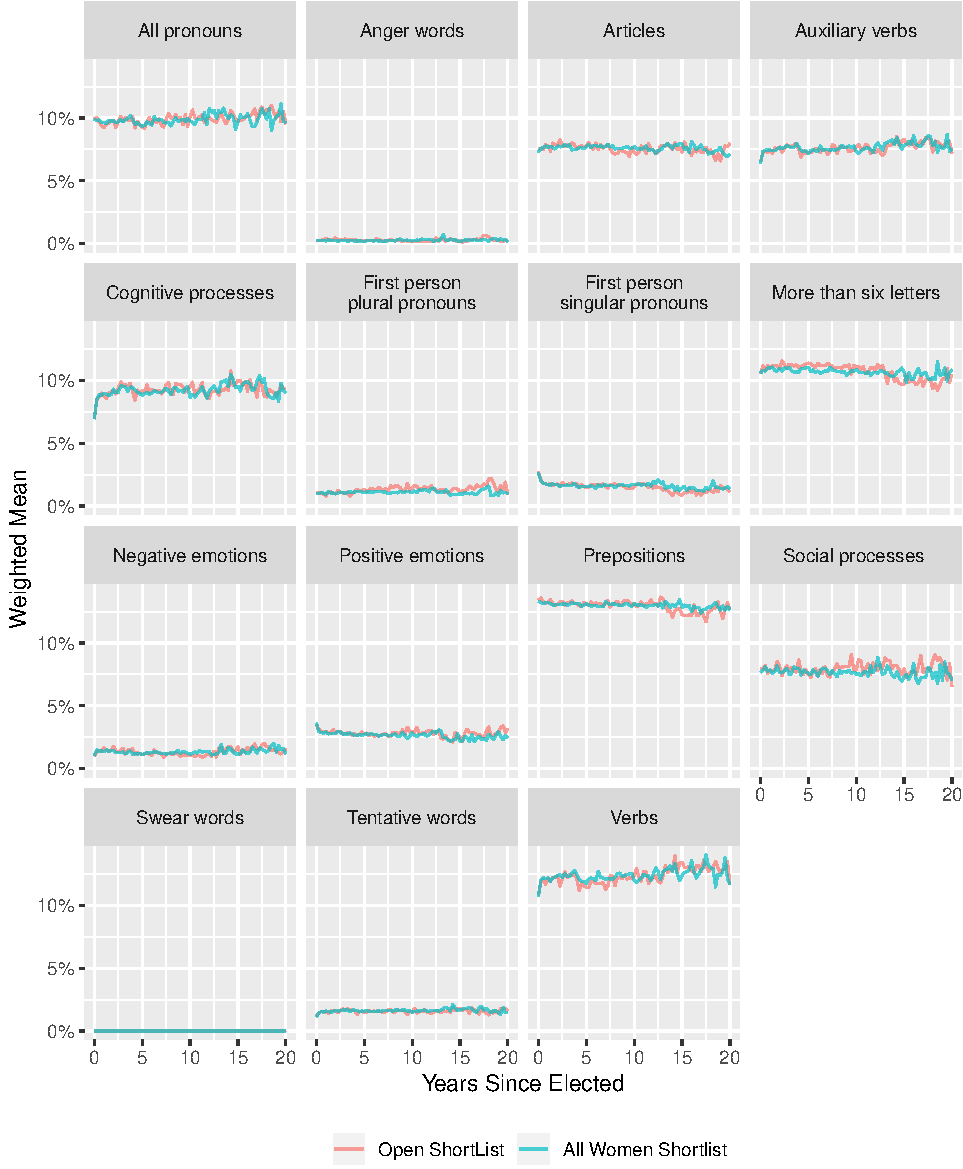
\includegraphics{methodology_files/figure-latex/sl-key-y-since-start-1.pdf}
\caption{\label{fig:sl-key-y-since-start}Occurrence of selected LIWC terms,
by time as MP}
\end{figure}

\begin{figure}
\centering
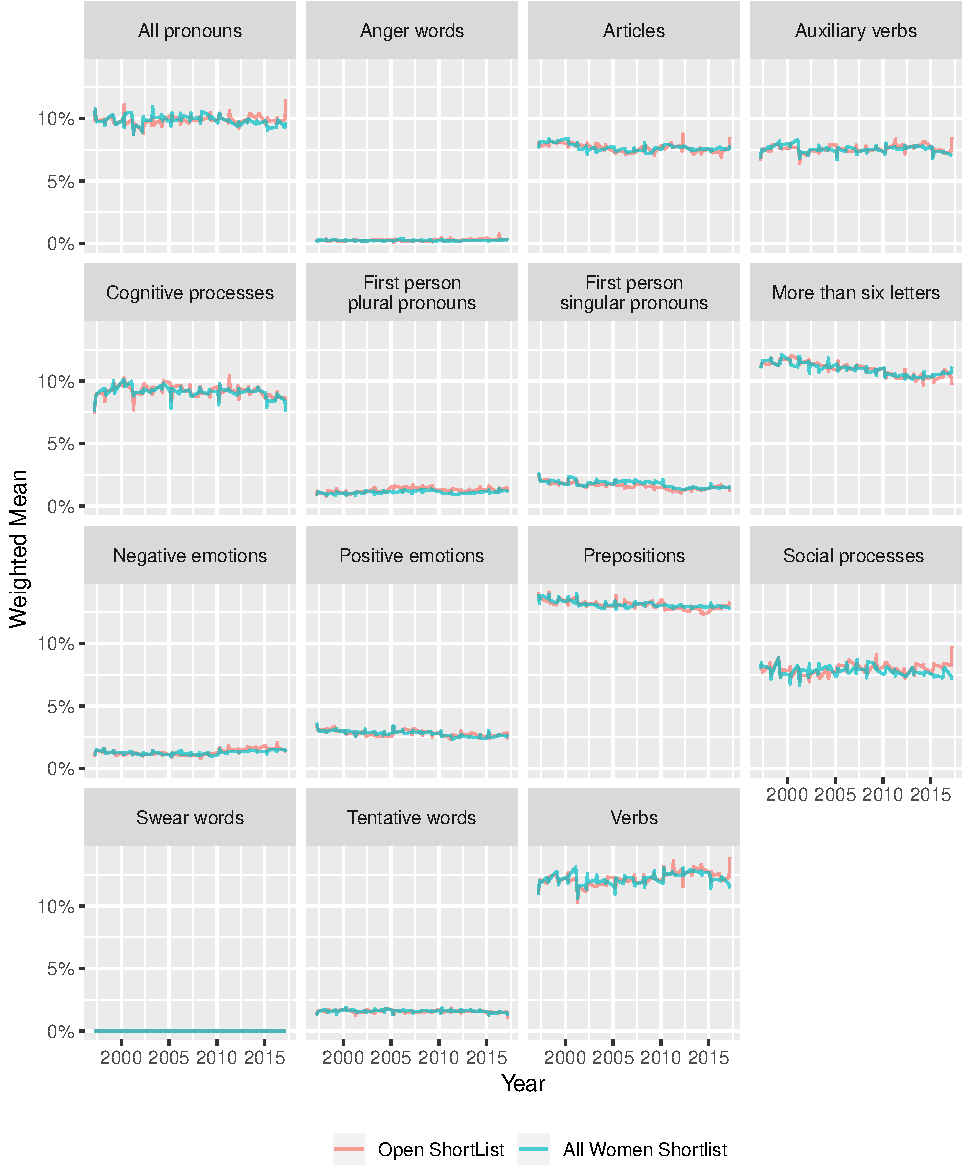
\includegraphics{methodology_files/figure-latex/sl-key-date-1.pdf}
\caption{\label{fig:sl-key-date}Occurrence of selected LIWC terms, by date}
\end{figure}

\begin{table}[H]

\caption{\label{tab:sl-effect-sizes}Effect Sizes for Female Labour MPs by selection process}
\centering
\begin{tabular}[t]{lrrrrrl}
\toprule
\multicolumn{1}{c}{ } & \multicolumn{2}{c}{All Women Shortlists} & \multicolumn{2}{c}{Open Shortlists} & \multicolumn{2}{c}{Effect Size} \\
\cmidrule(l{2pt}r{2pt}){2-3} \cmidrule(l{2pt}r{2pt}){4-5} \cmidrule(l{2pt}r{2pt}){6-7}
 & Mean & SD & Mean & SD & Cohen's d & Magnitude\\
\midrule
All Pronouns & 10.01 & 4.66 & 10.19 & 4.47 & -0.04 & negligible\\
First person singular pronouns & 1.86 & 2.41 & 1.95 & 2.42 & -0.04 & negligible\\
First person plural pronouns & 0.88 & 1.36 & 1.16 & 1.51 & -0.19 & negligible\\
Verbs & 12.88 & 5.10 & 12.69 & 4.80 & 0.04 & negligible\\
Auxiliary verbs & 7.94 & 3.49 & 7.86 & 3.38 & 0.02 & negligible\\
\addlinespace
Social processes & 8.46 & 4.93 & 8.44 & 4.58 & 0.00 & negligible\\
Positive emotions & 2.69 & 2.52 & 2.81 & 2.42 & -0.05 & negligible\\
Negative emotions & 1.17 & 1.69 & 1.13 & 1.68 & 0.02 & negligible\\
Tentative words & 1.48 & 1.75 & 1.49 & 1.73 & 0.00 & negligible\\
More than six letters & 10.56 & 3.72 & 10.74 & 3.56 & -0.05 & negligible\\
\addlinespace
Articles & 7.69 & 3.38 & 7.55 & 3.14 & 0.04 & negligible\\
Prepositions & 12.55 & 4.54 & 12.63 & 4.14 & -0.02 & negligible\\
Anger words & 0.23 & 0.79 & 0.24 & 0.91 & -0.01 & negligible\\
Swear words & 0.00 & 0.06 & 0.00 & 0.05 & 0.01 & negligible\\
Cognitive processes & 8.59 & 4.90 & 8.85 & 4.69 & -0.05 & negligible\\
\addlinespace
Words per Sentence & 44.39 & 20.69 & 43.21 & 18.31 & 0.06 & negligible\\
Total Word Count & 401.70 & 704.15 & 404.73 & 664.87 & 0.00 & negligible\\
Flesh-Kincaid Grade Level & 11.13 & 8.06 & 10.64 & 7.15 & 0.07 & negligible\\
\bottomrule
\end{tabular}
\end{table}

\hypertarget{conservatives-vs-labour}{%
\subsubsection{Conservatives vs Labour}\label{conservatives-vs-labour}}

As shown in Table \ref{tab:tory-labour-effect-sizes-table}, there are no
categories with effect sizes exceeding \(|0.2|\) between Labour and
Conservative MPs, and only one (first person plural pronouns) exceeding
\(|0.1|\).

\begin{table}[H]

\caption{\label{tab:tory-labour-effect-sizes-table}Effect Sizes for All Labour and Conservative MPs}
\centering
\begin{tabular}[t]{lrrrrrl}
\toprule
\multicolumn{1}{c}{ } & \multicolumn{2}{c}{Labour} & \multicolumn{2}{c}{Conservatives} & \multicolumn{2}{c}{Effect Size} \\
\cmidrule(l{2pt}r{2pt}){2-3} \cmidrule(l{2pt}r{2pt}){4-5} \cmidrule(l{2pt}r{2pt}){6-7}
 & Mean & SD & Mean & SD & Cohen's d & Magnitude\\
\midrule
All Pronouns & 10.12 & 4.87 & 10.61 & 4.84 & 0.10 & negligible\\
First person singular pronouns & 1.98 & 2.51 & 2.14 & 2.56 & 0.06 & negligible\\
First person plural pronouns & 0.98 & 1.48 & 1.22 & 1.70 & 0.15 & negligible\\
Verbs & 12.72 & 5.24 & 12.92 & 5.14 & 0.04 & negligible\\
Auxiliary verbs & 7.93 & 3.61 & 8.16 & 3.58 & 0.06 & negligible\\
\addlinespace
Social processes & 8.26 & 5.02 & 8.11 & 4.80 & -0.03 & negligible\\
Positive emotions & 2.63 & 2.52 & 2.85 & 2.66 & 0.09 & negligible\\
Negative emotions & 1.10 & 1.75 & 1.04 & 1.79 & -0.03 & negligible\\
Tentative words & 1.55 & 1.85 & 1.57 & 1.88 & 0.01 & negligible\\
More than six letters & 10.38 & 3.84 & 10.31 & 3.75 & -0.02 & negligible\\
\addlinespace
Articles & 7.86 & 3.47 & 7.81 & 3.45 & -0.01 & negligible\\
Prepositions & 12.28 & 4.63 & 12.35 & 4.49 & 0.02 & negligible\\
Anger words & 0.24 & 0.80 & 0.24 & 0.82 & 0.00 & negligible\\
Swear words & 0.00 & 0.08 & 0.00 & 0.10 & 0.00 & negligible\\
Cognitive processes & 8.77 & 5.05 & 8.85 & 5.06 & 0.01 & negligible\\
\addlinespace
Words per Sentence & 42.26 & 20.22 & 43.07 & 20.39 & 0.04 & negligible\\
Total Word Count & 380.64 & 661.91 & 336.23 & 594.06 & -0.07 & negligible\\
Flesh-Kincaid Grade Level & 10.25 & 7.91 & 10.54 & 7.99 & 0.04 & negligible\\
\bottomrule
\end{tabular}
\end{table}

\hypertarget{all-mps-gender-differences}{%
\subsubsection{All MPs Gender
Differences}\label{all-mps-gender-differences}}

There are no categories with effect sizes exceeding \(|0.2|\) when
comparing all male and female MPs elected from 1997 onwards. There is
only one category, ``Articles'', with an effect size of 0.11, greater
than the \(|0.1|\) threshold suggested by Newman et al.
(\protect\hyperlink{ref-newman2008}{2008}).

\begin{table}[H]

\caption{\label{tab:all-party-effect-sizes}Effect Sizes for Male and Female MPs, All Parties}
\centering
\begin{tabular}[t]{lrrrrrl}
\toprule
\multicolumn{1}{c}{ } & \multicolumn{2}{c}{Women} & \multicolumn{2}{c}{Men} & \multicolumn{2}{c}{Effect Size} \\
\cmidrule(l{2pt}r{2pt}){2-3} \cmidrule(l{2pt}r{2pt}){4-5} \cmidrule(l{2pt}r{2pt}){6-7}
 & Mean & SD & Mean & SD & Cohen's d & Magnitude\\
\midrule
All Pronouns & 10.31 & 4.65 & 10.26 & 4.90 & -0.01 & negligible\\
First person singular pronouns & 1.99 & 2.45 & 2.00 & 2.52 & 0.00 & negligible\\
First person plural pronouns & 1.11 & 1.57 & 1.08 & 1.59 & -0.02 & negligible\\
Verbs & 12.89 & 4.98 & 12.80 & 5.26 & -0.02 & negligible\\
Auxiliary verbs & 8.01 & 3.45 & 8.08 & 3.64 & 0.02 & negligible\\
\addlinespace
Social processes & 8.44 & 4.77 & 7.99 & 4.92 & -0.09 & negligible\\
Positive emotions & 2.84 & 2.53 & 2.70 & 2.58 & -0.06 & negligible\\
Negative emotions & 1.10 & 1.65 & 1.07 & 1.78 & -0.01 & negligible\\
Tentative words & 1.47 & 1.73 & 1.61 & 1.91 & 0.08 & negligible\\
More than six letters & 10.57 & 3.66 & 10.34 & 3.83 & -0.06 & negligible\\
\addlinespace
Articles & 7.63 & 3.30 & 8.00 & 3.51 & 0.11 & negligible\\
Prepositions & 12.59 & 4.36 & 12.22 & 4.61 & -0.08 & negligible\\
Anger words & 0.23 & 0.79 & 0.25 & 0.82 & 0.02 & negligible\\
Swear words & 0.00 & 0.05 & 0.00 & 0.10 & 0.01 & negligible\\
Cognitive processes & 8.68 & 4.80 & 8.93 & 5.12 & 0.05 & negligible\\
\addlinespace
Words per Sentence & 44.00 & 20.02 & 42.69 & 20.65 & -0.07 & negligible\\
Total Word Count & 376.81 & 648.62 & 358.56 & 624.84 & -0.03 & negligible\\
Flesh-Kincaid Grade Level & 10.95 & 7.82 & 10.43 & 8.08 & -0.07 & negligible\\
\bottomrule
\end{tabular}
\end{table}

\hypertarget{pos-analysis}{%
\subsection{POS Analysis}\label{pos-analysis}}

Part-of-speech (POS) tagging was done using the \texttt{spaCy} library
(Honnibal \& Montani, \protect\hyperlink{ref-honnibal2017}{2017}) and
the \texttt{spacyr} package (Benoit \& Matsuo,
\protect\hyperlink{ref-benoit2018a}{2018}). There is one small gender
difference (\emph{d} = -0.22) in the use of plural nouns, which make up
5.86\% of the words used by female Labour MPs, compared to 5.04\% of
words spoken by male Labour MPs (Table \ref{tab:pos-gender-table}).

\begin{table}[H]

\caption{\label{tab:pos-gender-table}Part-of-Speech Effect Sizes for Male and Female Labour MPs}
\centering
\begin{tabular}[t]{lrrrrrl}
\toprule
\multicolumn{1}{c}{ } & \multicolumn{2}{c}{Women} & \multicolumn{2}{c}{Men} & \multicolumn{2}{c}{Effect Size} \\
\cmidrule(l{2pt}r{2pt}){2-3} \cmidrule(l{2pt}r{2pt}){4-5} \cmidrule(l{2pt}r{2pt}){6-7}
Word Type & Mean & SD & Mean & SD & Cohen's d & Magnitude\\
\midrule
All Nouns & 22.17 & 9.56 & 21.67 & 10.92 & -0.05 & negligible\\
\hspace{1em}Plural Nouns & 5.86 & 3.71 & 5.04 & 3.79 & -0.22 & small\\
\hspace{1em}Singular Nouns & 15.61 & 9.81 & 16.01 & 11.16 & 0.04 & negligible\\
Adjectives & 9.58 & 4.77 & 9.28 & 5.29 & -0.06 & negligible\\
Adverbs & 4.91 & 4.25 & 5.06 & 4.91 & 0.04 & negligible\\
Verbs & 20.97 & 9.52 & 20.81 & 10.28 & -0.02 & negligible\\
\bottomrule
\end{tabular}
\end{table}

As with LIWC, there are no categories where \emph{d} \textgreater{}=
\(|0.2|\) when comparing female Labour MPs by selection process, and
only one category -- plural nouns -- with an effect size of \emph{d}
\textgreater{}= \(|0.1|\) (Table \ref{tab:pos-sl-table}).

\begin{table}[H]

\caption{\label{tab:pos-sl-table}Part-of-Speech Effect Sizes for AWS and non-AWS Labour MPs}
\centering
\begin{tabular}[t]{lrrrrrl}
\toprule
\multicolumn{1}{c}{ } & \multicolumn{2}{c}{All Women Shortlists} & \multicolumn{2}{c}{Open Shorlists} & \multicolumn{2}{c}{Effect Size} \\
\cmidrule(l{2pt}r{2pt}){2-3} \cmidrule(l{2pt}r{2pt}){4-5} \cmidrule(l{2pt}r{2pt}){6-7}
Word Type & Mean & SD & Mean & SD & Cohen's d & Magnitude\\
\midrule
All Nouns & 22.16 & 8.72 & 22.18 & 9.97 & -0.04 & negligible\\
\hspace{1em}Plural Nouns & 6.03 & 3.59 & 5.77 & 3.76 & -0.16 & negligible\\
\hspace{1em}Singular Nouns & 15.50 & 8.93 & 15.67 & 10.23 & 0.03 & negligible\\
Adjectives & 9.83 & 4.58 & 9.45 & 4.86 & -0.02 & negligible\\
Adverbs & 4.95 & 3.76 & 4.89 & 4.49 & 0.03 & negligible\\
Verbs & 20.92 & 9.02 & 21.00 & 9.77 & -0.02 & negligible\\
\bottomrule
\end{tabular}
\end{table}

\hypertarget{keyness}{%
\subsection{Keyness}\label{keyness}}

We calculated the keyness of words to identify gender differences in the
choices of topics raised and terminology used by both male and female
Labour MPs, and by short-list and non-shortlist female Labour MPs. We
have also calculated keyness between Labour and Conservative MPs for the
purposes of illustration. All keyness figures include the 25 most
disproportionately common words among each group, as determined by
\({\chi}^2\) tests using \texttt{quanteda} (Benoit,
\protect\hyperlink{ref-benoit2018}{2018}).

\hypertarget{labour-men-vs-women}{%
\subsubsection{Labour Men vs Women}\label{labour-men-vs-women}}

Keyness -- a linguistic measure of the frequency of different words in
two groups of texts -- reveals clear gender differences in the most
disproportionately common words used by female and male Labour MPs,
illustrated in Figure \ref{fig:gender-keyness-plot}.

Unsurprisingly, despite male MPs saying almost twice as many words
(65,827,133 vs 34,159,304) as their female colleagues, female Labour MPs
were more than two-and-a-half (2.61) times as likely to say ``women''.
They were also much more likely to use ``women's'' and ``woman'' in
parliamentary debate. Female Labour MPs also appear much more likely to
discuss ``children'', ``people'', ``care'', ``families'', ``home'',
``parents'', ``work'' and social policy areas such as ``services'',
``disabled {[}people{]}'' and ``housing'' than their male colleagues.
Male MPs were more likely to refer to military topics (``Iraq'',
``nuclear''), and to parliamentary process and protocol -- ``question'',
``political'', ``conservative'', ``electoral'', ``house'', ``party'',
``argument'' ``liberal'' and ``point'' are far more common in speeches
by male Labour MPs than by female ones. This could suggest that male
Labour MPs are more comfortable using the traditional language of House
of Commons debate, and are more concerned with the rules, procedures and
processes of the parliamentary system than their female colleagues.

\begin{figure}
\centering
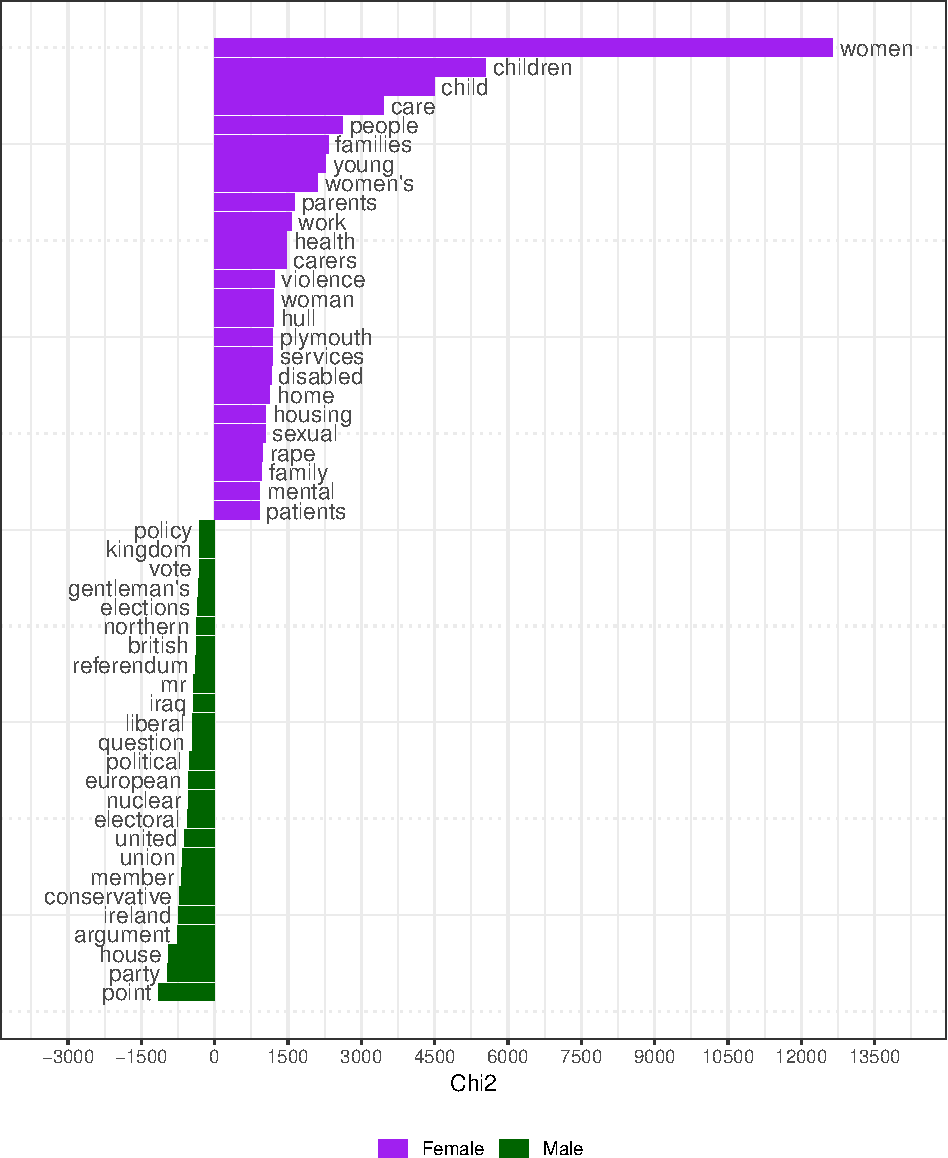
\includegraphics{methodology_files/figure-latex/gender-keyness-plot-1.pdf}
\caption{\label{fig:gender-keyness-plot}Keyness between Labour MPs, by
Gender}
\end{figure}

\hypertarget{shortlists-vs-non-shortlists-1}{%
\subsubsection{Shortlists vs
Non-Shortlists}\label{shortlists-vs-non-shortlists-1}}

Keyness differences by selection process (Figure \ref{fig:sl-keyness})
are not as obviously stereotypical. Nonetheless, the most common words
amongst AWS MPs included ``carers'', ``disabled'', ``bedroom'' and
``sen'' (Special Educational Needs). Also of note is AWS MPs making more
references to their ``constituency'' and its ``constituents'',
suggesting that AWS MPs may draw more heavily on the fact they were
elected by their constituents as a source political legitimacy, or are
more likely to illustrate a point with an example from their
constitutency, compared to non-AWS MPs.

\begin{figure}
\centering
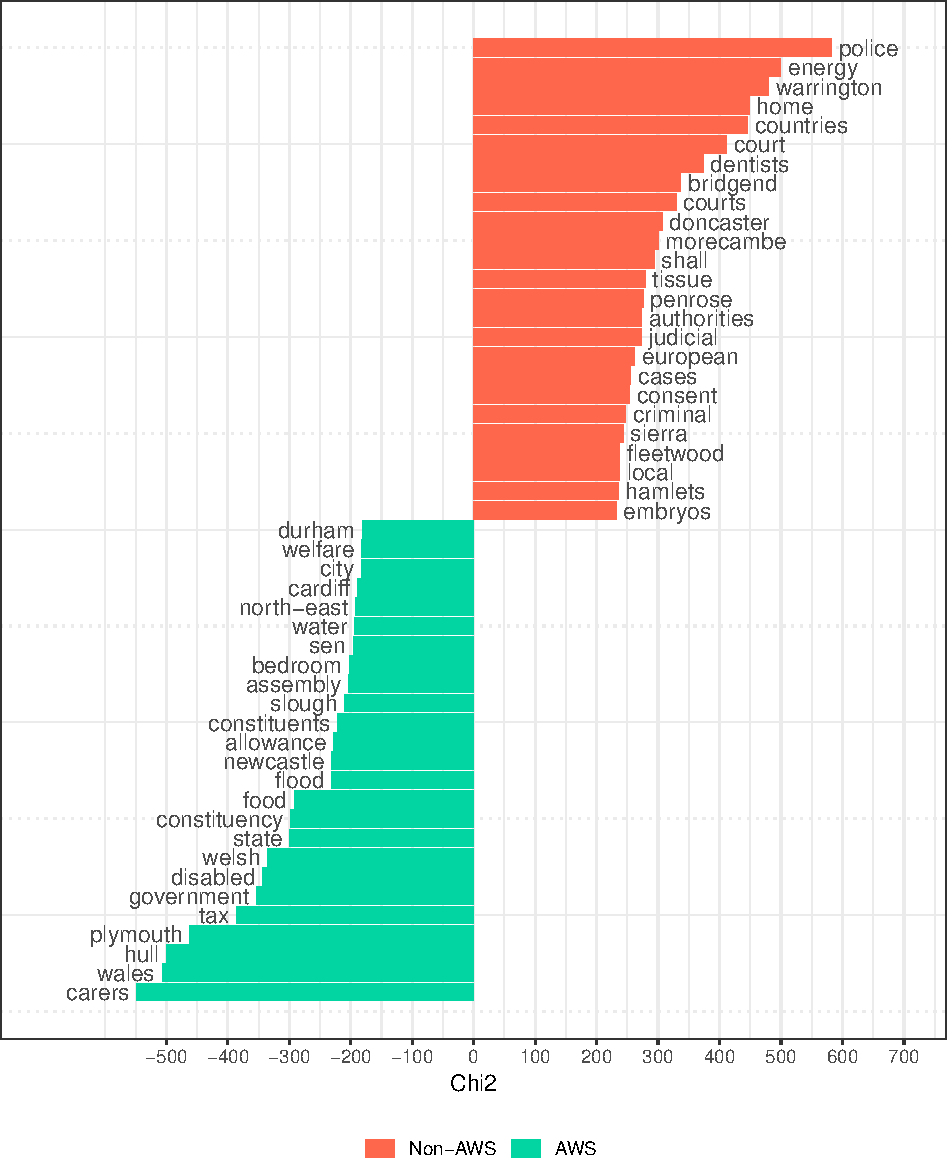
\includegraphics{methodology_files/figure-latex/sl-keyness-1.pdf}
\caption{\label{fig:sl-keyness}Keyness between Female Labour MPs, by
Selection Process}
\end{figure}

\hypertarget{labour-vs-conservative}{%
\subsubsection{Labour vs Conservative}\label{labour-vs-conservative}}

The keyness differences (Figure \ref{fig:lab-con-keyness}) between
Labour and Conservative MPs are much greater than gender or AWS
differences within Labour. The very high use of ``Lady'' by Conservative
MPs is reflective of the greater proportion of female MPs in other
parties, as it is often used to refer to comments by other members of
the house. It may also represent a greater use of traditional house
decorum by Conservative MPs.

\begin{figure}
\centering
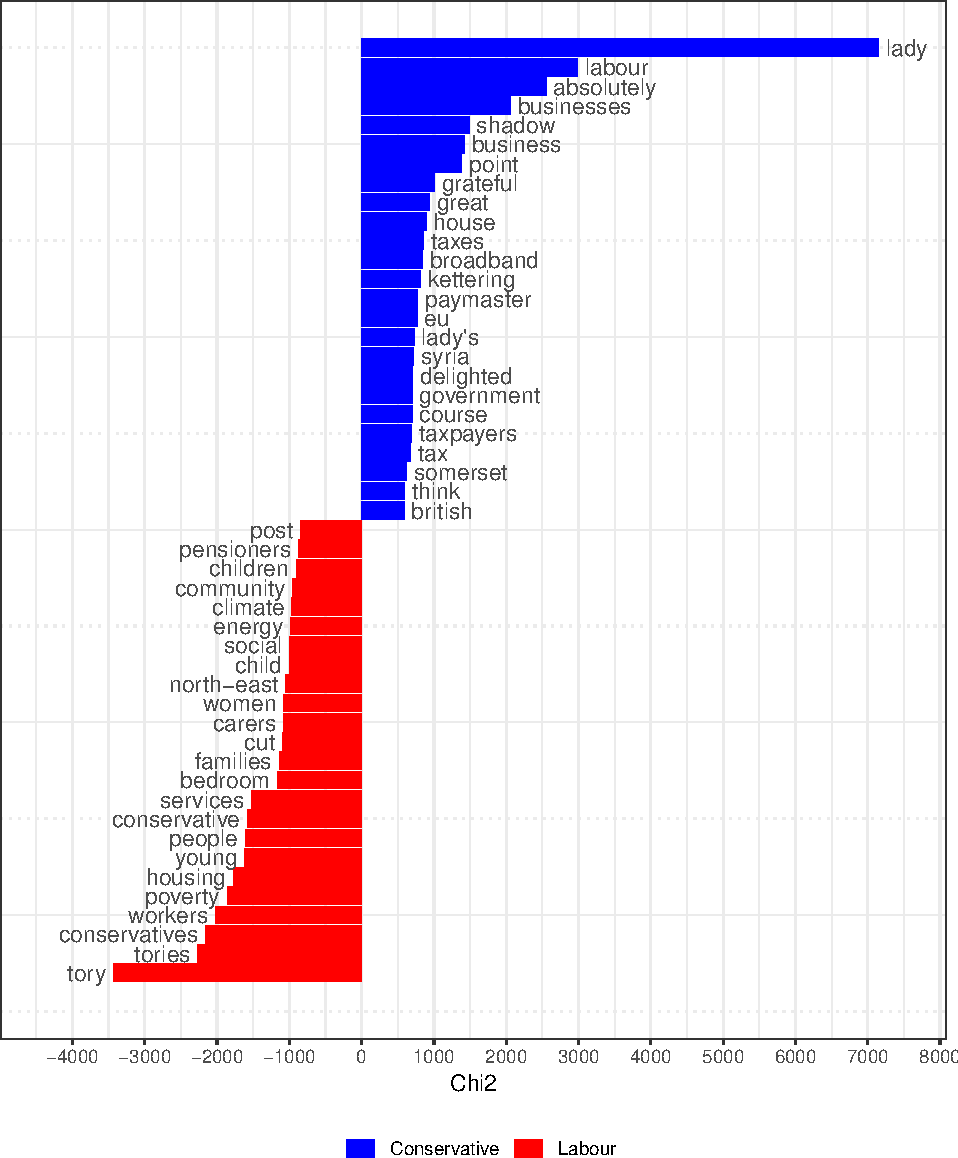
\includegraphics{methodology_files/figure-latex/lab-con-keyness-1.pdf}
\caption{\label{fig:lab-con-keyness}Keyness between Labour and Conservative
MPs}
\end{figure}

\hypertarget{bigrams}{%
\subsection{Bigrams}\label{bigrams}}

We created bigrams of all first person plural and singular pronouns for
female Labour MPs (Figure \ref{fig:bigrams-sl-keyness}). As above, AWS
MPs are far more likely to make references to their constituency or
their constituents, and the use of bigrams confirms these references are
to their specific constituency/constituents, rather than those of other
MPs, or constituencies in general.

\begin{figure}
\centering
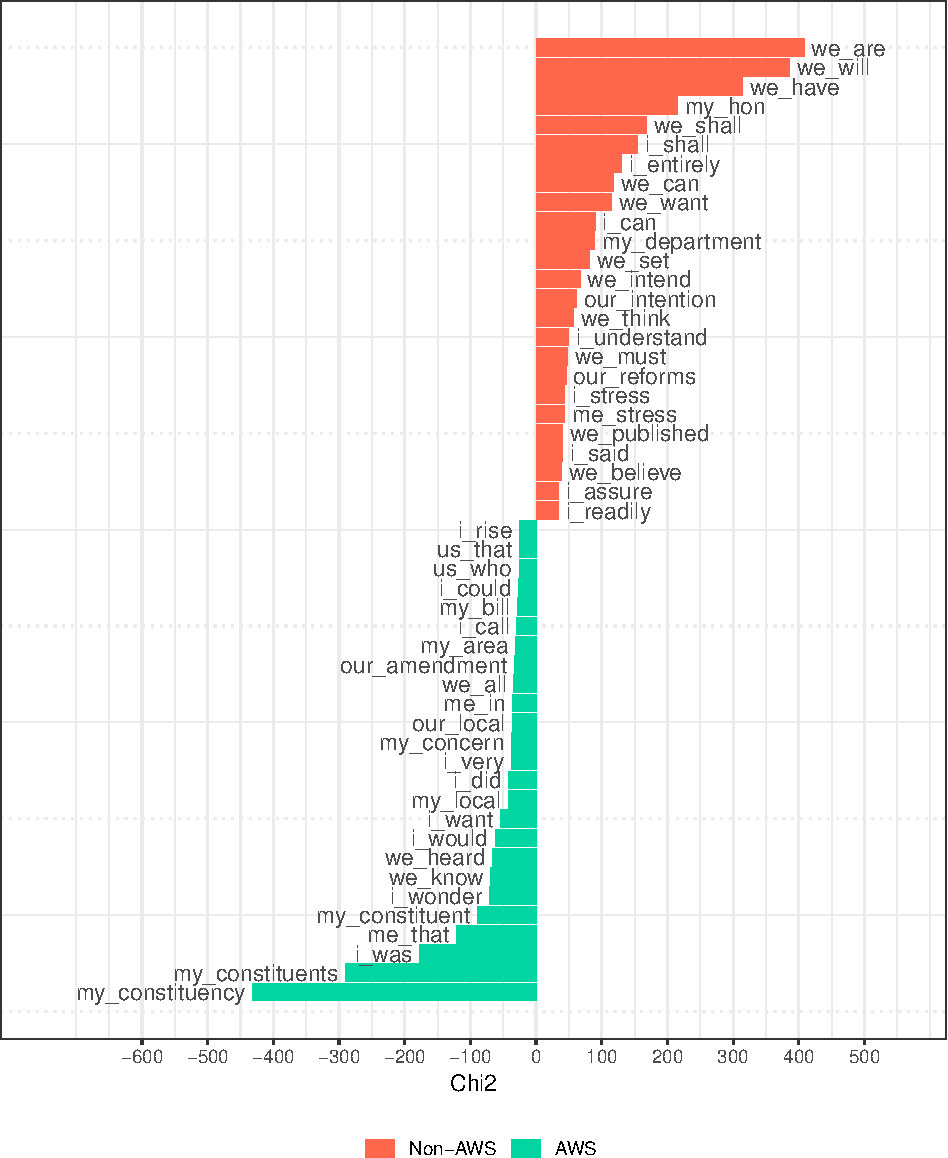
\includegraphics{methodology_files/figure-latex/bigrams-sl-keyness-1.pdf}
\caption{\label{fig:bigrams-sl-keyness}Bigram Keyness in Female Labour MPs
by Selection Process}
\end{figure}

\hypertarget{naive-bayes-classification}{%
\subsection{Naive Bayes
classification}\label{naive-bayes-classification}}

We trained a Naive Bayes classifier with document-frequency priors and a
multinomial distribution to predict the gender of speakers when given
speeches by all Labour MPs in our dataset, and the selection process
when only given female Labour MPs. The accuracy of both models were
roughly equivalent, 70.67\% accuracy when predicting gender and 71.22\%
when predicting shortlists. By contrast, the classifier could
distinguish between Labour and Conservative speeches with 74.23\%
accuracy.

\hypertarget{topic-models}{%
\subsection{Topic Models}\label{topic-models}}

Using topic models to classify text is widely used in social sciences
(Grimmer \& Stewart, \protect\hyperlink{ref-grimmer2013}{2013}), as,
when combined with the large volume of plain text data available, it
allows for a rapid and consistent method of analysis . Topic modelling
and other statistic methods of textual analysis are not a substitute for
reading the texts themselves, but can augment other analysis or -- as in
this case -- analyse and classify larger amounts of text than would be
feasible using human coders (Grimmer \& Stewart,
\protect\hyperlink{ref-grimmer2013}{2013}). Topic models classify a
series of documents (in this case individual speeches) into one of a
given number of topics, identifying terms that are common in some
documents but rare in others. When developing topic models, there is a
trade-off between high precision in the classification of each document
with broader topics when using smaller numbers of topics, or lower
precision in individual speech classification with more finely-grained
topics when using larger numbers of topics. Grimmer \& Stewart
(\protect\hyperlink{ref-grimmer2013}{2013}) also highlight the
importance of validating unsurpervised topic models when applied to new
sets of texts, which we have done
\protect\hyperlink{Manualux5cux2520Validation}{below}.

The R package \texttt{stm} (Roberts, Stewart, \& Tingley,
\protect\hyperlink{ref-roberts2018}{2018}) implements a structured topic
model (STM) (Arora et al., \protect\hyperlink{ref-arora2013}{2013};
Roberts, Stewart, \& Airoldi,
\protect\hyperlink{ref-roberts2016}{2016}). An STM incorporates
covariates into the topic classification algorithm, creating
possibilities for hypothesis testing. This differs from traditional
topic modelling methods using latent variables to identify topics
(e.g.~with latent Dirichlet allocation Blei, Ng, \& Jordan,
\protect\hyperlink{ref-blei2003}{2003}), and then comparing proportions
of each topic to one or more external variables. STM allows us to
incorporate the variables we are interested in to the topic model itself
using a generalised linear model; i.e.~the proportion of speechs
classified as belonging to each topic can vary as a function of the AWS
and gender variables.

We incorporated the AWS status of speakers and their gender as
prevalence covariates into our topic model.

We created six topic models with different numbers of topics (\emph{K}).
We created models with 30, 45, 60, 80 and 100 topics, and used a topic
selection algorithm developed by Lee \& Mimno
(\protect\hyperlink{ref-lee2014c}{2014}), implemented in the
\texttt{stm} package (Roberts et al.,
\protect\hyperlink{ref-roberts2018}{2018}), which resulted in \emph{K} =
66. Figure \ref{fig:topic-model-selection-plot} shows, clockwise from
the top-left, the exclusivity score, held out likelihood with 50\% of
documents held out, the multinomial dispersion of the STM residuals
(Taddy, \protect\hyperlink{ref-taddy2012}{2012}), semantic coherence
(Mimno, Wallach, Talley, Leenders, \& McCallum,
\protect\hyperlink{ref-mimno2011}{2011}), and the lower bound of each
topic model.

\begin{figure}
\centering
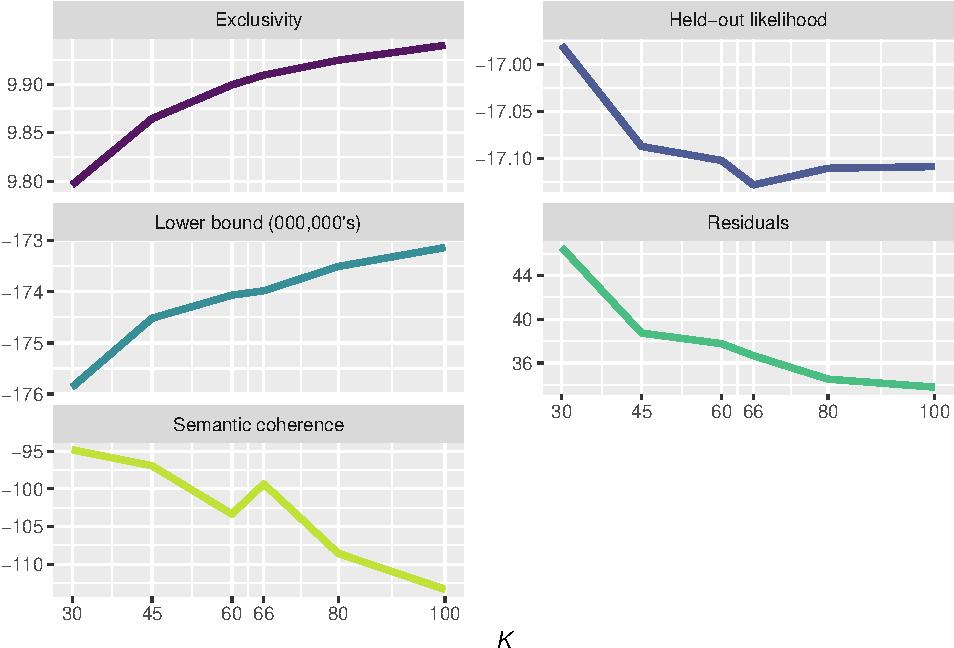
\includegraphics{methodology_files/figure-latex/topic-model-selection-plot-1.pdf}
\caption{\label{fig:topic-model-selection-plot}Topic Model Selection}
\end{figure}

As seen in Figure \ref{fig:topic-model-selection-plot}, the \emph{K} =
66 result appears to produce the best result, a topic model with 66
topics, across 251,072 speeches with a dictionary of 241,625 words. All
models were created using the ``spectral'' method developed by Arora et
al. (\protect\hyperlink{ref-arora2013}{2013}), implemented in the
\texttt{stm} package by Roberts et al.
(\protect\hyperlink{ref-roberts2018}{2018}).

Figure \ref{fig:stm-network-graph} is a Fruchterman-Reingold
force-directed diagram (Fruchterman \& Reingold,
\protect\hyperlink{ref-fruchterman1991}{1991}) of correlations between
different topics. Larger vertices indicate more common topics (amongst
both male and female Labour MPs), and the colour scale indicates the
proportion of speeches classed in that topic made by AWS and non-AWS
female Labour MPs, respectively. Edges indicate positive correlations
between the two linked topics.

\begin{figure}
\centering
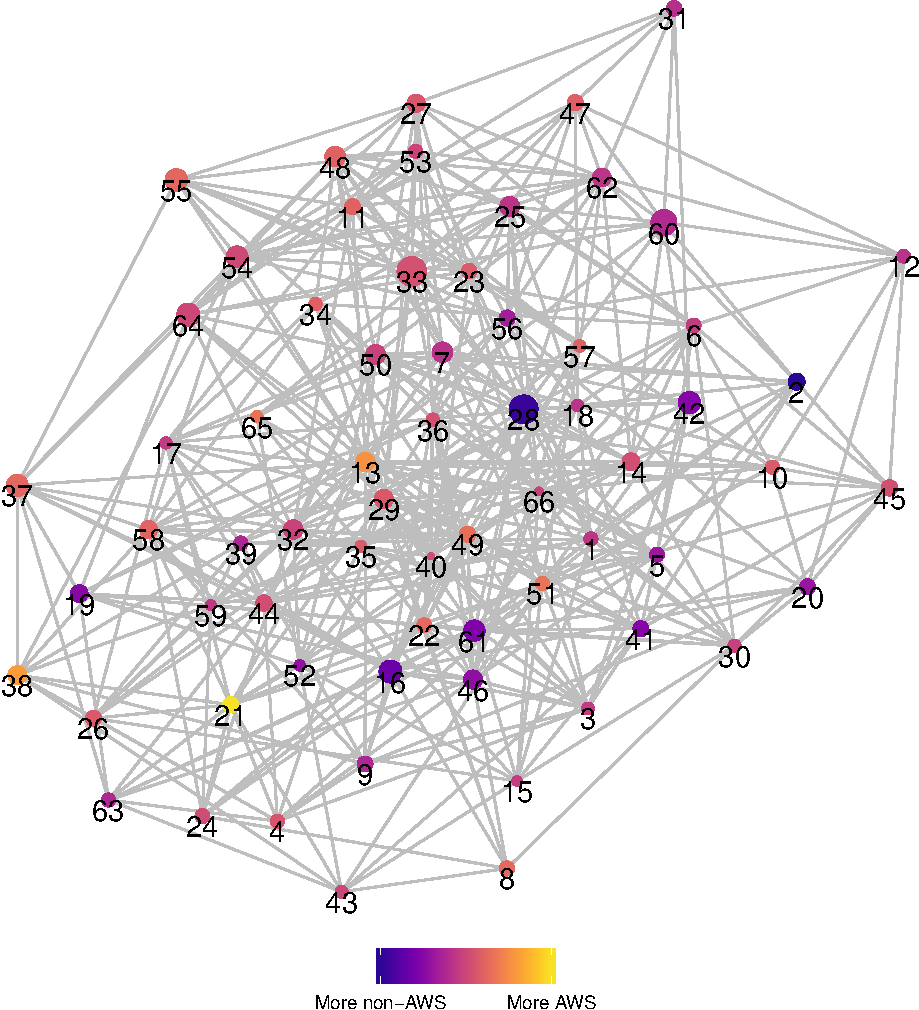
\includegraphics{methodology_files/figure-latex/stm-network-graph-1.pdf}
\caption{\label{fig:stm-network-graph}Fruchterman-Reingold plot of Topic
Network}
\end{figure}

The \texttt{stm} package includes the \texttt{estimateEffect} function,
which creates a regression model (Table \ref{tab:estimate-table-k0})
using individual documents (speeches) as observations, with the
proportion of a each document fitting each topic as the dependent
variable and model covariates (AWS status and gender) as independent
variables. The intercept in this model is all speeches by male Labour
MPs.

\begin{longtabu} to \linewidth {>{\raggedright}X>{\raggedleft}X>{\raggedleft}X>{\raggedleft}X>{\raggedleft}X>{\raggedright}X}
\caption{\label{tab:estimate-table-k0}Topic Estimates}\\
\toprule
 &  & Estimate & Standard Error & t value & Pr(>|t|)\\
\midrule
\endfirsthead
\caption[]{\label{tab:estimate-table-k0}Topic Estimates \textit{(continued)}}\\
\toprule
 &  & Estimate & Standard Error & t value & Pr(>|t|)\\
\midrule
\endhead
\
\endfoot
\bottomrule
\endlastfoot
 & Intercept & 0.0120888 & 0.0001178 & 102.6207609 & < 0.001 ***\\
\cmidrule{2-6}
 & Non-AWS & -0.0003789 & 0.0003148 & -1.2036179 & 0.23\\
\cmidrule{2-6}
\multirow{-3}{*}{\raggedright\arraybackslash (1) Employment \& unions} & AWS & -0.0013465 & 0.0002461 & -5.4715603 & < 0.001 ***\\
\cmidrule{1-6}
 & Intercept & 0.0167059 & 0.0001793 & 93.1509772 & < 0.001 ***\\
\cmidrule{2-6}
 & Non-AWS & 0.0069636 & 0.0005470 & 12.7297775 & < 0.001 ***\\
\cmidrule{2-6}
\multirow{-3}{*}{\raggedright\arraybackslash (2) Legal system} & AWS & -0.0033126 & 0.0003299 & -10.0398744 & < 0.001 ***\\
\cmidrule{1-6}
 & Intercept & 0.0116653 & 0.0001534 & 76.0329657 & < 0.001 ***\\
\cmidrule{2-6}
 & Non-AWS & -0.0014865 & 0.0004064 & -3.6575949 & < 0.001 ***\\
\cmidrule{2-6}
\multirow{-3}{*}{\raggedright\arraybackslash (3) Roads} & AWS & -0.0019506 & 0.0002972 & -6.5626439 & < 0.001 ***\\
\cmidrule{1-6}
 & Intercept & 0.0112840 & 0.0001700 & 66.3851110 & < 0.001 ***\\
\cmidrule{2-6}
 & Non-AWS & 0.0044556 & 0.0004910 & 9.0743223 & < 0.001 ***\\
\cmidrule{2-6}
\multirow{-3}{*}{\raggedright\arraybackslash (4) Housing} & AWS & 0.0060384 & 0.0003726 & 16.2079091 & < 0.001 ***\\
\cmidrule{1-6}
 & Intercept & 0.0140706 & 0.0001766 & 79.6599038 & < 0.001 ***\\
\cmidrule{2-6}
 & Non-AWS & 0.0032594 & 0.0005306 & 6.1425132 & < 0.001 ***\\
\cmidrule{2-6}
\multirow{-3}{*}{\raggedright\arraybackslash (5) Police, firefighters \& prison} & AWS & -0.0003211 & 0.0003580 & -0.8968734 & 0.37\\
\cmidrule{1-6}
 & Intercept & 0.0089512 & 0.0000479 & 186.9687383 & < 0.001 ***\\
\cmidrule{2-6}
 & Non-AWS & 0.0000927 & 0.0001254 & 0.7393203 & 0.46\\
\cmidrule{2-6}
\multirow{-3}{*}{\raggedright\arraybackslash (6) Northern Ireland} & AWS & -0.0003742 & 0.0001135 & -3.2957187 & < 0.001 ***\\
\cmidrule{1-6}
 & Intercept & 0.0213286 & 0.0001401 & 152.2480371 & < 0.001 ***\\
\cmidrule{2-6}
 & Non-AWS & -0.0007067 & 0.0003755 & -1.8820056 & 0.060\\
\cmidrule{2-6}
\multirow{-3}{*}{\raggedright\arraybackslash (7) Committee} & AWS & -0.0019549 & 0.0002695 & -7.2543909 & < 0.001 ***\\
\cmidrule{1-6}
 & Intercept & 0.0147204 & 0.0001992 & 73.8942771 & < 0.001 ***\\
\cmidrule{2-6}
 & Non-AWS & -0.0009650 & 0.0005007 & -1.9273270 & 0.054\\
\cmidrule{2-6}
\multirow{-3}{*}{\raggedright\arraybackslash (8) Schools} & AWS & 0.0021256 & 0.0004195 & 5.0664763 & < 0.001 ***\\
\cmidrule{1-6}
 & Intercept & 0.0170560 & 0.0001989 & 85.7313081 & < 0.001 ***\\
\cmidrule{2-6}
 & Non-AWS & -0.0011700 & 0.0005276 & -2.2175468 & 0.027 *\\
\cmidrule{2-6}
\multirow{-3}{*}{\raggedright\arraybackslash (9) Energy \& climate change} & AWS & -0.0035130 & 0.0004327 & -8.1187179 & < 0.001 ***\\
\cmidrule{1-6}
 & Intercept & 0.0157885 & 0.0001961 & 80.4931880 & < 0.001 ***\\
\cmidrule{2-6}
 & Non-AWS & -0.0075479 & 0.0004673 & -16.1523984 & < 0.001 ***\\
\cmidrule{2-6}
\multirow{-3}{*}{\raggedright\arraybackslash (10) Defence} & AWS & -0.0054199 & 0.0003717 & -14.5803283 & < 0.001 ***\\
\cmidrule{1-6}
 & Intercept & 0.0118988 & 0.0000782 & 152.2137390 & < 0.001 ***\\
\cmidrule{2-6}
 & Non-AWS & -0.0036969 & 0.0001975 & -18.7170311 & < 0.001 ***\\
\cmidrule{2-6}
\multirow{-3}{*}{\raggedright\arraybackslash (11) Parliament} & AWS & -0.0010975 & 0.0001545 & -7.1029189 & < 0.001 ***\\
\cmidrule{1-6}
 & Intercept & 0.0126074 & 0.0001317 & 95.7202390 & < 0.001 ***\\
\cmidrule{2-6}
 & Non-AWS & -0.0042376 & 0.0003207 & -13.2148342 & < 0.001 ***\\
\cmidrule{2-6}
\multirow{-3}{*}{\raggedright\arraybackslash (12) International politics} & AWS & -0.0054751 & 0.0002571 & -21.2971219 & < 0.001 ***\\
\cmidrule{1-6}
 & Intercept & 0.0167425 & 0.0001100 & 152.1375443 & < 0.001 ***\\
\cmidrule{2-6}
 & Non-AWS & -0.0029751 & 0.0002869 & -10.3699452 & < 0.001 ***\\
\cmidrule{2-6}
\multirow{-3}{*}{\raggedright\arraybackslash (13) Ministers} & AWS & 0.0031476 & 0.0002360 & 13.3392646 & < 0.001 ***\\
\cmidrule{1-6}
 & Intercept & 0.0115301 & 0.0000456 & 252.8430854 & < 0.001 ***\\
\cmidrule{2-6}
 & Non-AWS & 0.0002514 & 0.0001393 & 1.8045725 & 0.071\\
\cmidrule{2-6}
\multirow{-3}{*}{\raggedright\arraybackslash (14) Policy impact} & AWS & 0.0013687 & 0.0001043 & 13.1181516 & < 0.001 ***\\
\cmidrule{1-6}
 & Intercept & 0.0048744 & 0.0001190 & 40.9513068 & < 0.001 ***\\
\cmidrule{2-6}
 & Non-AWS & 0.0123730 & 0.0003703 & 33.4134974 & < 0.001 ***\\
\cmidrule{2-6}
\multirow{-3}{*}{\raggedright\arraybackslash (15) Gender} & AWS & 0.0119844 & 0.0003383 & 35.4273254 & < 0.001 ***\\
\cmidrule{1-6}
 & Intercept & 0.0230391 & 0.0001296 & 177.7745625 & < 0.001 ***\\
\cmidrule{2-6}
 & Non-AWS & 0.0070479 & 0.0003631 & 19.4089078 & < 0.001 ***\\
\cmidrule{2-6}
\multirow{-3}{*}{\raggedright\arraybackslash (16) Regional development} & AWS & 0.0002662 & 0.0002556 & 1.0417083 & 0.30\\
\cmidrule{1-6}
 & Intercept & 0.0097590 & 0.0001216 & 80.2448598 & < 0.001 ***\\
\cmidrule{2-6}
 & Non-AWS & -0.0006791 & 0.0003558 & -1.9084009 & 0.056\\
\cmidrule{2-6}
\multirow{-3}{*}{\raggedright\arraybackslash (17) Communications} & AWS & -0.0012030 & 0.0002652 & -4.5359044 & < 0.001 ***\\
\cmidrule{1-6}
 & Intercept & 0.0087070 & 0.0000954 & 91.2701772 & < 0.001 ***\\
\cmidrule{2-6}
 & Non-AWS & 0.0007389 & 0.0002708 & 2.7288967 & 0.006 **\\
\cmidrule{2-6}
\multirow{-3}{*}{\raggedright\arraybackslash (18) Immigration} & AWS & -0.0004165 & 0.0001877 & -2.2188444 & 0.026 *\\
\cmidrule{1-6}
 & Intercept & 0.0161560 & 0.0002152 & 75.0578742 & < 0.001 ***\\
\cmidrule{2-6}
 & Non-AWS & 0.0112569 & 0.0006412 & 17.5569007 & < 0.001 ***\\
\cmidrule{2-6}
\multirow{-3}{*}{\raggedright\arraybackslash (19) Health system} & AWS & 0.0062978 & 0.0004711 & 13.3680540 & < 0.001 ***\\
\cmidrule{1-6}
 & Intercept & 0.0160721 & 0.0002007 & 80.0858640 & < 0.001 ***\\
\cmidrule{2-6}
 & Non-AWS & 0.0004169 & 0.0005295 & 0.7874512 & 0.43\\
\cmidrule{2-6}
\multirow{-3}{*}{\raggedright\arraybackslash (20) International development} & AWS & -0.0033585 & 0.0003930 & -8.5459568 & < 0.001 ***\\
\cmidrule{1-6}
 & Intercept & 0.0120356 & 0.0001420 & 84.7801002 & < 0.001 ***\\
\cmidrule{2-6}
 & Non-AWS & 0.0009219 & 0.0003825 & 2.4103441 & 0.016 *\\
\cmidrule{2-6}
\multirow{-3}{*}{\raggedright\arraybackslash (21) Benefits \& disability} & AWS & 0.0120237 & 0.0003162 & 38.0267946 & < 0.001 ***\\
\cmidrule{1-6}
 & Intercept & 0.0127186 & 0.0001621 & 78.4784337 & < 0.001 ***\\
\cmidrule{2-6}
 & Non-AWS & -0.0024710 & 0.0004093 & -6.0365993 & < 0.001 ***\\
\cmidrule{2-6}
\multirow{-3}{*}{\raggedright\arraybackslash (22) Sport \& culture} & AWS & 0.0007438 & 0.0003253 & 2.2865634 & 0.022 *\\
\cmidrule{1-6}
 & Intercept & 0.0137409 & 0.0001075 & 127.8576615 & < 0.001 ***\\
\cmidrule{2-6}
 & Non-AWS & -0.0060868 & 0.0002725 & -22.3355410 & < 0.001 ***\\
\cmidrule{2-6}
\multirow{-3}{*}{\raggedright\arraybackslash (23) History} & AWS & -0.0040067 & 0.0002053 & -19.5138660 & < 0.001 ***\\
\cmidrule{1-6}
 & Intercept & 0.0143147 & 0.0001663 & 86.1011887 & < 0.001 ***\\
\cmidrule{2-6}
 & Non-AWS & -0.0010212 & 0.0004363 & -2.3408242 & 0.019 *\\
\cmidrule{2-6}
\multirow{-3}{*}{\raggedright\arraybackslash (24) Higher education \& skills} & AWS & -0.0001187 & 0.0003390 & -0.3501880 & 0.73\\
\cmidrule{1-6}
 & Intercept & 0.0155251 & 0.0000455 & 341.5239093 & < 0.001 ***\\
\cmidrule{2-6}
 & Non-AWS & -0.0018965 & 0.0001198 & -15.8370625 & < 0.001 ***\\
\cmidrule{2-6}
\multirow{-3}{*}{\raggedright\arraybackslash (25) Concurring point} & AWS & -0.0030028 & 0.0000881 & -34.0822282 & < 0.001 ***\\
\cmidrule{1-6}
 & Intercept & 0.0146922 & 0.0001644 & 89.3585721 & < 0.001 ***\\
\cmidrule{2-6}
 & Non-AWS & 0.0007062 & 0.0004256 & 1.6591475 & 0.097\\
\cmidrule{2-6}
\multirow{-3}{*}{\raggedright\arraybackslash (26) Pensions} & AWS & 0.0026268 & 0.0003314 & 7.9260121 & < 0.001 ***\\
\cmidrule{1-6}
 & Intercept & 0.0177826 & 0.0001289 & 137.9560812 & < 0.001 ***\\
\cmidrule{2-6}
 & Non-AWS & -0.0065299 & 0.0003217 & -20.2995950 & < 0.001 ***\\
\cmidrule{2-6}
\multirow{-3}{*}{\raggedright\arraybackslash (27) Points of order} & AWS & -0.0048147 & 0.0002501 & -19.2542330 & < 0.001 ***\\
\cmidrule{1-6}
 & Intercept & 0.0344876 & 0.0000989 & 348.5758700 & < 0.001 ***\\
\cmidrule{2-6}
 & Non-AWS & 0.0070279 & 0.0002802 & 25.0789103 & < 0.001 ***\\
\cmidrule{2-6}
\multirow{-3}{*}{\raggedright\arraybackslash (28) Issues} & AWS & -0.0025848 & 0.0001992 & -12.9759967 & < 0.001 ***\\
\cmidrule{1-6}
 & Intercept & 0.0131823 & 0.0000487 & 270.4829494 & < 0.001 ***\\
\cmidrule{2-6}
 & Non-AWS & 0.0011043 & 0.0001413 & 7.8140933 & < 0.001 ***\\
\cmidrule{2-6}
\multirow{-3}{*}{\raggedright\arraybackslash (29) Constituencies} & AWS & 0.0029672 & 0.0001077 & 27.5623637 & < 0.001 ***\\
\cmidrule{1-6}
 & Intercept & 0.0085769 & 0.0000759 & 113.0238684 & < 0.001 ***\\
\cmidrule{2-6}
 & Non-AWS & 0.0019127 & 0.0002216 & 8.6305954 & < 0.001 ***\\
\cmidrule{2-6}
\multirow{-3}{*}{\raggedright\arraybackslash (30) Ethnic groups \& racism} & AWS & 0.0019284 & 0.0001713 & 11.2560787 & < 0.001 ***\\
\cmidrule{1-6}
 & Intercept & 0.0149888 & 0.0001574 & 95.2276588 & < 0.001 ***\\
\cmidrule{2-6}
 & Non-AWS & -0.0017672 & 0.0004317 & -4.0930192 & < 0.001 ***\\
\cmidrule{2-6}
\multirow{-3}{*}{\raggedright\arraybackslash (31) Amendments} & AWS & -0.0033169 & 0.0003271 & -10.1410478 & < 0.001 ***\\
\cmidrule{1-6}
 & Intercept & 0.0169545 & 0.0001051 & 161.3924505 & < 0.001 ***\\
\cmidrule{2-6}
 & Non-AWS & 0.0012142 & 0.0002876 & 4.2211628 & < 0.001 ***\\
\cmidrule{2-6}
\multirow{-3}{*}{\raggedright\arraybackslash (32) Reports} & AWS & 0.0013433 & 0.0002351 & 5.7149497 & < 0.001 ***\\
\cmidrule{1-6}
 & Intercept & 0.0377535 & 0.0001141 & 330.9959877 & < 0.001 ***\\
\cmidrule{2-6}
 & Non-AWS & -0.0022839 & 0.0002856 & -7.9959376 & < 0.001 ***\\
\cmidrule{2-6}
\multirow{-3}{*}{\raggedright\arraybackslash (33) People} & AWS & -0.0010469 & 0.0002403 & -4.3563656 & < 0.001 ***\\
\cmidrule{1-6}
 & Intercept & 0.0135426 & 0.0001626 & 83.3072241 & < 0.001 ***\\
\cmidrule{2-6}
 & Non-AWS & -0.0047668 & 0.0003660 & -13.0248683 & < 0.001 ***\\
\cmidrule{2-6}
\multirow{-3}{*}{\raggedright\arraybackslash (34) Wales \& Scotland} & AWS & -0.0023237 & 0.0003017 & -7.7013426 & < 0.001 ***\\
\cmidrule{1-6}
 & Intercept & 0.0108970 & 0.0001602 & 68.0157187 & < 0.001 ***\\
\cmidrule{2-6}
 & Non-AWS & -0.0008332 & 0.0004344 & -1.9179306 & 0.055\\
\cmidrule{2-6}
\multirow{-3}{*}{\raggedright\arraybackslash (35) Alcohol \& tobacco} & AWS & 0.0011896 & 0.0003157 & 3.7684825 & < 0.001 ***\\
\cmidrule{1-6}
 & Intercept & 0.0083687 & 0.0000669 & 125.1467071 & < 0.001 ***\\
\cmidrule{2-6}
 & Non-AWS & 0.0000215 & 0.0001852 & 0.1160818 & 0.91\\
\cmidrule{2-6}
\multirow{-3}{*}{\raggedright\arraybackslash (36) Place names} & AWS & 0.0011694 & 0.0001457 & 8.0260801 & < 0.001 ***\\
\cmidrule{1-6}
 & Intercept & 0.0246559 & 0.0001707 & 144.4057423 & < 0.001 ***\\
\cmidrule{2-6}
 & Non-AWS & -0.0023121 & 0.0004551 & -5.0808110 & < 0.001 ***\\
\cmidrule{2-6}
\multirow{-3}{*}{\raggedright\arraybackslash (37) Budget} & AWS & 0.0007186 & 0.0003700 & 1.9421831 & 0.052\\
\cmidrule{1-6}
 & Intercept & 0.0193463 & 0.0001839 & 105.2177025 & < 0.001 ***\\
\cmidrule{2-6}
 & Non-AWS & -0.0013507 & 0.0005222 & -2.5866393 & 0.010 **\\
\cmidrule{2-6}
\multirow{-3}{*}{\raggedright\arraybackslash (38) Tax} & AWS & 0.0054452 & 0.0003801 & 14.3241563 & < 0.001 ***\\
\cmidrule{1-6}
 & Intercept & 0.0123822 & 0.0001231 & 100.5622646 & < 0.001 ***\\
\cmidrule{2-6}
 & Non-AWS & 0.0005476 & 0.0003530 & 1.5512923 & 0.12\\
\cmidrule{2-6}
\multirow{-3}{*}{\raggedright\arraybackslash (39) Private companies} & AWS & -0.0017986 & 0.0002410 & -7.4637103 & < 0.001 ***\\
\cmidrule{1-6}
 & Intercept & 0.0094593 & 0.0001554 & 60.8703332 & < 0.001 ***\\
\cmidrule{2-6}
 & Non-AWS & -0.0030966 & 0.0003590 & -8.6256246 & < 0.001 ***\\
\cmidrule{2-6}
\multirow{-3}{*}{\raggedright\arraybackslash (40) Environment \& fishing} & AWS & -0.0021431 & 0.0002972 & -7.2104552 & < 0.001 ***\\
\cmidrule{1-6}
 & Intercept & 0.0141414 & 0.0001678 & 84.2838152 & < 0.001 ***\\
\cmidrule{2-6}
 & Non-AWS & 0.0086017 & 0.0005357 & 16.0583471 & < 0.001 ***\\
\cmidrule{2-6}
\multirow{-3}{*}{\raggedright\arraybackslash (41) Crime} & AWS & 0.0034713 & 0.0003588 & 9.6742449 & < 0.001 ***\\
\cmidrule{1-6}
 & Intercept & 0.0244505 & 0.0001479 & 165.3707381 & < 0.001 ***\\
\cmidrule{2-6}
 & Non-AWS & 0.0021315 & 0.0004154 & 5.1316135 & < 0.001 ***\\
\cmidrule{2-6}
\multirow{-3}{*}{\raggedright\arraybackslash (42) Bills} & AWS & -0.0029731 & 0.0002794 & -10.6403551 & < 0.001 ***\\
\cmidrule{1-6}
 & Intercept & 0.0076732 & 0.0001334 & 57.5213940 & < 0.001 ***\\
\cmidrule{2-6}
 & Non-AWS & 0.0092120 & 0.0004022 & 22.9048156 & < 0.001 ***\\
\cmidrule{2-6}
\multirow{-3}{*}{\raggedright\arraybackslash (43) Children} & AWS & 0.0095672 & 0.0002849 & 33.5775063 & < 0.001 ***\\
\cmidrule{1-6}
 & Intercept & 0.0123341 & 0.0000950 & 129.8832950 & < 0.001 ***\\
\cmidrule{2-6}
 & Non-AWS & -0.0007809 & 0.0002313 & -3.3755091 & < 0.001 ***\\
\cmidrule{2-6}
\multirow{-3}{*}{\raggedright\arraybackslash (44) Utilities \& PFI} & AWS & 0.0002427 & 0.0001882 & 1.2893503 & 0.20\\
\cmidrule{1-6}
 & Intercept & 0.0174911 & 0.0002032 & 86.0965148 & < 0.001 ***\\
\cmidrule{2-6}
 & Non-AWS & -0.0028426 & 0.0005205 & -5.4610156 & < 0.001 ***\\
\cmidrule{2-6}
\multirow{-3}{*}{\raggedright\arraybackslash (45) Middle East} & AWS & -0.0017124 & 0.0004241 & -4.0379736 & < 0.001 ***\\
\cmidrule{1-6}
 & Intercept & 0.0179690 & 0.0001440 & 124.7990299 & < 0.001 ***\\
\cmidrule{2-6}
 & Non-AWS & 0.0044436 & 0.0004047 & 10.9809236 & < 0.001 ***\\
\cmidrule{2-6}
\multirow{-3}{*}{\raggedright\arraybackslash (46) Local authorities} & AWS & 0.0001255 & 0.0003158 & 0.3973772 & 0.69\\
\cmidrule{1-6}
 & Intercept & 0.0181760 & 0.0001744 & 104.2304478 & < 0.001 ***\\
\cmidrule{2-6}
 & Non-AWS & -0.0091719 & 0.0004160 & -22.0467462 & < 0.001 ***\\
\cmidrule{2-6}
\multirow{-3}{*}{\raggedright\arraybackslash (47) Elections} & AWS & -0.0068107 & 0.0003435 & -19.8249723 & < 0.001 ***\\
\cmidrule{1-6}
 & Intercept & 0.0180051 & 0.0000740 & 243.4560321 & < 0.001 ***\\
\cmidrule{2-6}
 & Non-AWS & -0.0034963 & 0.0001993 & -17.5442276 & < 0.001 ***\\
\cmidrule{2-6}
\multirow{-3}{*}{\raggedright\arraybackslash (48) Debate} & AWS & -0.0009781 & 0.0001463 & -6.6838588 & < 0.001 ***\\
\cmidrule{1-6}
 & Intercept & 0.0164409 & 0.0001990 & 82.6102476 & < 0.001 ***\\
\cmidrule{2-6}
 & Non-AWS & -0.0027435 & 0.0005152 & -5.3246978 & < 0.001 ***\\
\cmidrule{2-6}
\multirow{-3}{*}{\raggedright\arraybackslash (49) Transport} & AWS & 0.0008858 & 0.0003919 & 2.2601217 & 0.024 *\\
\cmidrule{1-6}
 & Intercept & 0.0161734 & 0.0000754 & 214.4489860 & < 0.001 ***\\
\cmidrule{2-6}
 & Non-AWS & 0.0001322 & 0.0001922 & 0.6881049 & 0.49\\
\cmidrule{2-6}
\multirow{-3}{*}{\raggedright\arraybackslash (50) Questions} & AWS & 0.0002167 & 0.0001602 & 1.3530847 & 0.18\\
\cmidrule{1-6}
 & Intercept & 0.0101064 & 0.0001123 & 90.0068284 & < 0.001 ***\\
\cmidrule{2-6}
 & Non-AWS & 0.0019112 & 0.0003357 & 5.6937074 & < 0.001 ***\\
\cmidrule{2-6}
\multirow{-3}{*}{\raggedright\arraybackslash (51) Families} & AWS & 0.0058679 & 0.0002503 & 23.4470168 & < 0.001 ***\\
\cmidrule{1-6}
 & Intercept & 0.0088047 & 0.0001527 & 57.6752383 & < 0.001 ***\\
\cmidrule{2-6}
 & Non-AWS & 0.0076317 & 0.0004412 & 17.2968701 & < 0.001 ***\\
\cmidrule{2-6}
\multirow{-3}{*}{\raggedright\arraybackslash (52) Health research} & AWS & 0.0036096 & 0.0003276 & 11.0195896 & < 0.001 ***\\
\cmidrule{1-6}
 & Intercept & 0.0075507 & 0.0000226 & 334.4435527 & < 0.001 ***\\
\cmidrule{2-6}
 & Non-AWS & -0.0011339 & 0.0000539 & -21.0226709 & < 0.001 ***\\
\cmidrule{2-6}
\multirow{-3}{*}{\raggedright\arraybackslash (53) Dispatch box} & AWS & -0.0009564 & 0.0000454 & -21.0477435 & < 0.001 ***\\
\cmidrule{1-6}
 & Intercept & 0.0248192 & 0.0001247 & 199.0509225 & < 0.001 ***\\
\cmidrule{2-6}
 & Non-AWS & -0.0066206 & 0.0003398 & -19.4818710 & < 0.001 ***\\
\cmidrule{2-6}
\multirow{-3}{*}{\raggedright\arraybackslash (54) Parties} & AWS & -0.0059979 & 0.0002615 & -22.9408627 & < 0.001 ***\\
\cmidrule{1-6}
 & Intercept & 0.0211142 & 0.0000693 & 304.7907001 & < 0.001 ***\\
\cmidrule{2-6}
 & Non-AWS & -0.0045072 & 0.0001847 & -24.3999682 & < 0.001 ***\\
\cmidrule{2-6}
\multirow{-3}{*}{\raggedright\arraybackslash (55) Statements} & AWS & -0.0014965 & 0.0001320 & -11.3348121 & < 0.001 ***\\
\cmidrule{1-6}
 & Intercept & 0.0163483 & 0.0001622 & 100.8162901 & < 0.001 ***\\
\cmidrule{2-6}
 & Non-AWS & -0.0024198 & 0.0004562 & -5.3044297 & < 0.001 ***\\
\cmidrule{2-6}
\multirow{-3}{*}{\raggedright\arraybackslash (56) European Union} & AWS & -0.0053884 & 0.0003326 & -16.2000849 & < 0.001 ***\\
\cmidrule{1-6}
 & Intercept & 0.0100671 & 0.0001093 & 92.1437166 & < 0.001 ***\\
\cmidrule{2-6}
 & Non-AWS & -0.0025131 & 0.0002671 & -9.4076381 & < 0.001 ***\\
\cmidrule{2-6}
\multirow{-3}{*}{\raggedright\arraybackslash (57) Locations} & AWS & 0.0000336 & 0.0002075 & 0.1618511 & 0.87\\
\cmidrule{1-6}
 & Intercept & 0.0175837 & 0.0001670 & 105.3211770 & < 0.001 ***\\
\cmidrule{2-6}
 & Non-AWS & -0.0016196 & 0.0004317 & -3.7511794 & < 0.001 ***\\
\cmidrule{2-6}
\multirow{-3}{*}{\raggedright\arraybackslash (58) Jobs \& manufacturing} & AWS & 0.0012056 & 0.0003445 & 3.4992705 & < 0.001 ***\\
\cmidrule{1-6}
 & Intercept & 0.0070669 & 0.0000724 & 97.5560125 & < 0.001 ***\\
\cmidrule{2-6}
 & Non-AWS & 0.0005501 & 0.0001993 & 2.7606461 & 0.006 **\\
\cmidrule{2-6}
\multirow{-3}{*}{\raggedright\arraybackslash (59) Small business} & AWS & -0.0003673 & 0.0001454 & -2.5262114 & 0.012 *\\
\cmidrule{1-6}
 & Intercept & 0.0328532 & 0.0001147 & 286.3644270 & < 0.001 ***\\
\cmidrule{2-6}
 & Non-AWS & -0.0089896 & 0.0003028 & -29.6843140 & < 0.001 ***\\
\cmidrule{2-6}
\multirow{-3}{*}{\raggedright\arraybackslash (60) Agreement \& disagreement} & AWS & -0.0109445 & 0.0002035 & -53.7940555 & < 0.001 ***\\
\cmidrule{1-6}
 & Intercept & 0.0187127 & 0.0001243 & 150.5063327 & < 0.001 ***\\
\cmidrule{2-6}
 & Non-AWS & 0.0111185 & 0.0003722 & 29.8746792 & < 0.001 ***\\
\cmidrule{2-6}
\multirow{-3}{*}{\raggedright\arraybackslash (61) Voluntary sector} & AWS & 0.0056586 & 0.0002496 & 22.6728341 & < 0.001 ***\\
\cmidrule{1-6}
 & Intercept & 0.0152725 & 0.0000669 & 228.1931718 & < 0.001 ***\\
\cmidrule{2-6}
 & Non-AWS & -0.0029228 & 0.0001709 & -17.1025255 & < 0.001 ***\\
\cmidrule{2-6}
\multirow{-3}{*}{\raggedright\arraybackslash (62) Comments} & AWS & -0.0040217 & 0.0001204 & -33.3916425 & < 0.001 ***\\
\cmidrule{1-6}
 & Intercept & 0.0090473 & 0.0001163 & 77.8049643 & < 0.001 ***\\
\cmidrule{2-6}
 & Non-AWS & 0.0094874 & 0.0003827 & 24.7908780 & < 0.001 ***\\
\cmidrule{2-6}
\multirow{-3}{*}{\raggedright\arraybackslash (63) Social care} & AWS & 0.0073846 & 0.0002802 & 26.3574994 & < 0.001 ***\\
\cmidrule{1-6}
 & Intercept & 0.0213818 & 0.0000679 & 314.7746216 & < 0.001 ***\\
\cmidrule{2-6}
 & Non-AWS & -0.0020761 & 0.0001751 & -11.8564587 & < 0.001 ***\\
\cmidrule{2-6}
\multirow{-3}{*}{\raggedright\arraybackslash (64) Time} & AWS & -0.0016514 & 0.0001432 & -11.5355536 & < 0.001 ***\\
\cmidrule{1-6}
 & Intercept & 0.0121387 & 0.0001644 & 73.8313247 & < 0.001 ***\\
\cmidrule{2-6}
 & Non-AWS & -0.0057090 & 0.0004043 & -14.1203754 & < 0.001 ***\\
\cmidrule{2-6}
\multirow{-3}{*}{\raggedright\arraybackslash (65) Media \& animals} & AWS & -0.0017755 & 0.0003183 & -5.5781252 & < 0.001 ***\\
\cmidrule{1-6}
 & Intercept & 0.0038249 & 0.0000114 & 334.6396884 & < 0.001 ***\\
\cmidrule{2-6}
 & Non-AWS & 0.0002529 & 0.0000292 & 8.6594542 & < 0.001 ***\\
\cmidrule{2-6}
\multirow{-3}{*}{\raggedright\arraybackslash (66) Other} & AWS & 0.0003060 & 0.0000249 & 12.2797016 & < 0.001 ***\\*
\end{longtabu}

Table \ref{tab:topic-summary-table} shows the number and percentage of
speeches assigned to each topic, based on its \(\theta\) value. The
results in this table differ slightly from those in Table
\ref{tab:estimate-table-k0}, as it uses a ``winner-take-all'' method to
assign an overall topic to each speech, rather than a prevalence of a
given topic across all speeches. One of the topics -- Topic 66 -- is
never the most likely topic in the matrix of number of documents by
number of topics -- labelled \(\theta\) by Roberts et al.
(\protect\hyperlink{ref-roberts2018}{2018}) -- and so while it is
included in the model, assignment of single topics to speeches uses the
highest \(\theta\) for each speech. Other topics are rarely used --
Topic 53, which we labelled ``Dispatch Box'', only has five topics
assigned to it, four from Male MPs and one from an AWS MP.

\begin{longtabu} to \linewidth {>{\raggedright\arraybackslash}p{5cm}>{\raggedleft}X>{\raggedleft}X>{\raggedleft}X>{\raggedleft}X>{\raggedleft}X>{\raggedleft}X}
\caption{\label{tab:topic-summary-table}Count and Distribution of Topics}\\
\toprule
Topic & AWS Speeches & Percent of AWS Speeches & Non-AWS Speeches & Percent of non-AWS Speeches & Male MP Speeches & Percent of Male MP Speeches\\
\midrule
\endfirsthead
\caption[]{\label{tab:topic-summary-table}Count and Distribution of Topics \textit{(continued)}}\\
\toprule
Topic & AWS Speeches & Percent of AWS Speeches & Non-AWS Speeches & Percent of non-AWS Speeches & Male MP Speeches & Percent of Male MP Speeches\\
\midrule
\endhead
\
\endfoot
\bottomrule
\endlastfoot
(1) Employment \& unions & 452 & 0.84\% & 260 & 0.93\% & 2,149 & 1.27\%\\
(2) Legal system & 865 & 1.61\% & 1,096 & 3.93\% & 3,884 & 2.29\%\\
(3) Roads & 558 & 1.04\% & 298 & 1.07\% & 2,142 & 1.26\%\\
(4) Housing & 1,383 & 2.57\% & 665 & 2.39\% & 2,416 & 1.43\%\\
(5) Police, firefighters \& prison & 1,046 & 1.94\% & 709 & 2.54\% & 3,353 & 1.98\%\\
\addlinespace
(6) Northern Ireland & 221 & 0.41\% & 66 & 0.24\% & 603 & 0.36\%\\
(7) Committee & 1,050 & 1.95\% & 492 & 1.77\% & 3,888 & 2.29\%\\
(8) Schools & 1,367 & 2.54\% & 522 & 1.87\% & 3,780 & 2.23\%\\
(9) Energy \& climate change & 1,105 & 2.05\% & 745 & 2.67\% & 4,630 & 2.73\%\\
(10) Defence & 794 & 1.48\% & 280 & 1.00\% & 3,999 & 2.36\%\\
\addlinespace
(11) Parliament & 375 & 0.70\% & 85 & 0.31\% & 1,079 & 0.64\%\\
(12) International politics & 289 & 0.54\% & 161 & 0.58\% & 2,021 & 1.19\%\\
(13) Ministers & 872 & 1.62\% & 242 & 0.87\% & 2,083 & 1.23\%\\
(14) Policy impact & 242 & 0.45\% & 68 & 0.24\% & 417 & 0.25\%\\
(15) Gender & 1,257 & 2.34\% & 701 & 2.52\% & 551 & 0.33\%\\
\addlinespace
(16) Regional development & 931 & 1.73\% & 710 & 2.55\% & 2,704 & 1.60\%\\
(17) Communications & 385 & 0.72\% & 287 & 1.03\% & 1,751 & 1.03\%\\
(18) Immigration & 425 & 0.79\% & 220 & 0.79\% & 1,218 & 0.72\%\\
(19) Health system & 2,149 & 4.00\% & 1,489 & 5.34\% & 4,682 & 2.76\%\\
(20) International development & 862 & 1.60\% & 687 & 2.47\% & 3,718 & 2.19\%\\
\addlinespace
(21) Benefits \& disability & 1,888 & 3.51\% & 317 & 1.14\% & 2,101 & 1.24\%\\
(22) Sport \& culture & 846 & 1.57\% & 317 & 1.14\% & 2,628 & 1.55\%\\
(23) History & 299 & 0.56\% & 140 & 0.50\% & 1,720 & 1.02\%\\
(24) Higher education \& skills & 974 & 1.81\% & 456 & 1.64\% & 3,501 & 2.07\%\\
(25) Concurring point & 33 & 0.06\% & 9 & 0.03\% & 139 & 0.08\%\\
\addlinespace
(26) Pensions & 1,231 & 2.29\% & 529 & 1.90\% & 2,982 & 1.76\%\\
(27) Points of order & 787 & 1.46\% & 230 & 0.83\% & 4,069 & 2.40\%\\
(28) Issues & 1,618 & 3.01\% & 1,720 & 6.17\% & 6,745 & 3.98\%\\
(29) Constituencies & 125 & 0.23\% & 30 & 0.11\% & 228 & 0.13\%\\
(30) Ethnic groups \& racism & 454 & 0.84\% & 203 & 0.73\% & 945 & 0.56\%\\
\addlinespace
(31) Amendments & 526 & 0.98\% & 317 & 1.14\% & 2,293 & 1.35\%\\
(32) Reports & 536 & 1.00\% & 322 & 1.16\% & 1,488 & 0.88\%\\
(33) People & 2,818 & 5.24\% & 1,048 & 3.76\% & 9,136 & 5.39\%\\
(34) Wales \& Scotland & 662 & 1.23\% & 224 & 0.80\% & 2,655 & 1.57\%\\
(35) Alcohol \& tobacco & 846 & 1.57\% & 336 & 1.21\% & 2,357 & 1.39\%\\
\addlinespace
(36) Place names & 163 & 0.30\% & 47 & 0.17\% & 447 & 0.26\%\\
(37) Budget & 1,616 & 3.00\% & 668 & 2.40\% & 5,567 & 3.29\%\\
(38) Tax & 2,149 & 4.00\% & 691 & 2.48\% & 4,562 & 2.69\%\\
(39) Private companies & 452 & 0.84\% & 362 & 1.30\% & 1,794 & 1.06\%\\
(40) Environment \& fishing & 435 & 0.81\% & 186 & 0.67\% & 1,689 & 1.00\%\\
\addlinespace
(41) Crime & 1,408 & 2.62\% & 926 & 3.32\% & 3,073 & 1.81\%\\
(42) Bills & 1,199 & 2.23\% & 931 & 3.34\% & 4,534 & 2.68\%\\
(43) Children & 1,176 & 2.19\% & 631 & 2.26\% & 1,298 & 0.77\%\\
(44) Utilities \& PFI & 433 & 0.81\% & 175 & 0.63\% & 1,416 & 0.84\%\\
(45) Middle East & 1,284 & 2.39\% & 588 & 2.11\% & 4,543 & 2.68\%\\
\addlinespace
(46) Local authorities & 1,050 & 1.95\% & 711 & 2.55\% & 3,686 & 2.18\%\\
(47) Elections & 759 & 1.41\% & 240 & 0.86\% & 4,308 & 2.54\%\\
(48) Debate & 422 & 0.78\% & 128 & 0.46\% & 1,364 & 0.81\%\\
(49) Transport & 1,517 & 2.82\% & 546 & 1.96\% & 4,172 & 2.46\%\\
(50) Questions & 390 & 0.73\% & 182 & 0.65\% & 1,115 & 0.66\%\\
\addlinespace
(51) Families & 786 & 1.46\% & 276 & 0.99\% & 1,169 & 0.69\%\\
(52) Health research & 743 & 1.38\% & 591 & 2.12\% & 1,467 & 0.87\%\\
(53) Dispatch box & 1 & 0.00\% & NA & NA\% & 4 & 0.00\%\\
(54) Parties & 879 & 1.63\% & 438 & 1.57\% & 5,053 & 2.98\%\\
(55) Statements & 180 & 0.33\% & 79 & 0.28\% & 856 & 0.51\%\\
\addlinespace
(56) European Union & 769 & 1.43\% & 554 & 1.99\% & 3,949 & 2.33\%\\
(57) Locations & 299 & 0.56\% & 126 & 0.45\% & 1,112 & 0.66\%\\
(58) Jobs \& manufacturing & 1,426 & 2.65\% & 586 & 2.10\% & 4,162 & 2.46\%\\
(59) Small business & 229 & 0.43\% & 183 & 0.66\% & 791 & 0.47\%\\
(60) Agreement \& disagreement & 523 & 0.97\% & 275 & 0.99\% & 4,962 & 2.93\%\\
\addlinespace
(61) Voluntary sector & 1,307 & 2.43\% & 853 & 3.06\% & 2,480 & 1.46\%\\
(62) Comments & 108 & 0.20\% & 95 & 0.34\% & 865 & 0.51\%\\
(63) Social care & 865 & 1.61\% & 521 & 1.87\% & 1,187 & 0.70\%\\
(64) Time & 208 & 0.39\% & 103 & 0.37\% & 930 & 0.55\%\\
(65) Media \& animals & 741 & 1.38\% & 190 & 0.68\% & 2,811 & 1.66\%\\*
\end{longtabu}

\hypertarget{topic-graphs}{%
\subsubsection{Topic Graphs}\label{topic-graphs}}

The estimate effects in these graphs were extracted using the
\texttt{tidystm} package by Mikael Poul Johannesson.\footnote{Available
  online at: \url{https://github.com/mikajoh/tidystm}} Figure
\ref{fig:tidystm-graphs} highlights nine topics with different expected
proportions between male, AWS and non-AWS Labour MPs, with the error
bars representing 95\% confidence intervals. See Figure
\ref{fig:topic-bar} for a graph of all 66 topics.

\begin{figure}
\centering
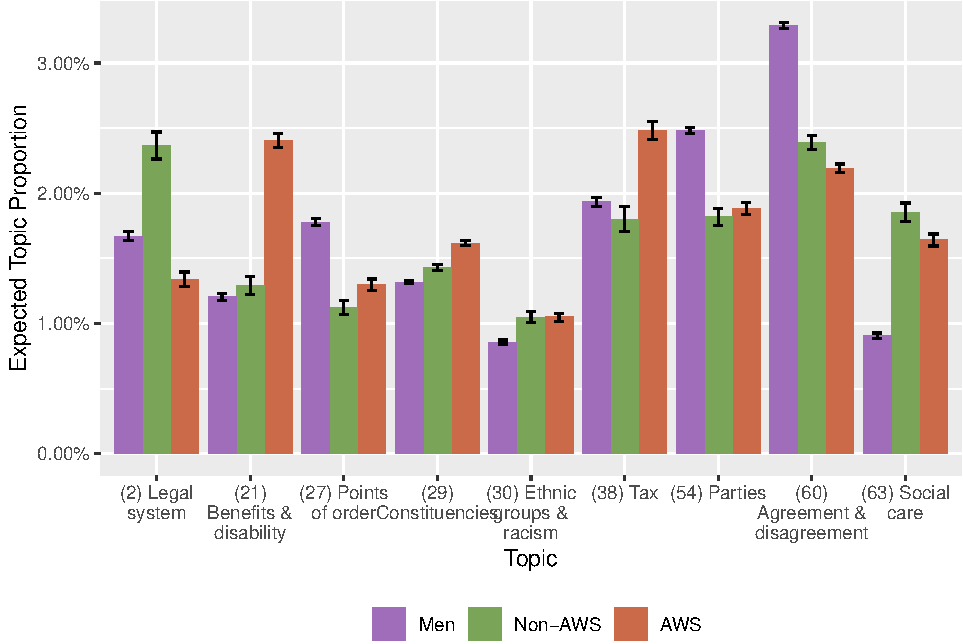
\includegraphics{methodology_files/figure-latex/tidystm-graphs-1.pdf}
\caption{\label{fig:tidystm-graphs}Selected Topic Proportions}
\end{figure}

\begin{figure}
\centering
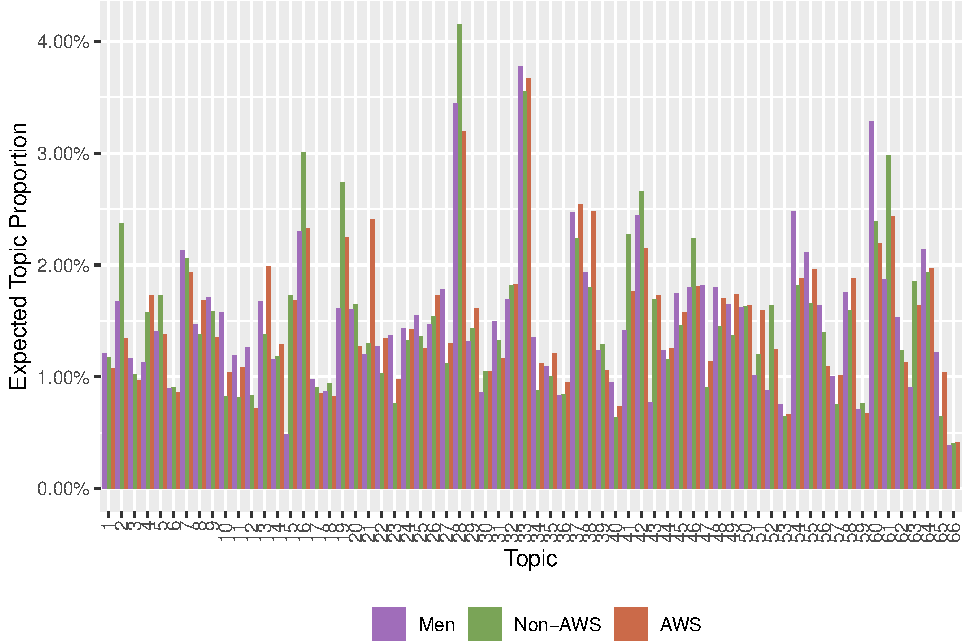
\includegraphics{methodology_files/figure-latex/topic-bar-1.pdf}
\caption{\label{fig:topic-bar}All Topic Proportions}
\end{figure}

\hypertarget{word-occurrences}{%
\subsubsection{Word Occurrences}\label{word-occurrences}}

The table below shows the twenty most common words in each topic, and
the twenty words with the highest FREX score, a measure that uses a
harmonic mean of word exclusivity and topic coherence (Airoldi \&
Bischof, \protect\hyperlink{ref-airoldi2016}{2016}). We have named each
topic based on the most common words and highest FREX score words in
each topic.

\begin{longtabu} to \linewidth {>{\raggedright}X>{\raggedright\arraybackslash}p{6cm}>{\raggedright\arraybackslash}p{6cm}}
\caption{\label{tab:topic-words-table-k0}Words in Topic}\\
\toprule
Topic & Top Twenty Words & Top Twenty FREX\\
\midrule
\endfirsthead
\caption[]{\label{tab:topic-words-table-k0}Words in Topic \textit{(continued)}}\\
\toprule
Topic & Top Twenty Words & Top Twenty FREX\\
\midrule
\endhead
\
\endfoot
\bottomrule
\endlastfoot
(1) Employment \& unions & rights, workers, law, human, civil, trade, union, protection, employers, act, employment, unions, safety, employees, work, service, staff, employer, legislation, protect & tupe, blacklisting, acas, rights, gangmasters, civil, dispute, protections, unions, dismissal, servants, human, disputes, workers, employer, num, certification, employees, tuc, employers\\
(2) Legal system & cases, court, legal, case, justice, law, courts, evidence, lord, appeal, system, criminal, judicial, investigation, judge, aid, prosecution, circumstances, trial, lawyers & judicial, attorney-general, court, prosecutor, judges, carlile, defendant, extradition, cps, judiciary, admissible, pre-charge, jury, solicitors, lawyers, solicitor, courts, lawyer, detention, judge\\
(3) Roads & road, planning, site, land, sites, car, vehicles, residents, roads, safety, use, driving, vehicle, park, development, traffic, drivers, area, cars, speed & bikes, cyclists, pedestrians, gypsy, off-road, cycling, encampments, parking, highways, masts, drivers, belt, roads, highway, road, gypsies, vehicles, site, vehicle, bike\\
(4) Housing & housing, homes, social, affordable, property, home, properties, london, accommodation, building, private, houses, tenants, rent, need, council, landlords, sector, buy, people & tenants, rent, landlords, rented, homelessness, rents, leaseholders, leasehold, tenancy, commonhold, hmos, housing, one-bedroom, homeless, properties, right-to-buy, affordable, sleepers, fulham, landlord\\
(5) Police, firefighters \& prison & police, officers, crime, policing, service, fire, prison, home, force, chief, community, officer, staff, forces, neighbourhood, probation, prisons, safety, prisoners, resources & policing, firefighters, constables, pcsos, probation, csos, prisons, fire, constable, hmic, constabulary, officers, police, prison, prisoners, reoffending, neighbourhood, metropolitan, fires, ipcc\\
\addlinespace
(6) Northern Ireland & make, sure, progress, northern, decisions, ireland, difference, towards, future, process, contribution, statement, responsibilities, easier, responsibility, must, departmental, belfast, friday, choices & sinn, fein, make, sure, belfast, northern, progress, ulster, difference, ireland, ruc, decisions, patten, dissident, departmental, taoiseach, antrim, imc, chastelain, dpps\\
(7) Committee & committee, report, review, commission, independent, government, select, process, evidence, inquiry, scrutiny, recommendations, role, board, set, work, reports, public, published, parliament & committee's, select, inquiry, scrutiny, recommendations, committee, committees, independent, recommendation, panel, pre-legislative, report, chairman, review, reviews, scrutinise, inquiries, conclusions, publication, findings\\
(8) Schools & schools, school, education, teachers, pupils, primary, children, standards, educational, special, secondary, parents, free, teacher, teaching, head, academies, academy, curriculum, good & schools, teachers, pupils, academies, pupil, grammar, classroom, leas, school's, academisation, school, teacher, bsf, academy, headteachers, ofsted, lea, literacy, curriculum, classrooms\\
(9) Energy \& climate change & energy, climate, change, fuel, carbon, gas, power, emissions, waste, nuclear, prices, wind, green, environmental, electricity, oil, industry, efficiency, renewable, price & energy, carbon, electricity, renewable, renewables, solar, ofgem, greenhouse, co2, ccs, feed-in, biofuels, microgeneration, fossil, sellafield, decarbonisation, chp, shale, mw, bnfl\\
(10) Defence & defence, forces, armed, afghanistan, service, military, personnel, army, security, troops, support, ministry, royal, veterans, british, force, capability, iraq, equipment, also & armed, veterans, mod, regiment, legion, servicemen, reservists, helmand, battalion, ta, hms, gurkhas, regiments, marines, gurkha, fusiliers, ex-service, eurofighter, isaf, afghan\\
\addlinespace
(11) Parliament & house, leader, motion, commons, therefore, parliament, petition, parliamentary, government, urge, present, signed, table, notes, library, behalf, remain, floor, westminster, request & petitioners, declares, petition, house, motion, urges, commons, serjeant, recess, notes, leader, motions, lobbyist, thursday, early-day, e-petitions, house's, tuesday, session, lobbying\\
(12) International politics & united, states, agreement, kingdom, foreign, treaty, council, security, us, nuclear, president, co-operation, convention, nations, national, policy, article, russia, international, position & lisbon, ratification, treaty, non-proliferation, treaties, qmv, ratified, veto, gibraltar, ukraine, russia, agreement, protocol, states, united, ratify, russian, kingdom's, hague, disarmament\\
(13) Ministers & secretary, state, statement, ministers, today, confirm, department, government's, explain, yesterday, home, plans, announcement, government, welcome, chief, state's, urgent, ministerial, announced & secretary, state, state's, confirm, ministers, yesterday, announcement, ministerial, explain, statement, expects, urgent, intends, assurances, yesterday's, secretaries, secretary's, update, leaked, cabinet\\
(14) Policy impact & made, clear, number, decision, impact, changes, recent, assessment, effect, level, discussions, likely, proposed, colleagues, potential, representations, implications, analysis, effects, result & made, clear, decision, assessment, recent, changes, impact, representations, implications, effect, discussions, analysis, assess, implementation, estimate, level, number, negative, outcome, colleagues\\
(15) Gender & women, men, violence, equality, domestic, age, discrimination, women's, equal, pay, woman, girls, gender, sexual, sex, female, gap, government, maternity, male & women's, gender, transgender, breastfeeding, refuges, women, abortions, fgm, shortlists, female, male, equality, girls, all-women, gay, equalities, lesbian, men, pregnancy, fawcett\\
\addlinespace
(16) Regional development & new, development, future, programme, national, strategy, government, regional, key, plan, department, welcome, paper, set, ensure, commitment, support, improve, need, deliver & strategy, regional, programme, projects, paper, plan, project, deliver, white, key, development, delivering, develop, priorities, partnership, improve, framework, new, priority, improving\\
(17) Communications & office, post, bank, banks, rural, offices, services, service, royal, banking, network, mail, closure, access, areas, broadband, card, account, staff, closures & offices, mail, sub-postmasters, sub-post, superfast, post, postwatch, postcomm, consignia, broadband, rbs, office, banking, mail's, bank, lloyds, ons, uso, branches, banks\\
(18) Immigration & british, uk, rules, home, immigration, citizens, asylum, identity, status, country, overseas, application, indicated, applications, apply, border, abroad, cards, migration, entry & passports, nationality, dissent, immigration, passport, indicated, points-based, identity, asylum, nationals, visa, dependencies, migration, migrants, biometric, overseas, citizen, entry, abroad, monarch\\
(19) Health system & health, nhs, hospital, service, patients, services, mental, trust, staff, hospitals, care, trusts, patient, primary, waiting, doctors, nurses, e, gp, emergency & in-patient, helier, nurses, chcs, nhs, ccgs, ccg, sha, hospital's, hospital, fundholding, pct, hospitals, mental, gp, healthwatch, orthopaedic, walk-in, trusts, reconfiguration\\
(20) International development & international, countries, world, aid, development, government, developing, africa, global, uk, support, trade, poverty, country, india, assistance, un, need, also, nations & zimbabwe, dfid, burma, congo, cdc, kenya, burmese, doha, uganda, mugabe, sub-saharan, g8, zimbabwean, dfid's, gleneagles, african, sri, lanka, cancun, nigeria\\
\addlinespace
(21) Benefits \& disability & people, benefit, work, benefits, disabled, support, allowance, welfare, employment, disability, system, government, help, universal, credit, reform, get, vulnerable, plus, living & incapacity, dla, esa, jobcentre, disabled, jobseeker's, jsa, disability, allowance, dwp, claimants, atos, benefit, plus, claiming, pip, motability, benefits, deaf, bedroom\\
(22) Sport \& culture & city, centre, town, sport, football, community, liverpool, sports, club, constituency, clubs, culture, london, great, facilities, one, bid, games, towns, regeneration & football, olympic, museum, museums, stadium, athletes, cricket, paralympic, games, gospels, sports, club, sporting, fans, cup, rugby, arts, olympics, sport, galleries\\
(23) History & history, former, world, tribute, great, day, never, proud, first, remember, new, john, campaign, century, parliament, pay, also, war, today, sir & maiden, miners, memorial, predecessors, hillsborough, tony, martin, james, john, william, andrew, margaret, anniversary, peter, alan, memories, fought, harold, churchill, edward\\
(24) Higher education \& skills & education, skills, students, university, training, higher, young, universities, college, learning, science, apprenticeships, colleges, fees, student, funding, research, system, qualifications, courses & universities, student, apprenticeship, fe, graduates, ema, graduate, students, colleges, diploma, apprenticeships, vocational, leitch, esol, qualifications, courses, undergraduate, university, tuition, sixth-form\\
(25) Concurring point & point, agree, country, making, makes, absolutely, whole, much, good, part, friend's, entirely, completely, kind, sense, giving, rather, share, precisely, parts & agree, absolutely, makes, friend's, point, precisely, making, entirely, completely, kind, whole, sense, direction, mentions, refers, gentleman's, describes, powerful, danger, exactly\\
\addlinespace
(26) Pensions & scheme, pension, credit, pensions, insurance, schemes, pensioners, payments, compensation, fund, payment, money, financial, paid, savings, debt, retirement, government, pay, income & pension, annuity, policyholders, annuities, auto-enrolment, insurance, retirement, loan, payments, payday, scheme, compensation, equitable, premiums, payment, pensions, means-testing, lenders, savers, pensioners\\
(27) Points of order & question, order, mr, put, speaker, deputy, point, grateful, read, agreed, record, time, minutes, may, call, standing, correct, apologise, madam, interventions & speaker, mr, madam, question, forthwith, deputy, apologise, order, o'clock, read, minutes, adjourned, accordingly, interventions, hansard, tomorrow, grateful, misled, correct, courtesy\\
(28) Issues & important, issue, can, issues, take, ensure, hope, need, matter, consider, possible, place, also, concerns, deal, particular, course, taken, concern, raised & issues, issue, important, concerns, consider, possible, discuss, concern, particular, matter, considering, carefully, assure, understand, extremely, raised, addressed, obviously, address, expressed\\
(29) Constituencies & many, constituency, constituents, problems, welcome, particularly, people, often, hard, face, others, feel, country, especially, worked, pay, concerned, represent, thousands, large & many, constituents, problems, hard, mine, worked, difficulties, faced, represent, feel, constituencies, thousands, hundreds, face, greatly, often, constituency, especially, worried, experienced\\
(30) Ethnic groups \& racism & action, taking, community, steps, taken, communities, take, actions, society, prevent, faith, groups, minority, church, black, ethnic, religious, freedom, race, diversity & religion, faiths, sikh, steps, racial, faith, sikhs, religious, priests, synod, beliefs, church, racism, taking, action, ethnic, anglican, hate, clergy, hatred\\
\addlinespace
(31) Amendments & clause, amendment, amendments, new, lords, section, 1, tabled, 2, clauses, line, 3, leave, act, shall, move, beg, 4, page, schedule & insert, nos, subsection1, amendmenta, amendment, subsection5, 1a, schedule, amendmentsa, amendments, subsection2, subsection6, clause, tabled, paragrapha, subsection, subsection3, andc, paragraphb, clauses\\
(32) Reports & year, since, report, number, figures, official, march, april, published, 1997, figure, statistics, 15, 30, show, january, 2010, july, june, december & vol, october, march, official, february, july, january, november, june, april, 2011, statistics, since, 2009, 2007, december, 2005, figures, 2013, figure\\
(33) People & people, want, get, one, go, can, think, see, need, know, say, things, much, like, good, going, problem, done, something, put & things, get, something, go, lot, want, talking, thing, trying, talk, think, really, quite, bit, else, happen, away, getting, enough, idea\\
(34) Wales \& Scotland & wales, scotland, scottish, england, welsh, assembly, parliament, devolution, uk, devolved, government, powers, kingdom, national, english, united, glasgow, executive, snp, edinburgh & scotland, scottish, welsh, snp, scotland's, cymru, barnett, plaid, perth, wishart, holyrood, perthshirepete, wales, snp's, assembly, devolved, dundee, scots, devolution, calman\\
(35) Alcohol \& tobacco & food, industry, alcohol, licensing, products, smoking, shops, shop, tobacco, advertising, health, standards, pub, pubs, high, buy, drinking, supermarkets, problem, retailers & tobacco, pubs, gambling, betting, labelling, drinks, cigarettes, casinos, smokers, cigarette, groceries, lap-dancing, vending, drinkers, supermarkets, fluoride, smoking, pubcos, pub, retailers\\
\addlinespace
(36) Place names & thank, south, constituency, north, excellent, join, congratulate, manchester, area, yorkshire, north-west, reply, visit, greater, visited, also, bristol, nottingham, giving, region & thank, wrexham, reddish, tameside, congratulating, newport, yorkshire, stockport, blaenau, derbyshire, south, north-west, stoke-on-trent, denbighshire, denton, nottingham, bristol, welcoming, newingtonms, congratulations\\
(37) Budget & million, budget, year, billion, cuts, chancellor, spending, cut, increase, money, government, 1, funding, extra, next, investment, deficit, financial, crisis, growth & deficit, obr, billion, spending, budget, real-terms, forecast, million, borrowing, cuts, gdp, chancellor, cut, 2.5, chancellor's, forecasts, 2010-11, 1.2, 1.5, finances\\
(38) Tax & tax, pay, rate, income, wage, families, minimum, living, low, poverty, working, vat, increase, government, paid, national, paying, credits, average, poorest & tax, millionaires, 50p, vat, taxes, credits, wage, taxation, avoidance, incomes, rate, zero-hours, wages, 45p, earning, revaluation, income, richest, earners, regressive\\
(39) Private companies & companies, company, market, financial, industry, competition, consumers, interest, consumer, assets, services, profits, markets, ownership, regulator, share, corporate, interests, customers, societies & mutuals, shareholders, provident, company, companies, competition, profits, corporate, shares, company's, societies, co-operative, fsa, co-operatives, profit, directors, rock, regulator, assets, asset\\
(40) Environment \& fishing & environment, sea, fishing, marine, fisheries, industry, natural, fish, port, environmental, water, ports, rural, coastal, protection, conservation, fishermen, areas, management, area & fishing, fisheries, fishermen, cod, seas, whitby, coastguard, broads, cfp, angling, seafarers, anglers, inshore, discards, mmo, under-10, sssis, dredging, cockle, aonbs\\
\addlinespace
(41) Crime & crime, behaviour, victims, offence, criminal, serious, abuse, offences, antisocial, home, use, measures, drugs, drug, enforcement, offenders, problem, tackle, law, justice & sentences, asbos, cannabis, antisocial, offences, offence, trafficking, gangs, behaviour, penalty, sentencing, sentence, theft, criminals, custodial, offending, knife, heroin, offenders, victim\\
(42) Bills & bill, legislation, act, new, powers, provisions, regulations, power, place, provision, duty, apply, statutory, necessary, allow, provide, set, already, introduce, require & provisions, bill, bill's, definition, legislation, regulations, statutory, passage, seeks, requirement, drafted, draft, statute, intention, safeguards, purpose, consult, legislative, amend, covered\\
(43) Children & children, child, parents, families, children's, support, poverty, family, young, needs, parent, start, adoption, adults, vulnerable, early, contact, must, need, autism & autism, csa, looked-after, adoptive, child, adopters, children's, autistic, cafcass, nspcc, child's, children, parent, dyslexia, adoption, kinship, childcare, intercountry, parents, lone\\
(44) Utilities \& PFI & public, private, sector, money, costs, cost, risk, value, management, service, water, government, contracts, contract, system, audit, flood, systems, agency, taxpayer & id, flood, nao, ofwat, public, contracts, private, auditor, purse, contractors, audit, pac, pfi, flooding, taxpayer, floods, contract, comptroller, tendering, defences\\
(45) Middle East & security, government, peace, war, foreign, people, iraq, terrorism, international, conflict, threat, support, must, un, military, syria, israel, resolution, terrorist, refugees & syria, israel, palestinian, israeli, gaza, palestinians, syrian, saddam, arab, hamas, saudi, daesh, palestine, isil, israelis, hussein, lebanon, atrocities, assad, two-state\\
\addlinespace
(46) Local authorities & local, authorities, council, authority, areas, government, funding, area, councils, communities, county, grant, planning, community, central, formula, borough, locally, level, resources & local, authorities, councillors, councils, authority, unitary, county, formula, grant, lga, locally, localism, swindon, allocations, allocation, deprived, council, parish, authority's, deprivation\\
(47) Elections & vote, political, parliament, electoral, election, elections, elected, parties, people, voting, referendum, democracy, register, system, registration, democratic, commission, party, votes, majority & electoral, voters, turnout, voter, all-postal, votes, vote, voting, polling, first-past-the-post, av, referendums, elections, unelected, registration, ballot, candidates, electors, electorate, elected\\
(48) Debate & members, debate, speech, heard, today, hope, opportunity, speak, hear, chamber, great, wish, support, time, pleased, debates, sides, like, follow, subject & debate, speech, members, debates, speeches, speak, heard, listened, sides, debating, hear, speaking, tonight, pleasure, chamber, thoughtful, listening, afternoon, queen's, cross-party\\
(49) Transport & london, transport, rail, bus, services, line, network, travel, airport, train, air, service, passengers, trains, railway, station, east, capacity, passenger, heathrow & rail, bus, passengers, trains, passenger, heathrow, railways, fares, freight, crossrail, hs2, high-speed, runway, electrification, airlines, gatwick, caa, baa, sra, thameslink\\
(50) Questions & whether, information, may, answer, asked, ask, questions, response, available, advice, received, data, know, press, written, letter, department, meeting, details, officials & answer, information, questions, answers, data, written, details, letter, write, ask, officials, answered, asked, whether, informed, press, website, correspondence, response, requests\\
\addlinespace
(51) Families & family, life, families, lives, constituent, death, home, people, told, case, one, man, died, lost, mrs, person, mother, day, marriage, suffered & husband, mum, daughter, constituent, married, mrs, son, mother, marriage, died, father, wife, same-sex, death, loved, dad, suicide, funeral, bereaved, boy\\
(52) Health research & research, treatment, cancer, medical, disease, health, drugs, condition, can, use, drug, patients, screening, risk, also, conditions, evidence, group, diseases, diagnosis & screening, asbestos, tissue, embryos, cancers, hepatitis, genetic, prostate, epilepsy, cloning, pleural, fertilisation, embryo, embryonic, ivf, anaemia, embryology, piercing, hfea, bowel\\
(53) Dispatch box & back, come, look, forward, bring, moment, coming, comes, side, later, brought, along, bringing, round, looking, box, see, putting, sit, dispatch & come, back, look, moment, forward, dispatch, coming, comes, side, box, oh, surprise, bring, round, hoping, bringing, sooner, straight, along, sit\\
(54) Parties & government, labour, conservative, party, opposition, policy, previous, liberal, conservatives, government's, support, election, tory, front, democrats, coalition, benches, policies, general, fact & conservative, conservatives, liberal, democrats, lib, tory, democrat, benches, tories, opposition, manifesto, party's, labour, benchers, dem, opposition's, front-bench, party, spokesman, bench\\
(55) Statements & us, said, just, let, say, now, tell, says, yet, saying, told, know, going, nothing, wrong, even, wants, words, minister's, today & tell, says, let, wants, us, actually, saying, minister's, telling, truth, wrong, wonder, thinks, nothing, promise, afraid, mistake, blame, admit, honest\\
\addlinespace
(56) European Union & european, eu, europe, union, uk, countries, britain, trade, single, british, negotiations, market, economic, france, germany, country, leave, membership, referendum, world & euro, ttip, brexit, accession, eu, currencies, cypriots, european, eurozone, europe, enlargement, pro-european, spain, currency, esm, france, greece, italy, brussels, isds\\
(57) Locations & member, west, east, north, birmingham, friends, st, spoke, hull, sheffield, talked, leeds, leicester, midlands, upon, newcastle, westmr, eastmr, northmr, southmr & kingston, eastmr, bromley, chislehurstmr, holborn, dorsetmr, northmr, enfield, hull, southmr, chislehurst, stuart, ealing, rees-mogg, leicester, chingford, westmr, greenmr, southend, letwin\\
(58) Jobs \& manufacturing & jobs, economy, economic, growth, industry, unemployment, investment, government, uk, manufacturing, future, sector, employment, country, job, long-term, steel, north-east, industries, recession & steel, manufacturing, jobs, tata, economy, teesside, unemployment, recession, automotive, downturn, steelworkers, productivity, inward, growth, industries, recessions, nissan, economic, steelworks, double-dip\\
(59) Small business & business, small, businesses, regulation, rates, enterprise, government, finance, support, firms, help, innovation, measures, regulatory, smaller, large, lending, enterprises, burden, larger & smes, medium-sized, businesses, business, enterprises, small, regulation, enterprise, commerce, entrepreneurs, tape, firms, lending, burdens, brs, start-up, start-ups, entrepreneurial, lend, smaller\\
(60) Agreement \& disagreement & believe, however, one, might, accept, must, different, case, system, view, change, think, whether, position, argument, rather, simply, reason, basis, although & accept, argument, principle, view, arguments, reason, might, argue, perfectly, suggest, balance, believe, suggesting, different, reasons, necessarily, sensible, disagree, argued, whatever\\
\addlinespace
(61) Voluntary sector & work, people, young, support, help, can, working, organisations, role, voluntary, ensure, together, good, also, need, important, encourage, opportunities, experience, society & voluntary, organisations, charities, volunteering, young, charity, youth, work, opportunities, helping, encourage, volunteers, encouraging, play, charitable, working, help, ways, valuable, together\\
(62) Comments & member, said, shall, mentioned, earlier, points, lady, comments, referred, learned, intervention, remarks, interesting, raised, pointed, perhaps, gave, say, refer, described & comments, remarks, lady, interesting, points, happily, southwark, referred, bermondsey, referring, somerton, intervention, shall, intervened, mentioned, pointed, learned, earlier, gentlemen, rushcliffemr\\
(63) Social care & care, services, social, carers, people, need, service, needs, support, provision, older, provide, quality, home, centres, access, elderly, provided, providers, homes & carers, hospices, dentists, dental, care, dementia, hospice, dentistry, respite, carer, advocacy, elderly, older, caring, palliative, milton, dentist, social, keynes, cared\\
(64) Time & years, time, last, two, one, first, now, three, past, week, months, next, ago, every, 10, five, four, weeks, days, six & years, three, two, last, months, ago, past, time, four, week, weeks, six, five, first, next, days, 10, seven, half, now\\
(65) Media \& animals & bbc, farmers, digital, television, internet, animals, animal, media, radio, dogs, licence, dog, news, ban, farming, welfare, hunting, fee, online, farm & bbc, dogs, hunting, cull, bbc's, badgers, badger, bovine, switchover, broadcasters, gm, fur, mink, poultry, circuses, analogue, hare, hounds, puppies, swine\\
(66) Other & given, can, aware, may, recently, across, welcome, fact, government, well, take, close, result, seeking, indeed, support, confident, responsible, know, including & given, aware, can, recently, may, across, close, welcome, fact, confident, seeking, result, well, take, responsible, indeed, keep, regret, far, reconsider\\*
\end{longtabu}

\hypertarget{manual-validation}{%
\subsubsection{Manual Validation}\label{manual-validation}}

We have validated both the topics produced by the model and our labels
of those topics to ensure the topics themselves are both interesting and
relevant. Validation is particularly important in unsupervised models
including STM (Grimmer \& Stewart,
\protect\hyperlink{ref-grimmer2013}{2013}). Quinn, Monroe, Colaresi,
Crespin, \& Radev (\protect\hyperlink{ref-quinn2010}{2010}) suggest that
topics are valid if they correspond to external events. Figure
\ref{fig:middle-east-plot} shows the number of speeches by Labour MPs on
the ``Middle East'' topic, with a spike in 2003 (at the start of the
Iraq War), another spike in 2008 and 2009, as the bulk of British troops
left Iraq, a small spike in 2011 coinciding with UK participation in
NATO's military intervention in Libya, and another spike resulting from
debate in 2014--2016 over UK participation in military interventions in
the Syrian Civil War.

Figure \ref{fig:wales-scotland-plot} shows debate over the devolved
authorities of Wales and Scotland peaking in 2014, to coincide with
Scotland's independence referendum. The post-2015 decline also likely
stems from the SNP winning all but three seats in Scotland during the
2015 General Election. Figure \ref{fig:eu-plot} shows the increase in
debate over the European Union coinciding with the referendum on the
UK's member of the European Union.

\begin{figure}
\centering
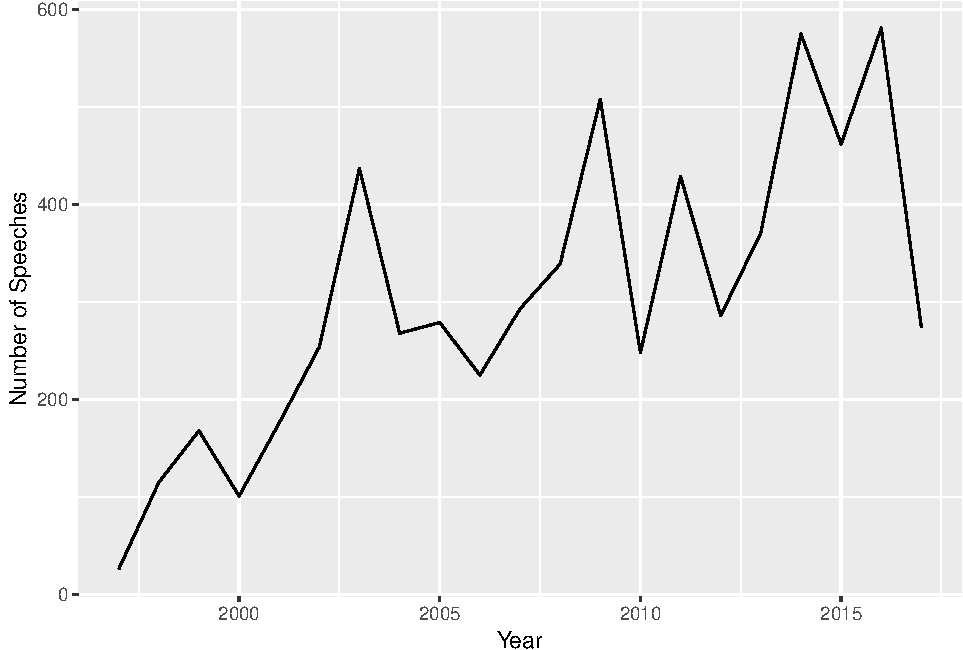
\includegraphics{methodology_files/figure-latex/middle-east-plot-1.pdf}
\caption{\label{fig:middle-east-plot}Number of Speeches in ``Middle East''
Topic per Year}
\end{figure}

\begin{figure}
\centering
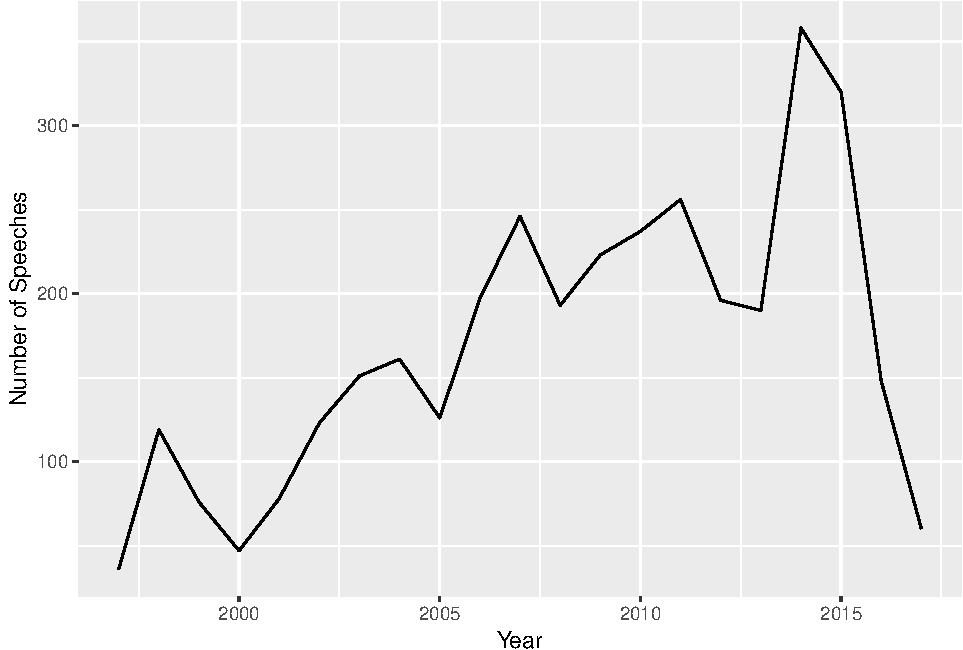
\includegraphics{methodology_files/figure-latex/wales-scotland-plot-1.pdf}
\caption{\label{fig:wales-scotland-plot}Number of Speeches in ``Wales \&
Scotland'' Topic per Year}
\end{figure}

\begin{figure}
\centering
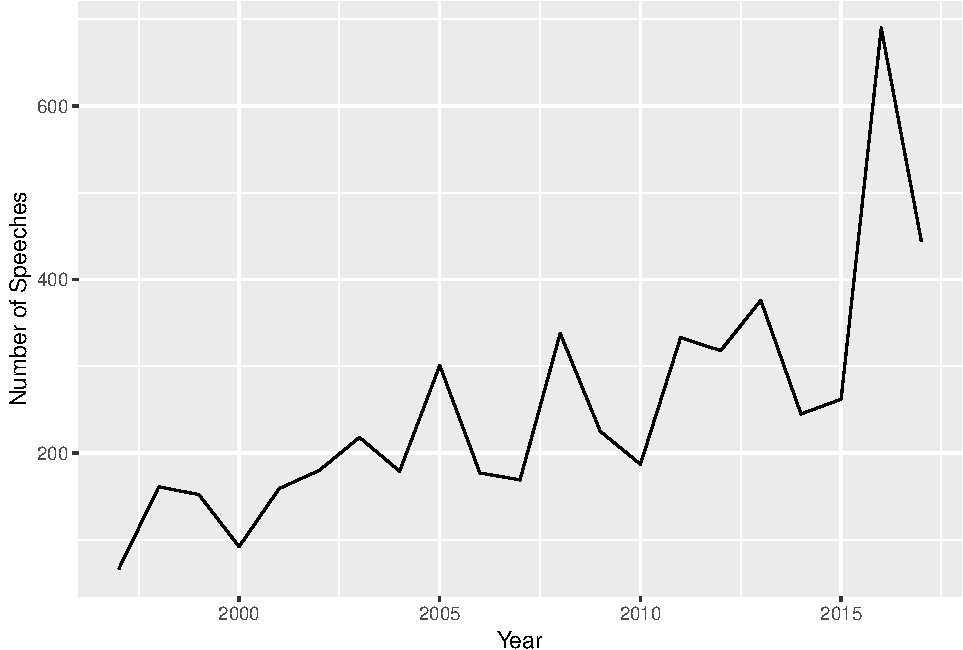
\includegraphics{methodology_files/figure-latex/eu-plot-1.pdf}
\caption{\label{fig:eu-plot}Number of Speeches in ``European Union'' Topic
per Year}
\end{figure}

\hypertarget{differences-between-male-aws-and-non-aws-labour-mps}{%
\subsection{Differences between Male, AWS and non-AWS Labour
MPs}\label{differences-between-male-aws-and-non-aws-labour-mps}}

From Table \ref{tab:estimate-table-k0} we can see the relationship
between the frequency of topics among AWS, non-AWS and male Labour MPs.

There are 11 topics where the frequency AWS MPs is significantly
different from male MPs, but where its frequency amongst non-AWS MPs is
not significantly different. They are topics 1, 6, 7, 8, 14, 17, 20, 26,
35, 36, 39. 5 topics are proportionally greater among AWS MPs (Topic 8,
Schools, Topic 14, Policy impact, Topic 26, Pensions, Topic 35, Alcohol
\& tobacco, Topic 36, Place names) and 6 topics are less common (Topic
1, Employment \& unions, Topic 6, Northern Ireland, Topic 7, Committee,
Topic 17, Communications, Topic 20, International development, Topic 39,
Private companies).

There are 7 topics where its proportion amongst non-AWS MPs is
significantly different from male MPs, but where its proportion amongst
AWS MPs is not significantly different. They are topics 5, 16, 24, 37,
44, 46, 57. 5 topics are proportionally greater among AWS MPs (Topic 16,
Regional development, Topic 37, Budget, Topic 44, Utilities \& PFI,
Topic 46, Local authorities, Topic 57, Locations) and 2 topics are less
common (Topic 5, Police, firefighters \& prison, Topic 24, Higher
education \& skills).

There is 1 topic (Topic 50, Questions) where there is no significant
difference in frequency among both AWS and non-AWS MPS, relative to male
Labour MPs.

There are 10 topics where AWS and non-AWS MPs differ significantly in
proportion from male Labour MPs, but are not both higher/lower than male
MPs. AWS MPs are significantly more likely to mention 5 topics (Topic
13, Ministers, Topic 22, Sport \& culture, Topic 38, Tax, Topic 49,
Transport, Topic 58, Jobs \& manufacturing) than male MPs, while non-AWS
mps are significantly less likely to mention those topics. The opposite
is true for the other 5 topics (Topic 2, Legal system, Topic 18,
Immigration, Topic 28, Issues, Topic 42, Bills, Topic 59, Small
business), which AWS MPs are significantly less likely and non-AWS MPs
are significantly more likely to mention than male Labour MPs.

However, an estimate being statistically significant -- i.e.~estimates
for AWS and non-AWS MPs where the \emph{p} value as reported in Table
\ref{tab:estimate-table-k0} is \textless{} 0.05 -- does not tell us
anything about the relative value of those frequency differences. For
example, in topic 21, Benefits and disability, frequency estimates for
both AWS and non-AWS MPs are significantly different (\emph{p}
\textless{} 0.05) from the frequency estimate for male Labour MPs.
However, while the frequency value for the benefits and disability topic
is 1.20\% for male MPs, and 1.30\% for non-AWS MPs, it is 2.41\% for AWS
MPs. Non-AWS Labour MPs are only slightly more likely to bring up
benefits and disability than male Labour MPs, while AWS MPs discuss it
almost twice as much as their male colleagues.

Figure \ref{fig:p-effect1} shows the frequency for the topics where AWS
and non-AWS MPs differ the most. Figure \ref{fig:p-effect2} shows the
frequency for the topics where AWS and non-AWS MPs are most similar to
each other, regardless of their similarity to male Labour MPs. Figure
\ref{fig:p-effect-cv} is the topics with the most variation, between
AWS, non-AWS and male Labour MPs. Figures \ref{fig:p-effect1},
\ref{fig:p-effect2} and \ref{fig:p-effect-cv} all use the coefficient of
variation to measure variance between each group of MPs. Figures
\ref{fig:p-effect1} and \ref{fig:p-effect2} only use female Labour MPS,
Figure \ref{fig:p-effect-cv} uses all three groups. Errors bars in all
three sets of figures are for 95\% confidence intervals.

\begin{figure}
\centering
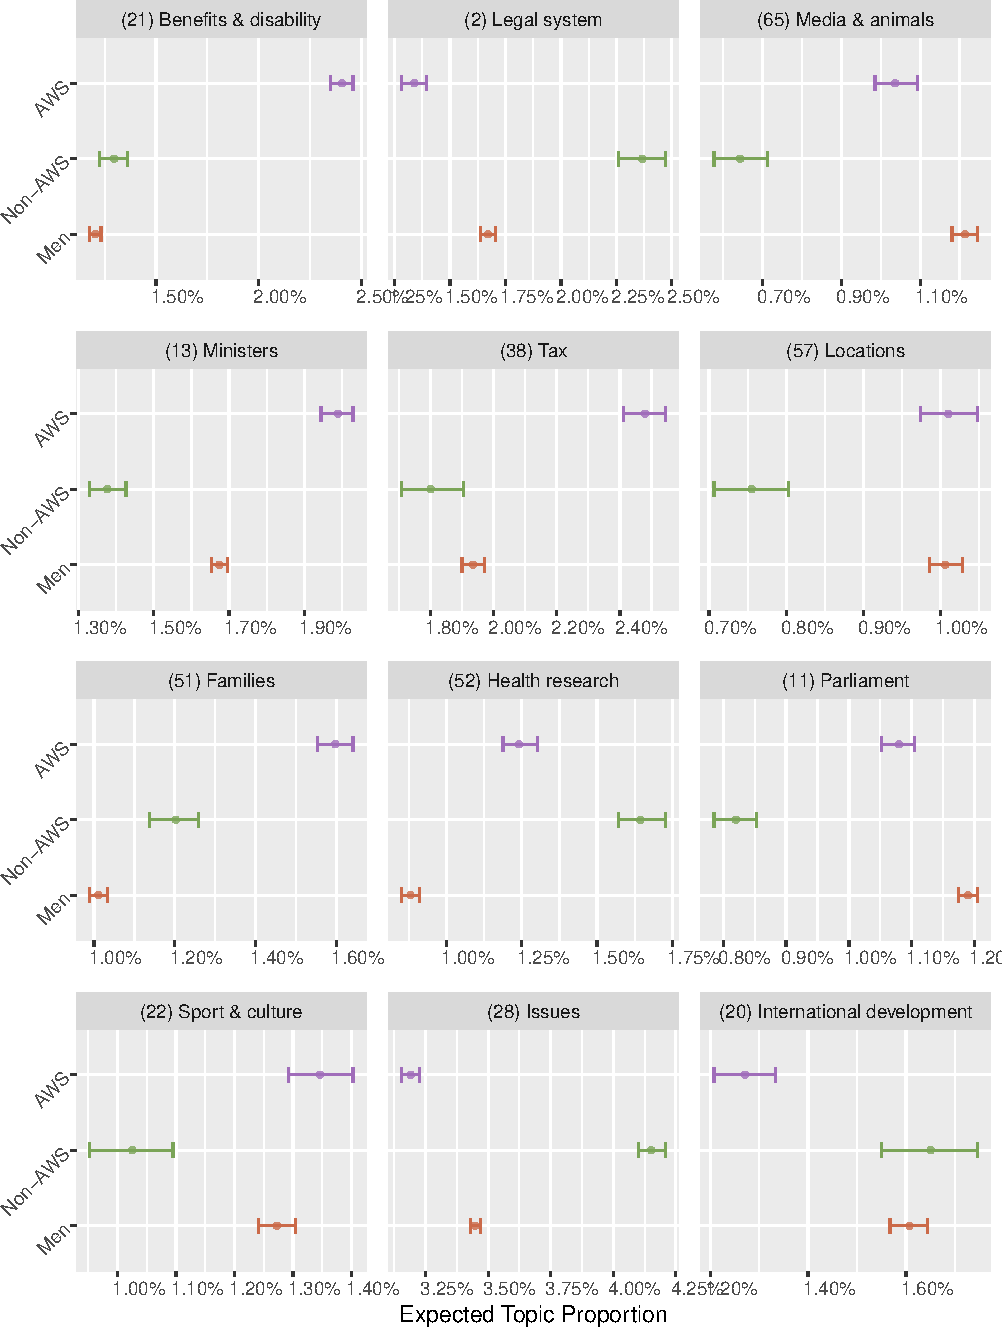
\includegraphics{methodology_files/figure-latex/p-effect1-1.pdf}
\caption{\label{fig:p-effect1}Where AWS MPs are most distinct from non-AWS
female MPs}
\end{figure}

\begin{figure}
\centering
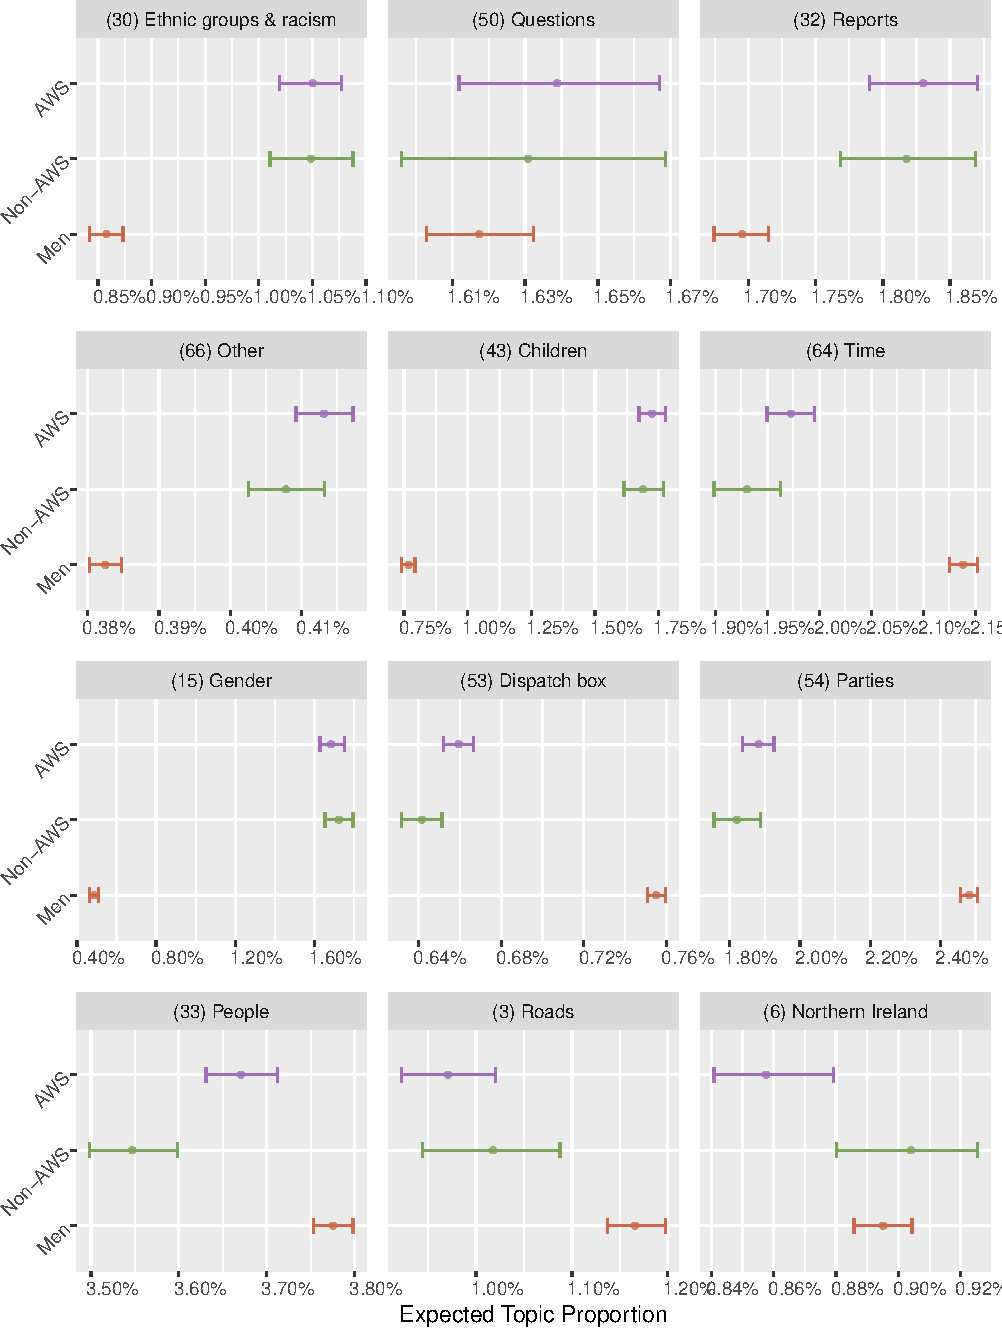
\includegraphics{methodology_files/figure-latex/p-effect2-1.pdf}
\caption{\label{fig:p-effect2}Where AWS MPs are most similar to non-AWS
female MPs}
\end{figure}

\begin{figure}
\centering
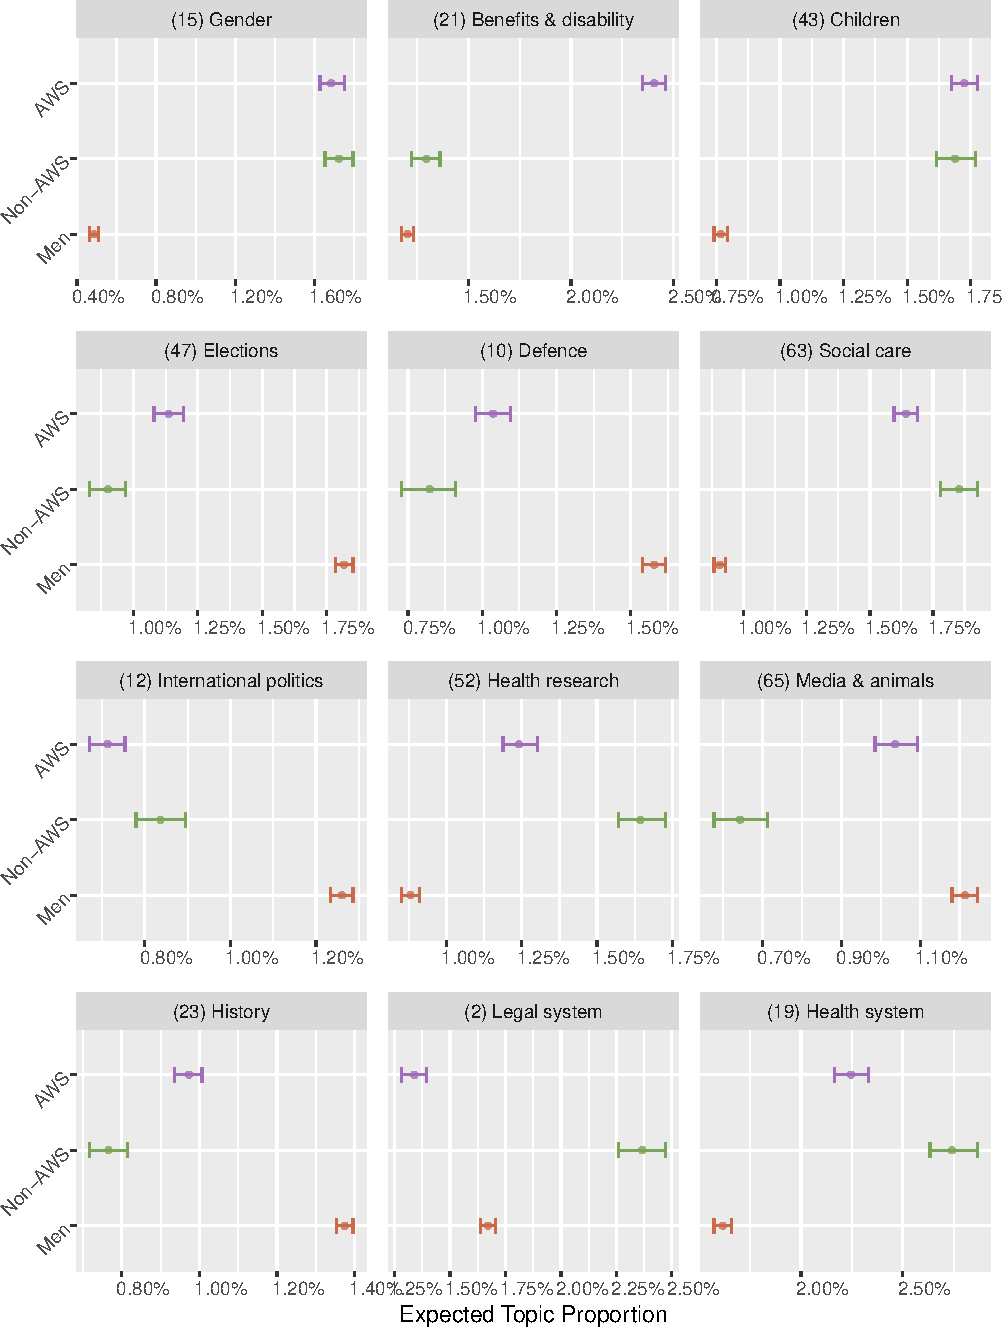
\includegraphics{methodology_files/figure-latex/p-effect-cv-1.pdf}
\caption{\label{fig:p-effect-cv}Topics with the greatest frequency
coefficient of variation}
\end{figure}

\hypertarget{discussion}{%
\section{Discussion}\label{discussion}}

There do not appear to be substantial or meaningful differences in the
speaking styles of female Labour MPs selected through all women
shortlists when compared to their female colleagues selected through
open shortlists using LIWC. This is possibly due to the speaking style
dominant in British parliamentary debate, which is more formal than the
speech used in most day-to-day conversation. LIWC was developed by
American researchers, and the LIWC dictionary may not be able to capture
stylistic differences between American and British English, and may not
include words commonly used in formal British English speech, limiting
its usefulness in the context of British political debate.

There is more distinction between AWS and non-AWS MPs in terms and
topics.
\protect\hyperlink{ux5cux2520Naiveux5cux2520Bayesux5cux2520classification}{Naive
Bayes classification} was able to accurately determine the AWS status of
female Labour MPs with slightly greater accuracy than it could
distinguish between male and female Labour MPs (71.22\% and 70.67\%,
respectively).

AWS MPs are far more likely to make reference to their constituency and
constituents. In the debate between whether MPs should be ``delegates''
or ``trustees'' -- the ``mandate-independence controversy'' outlined by
Pitkin (\protect\hyperlink{ref-pitkin1967}{1967}) -- the references to
their constituents and constituencies suggests AWS MPs shy away from the
Burkean concept of trusteeship and see themselves more as strict
representatives of their constituents. In Andeweg \& Thomassen's
(\protect\hyperlink{ref-andeweg2005}{2005}) typology of \emph{ex
ante}/\emph{ex post} and above/below political representation, AWS MPs
lean towards representation ``from below'', although their selection
process is \emph{ex ante}/\emph{ex post}. AWS MPs also use events and
individuals in their constituency as examples when speaking on a given
topic (see the
\protect\hyperlink{ux5cux2520AWSux5cux2520Referencesux5cux2520toux5cux2520Constituentsux5cux2520inux5cux2520Context}{Appendix}
for more examples).

AWS MPs refer to their constituents both specifically and in the
abstract, particularly when criticising government policy. For example,
in debate on 4th March 2015, Gemma Doyle, than the Labour MP for West
Dunbartonshire (elected on an AWS in 2010), when asked if she would give
way to Conservative MP Stephen Mosley, responded:

\begin{quote}
No, I will not {[}give way{]}, because my constituents want me to make
these points, not to give more time to Conservative Members.
\end{quote}

On 2nd June 2010, during debate on Israel-Palestine, Valerie Vaz, MP for
Walsall South, also used the views of her constituents to support her
position:

\begin{quote}
My constituents want more than pressure. Will the Foreign Secretary come
back to the House and report on a timetable for the discussions on a
diplomatic solution, just as we did on Ireland?
\end{quote}

On 4th April 2001, Betty Williams, member for Conwy from 1997--2010,
raised the case of a wilderness guide in her constituency unable to
access parts of the countryside due to foot and mouth disease:

\begin{quote}
Is my right hon. Friend aware that there is continuing concern about the
limited access to the countryside and crags of north Wales? May I draw
his attention to the circumstances of my constituent, Ric Potter? Like
many others, he has had to travel to Scotland, where there is greater
access. Will my right hon. Friend help us to enable people such as Ric
Potter to find work in outdoor pursuits?
\end{quote}

\clearpage

\hypertarget{appendix}{%
\section{Appendix}\label{appendix}}

\hypertarget{gender-effect-estimates}{%
\subsection{Gender effect estimates}\label{gender-effect-estimates}}

Estimate effects of different topics, using only gender (Table
\ref{tab:estimate-table-gender}).

\begin{longtabu} to \linewidth {>{\raggedright}X>{\raggedleft}X>{\raggedleft}X>{\raggedleft}X>{\raggedleft}X>{\raggedright}X}
\caption{\label{tab:estimate-table-gender}Topic Estimates}\\
\toprule
 &  & Estimate & Standard Error & t value & Pr(>|t|)\\
\midrule
\endfirsthead
\caption[]{\label{tab:estimate-table-gender}Topic Estimates \textit{(continued)}}\\
\toprule
 &  & Estimate & Standard Error & t value & Pr(>|t|)\\
\midrule
\endhead
\
\endfoot
\bottomrule
\endlastfoot
 & Intercept & 0.0120561 & 0.0001233 & 97.7458509 & < 0.001 ***\\
\cmidrule{2-6}
\multirow{-2}{*}{\raggedright\arraybackslash (1) Employment \& unions} & Female & -0.0009786 & 0.0002204 & -4.4396315 & < 0.001 ***\\
\cmidrule{1-6}
 & Intercept & 0.0167102 & 0.0001677 & 99.6358100 & < 0.001 ***\\
\cmidrule{2-6}
\multirow{-2}{*}{\raggedright\arraybackslash (2) Legal system} & Female & 0.0001861 & 0.0002867 & 0.6492618 & 0.52\\
\cmidrule{1-6}
 & Intercept & 0.0116864 & 0.0001469 & 79.5274864 & < 0.001 ***\\
\cmidrule{2-6}
\multirow{-2}{*}{\raggedright\arraybackslash (3) Roads} & Female & -0.0018110 & 0.0002574 & -7.0349793 & < 0.001 ***\\
\cmidrule{1-6}
 & Intercept & 0.0112593 & 0.0001746 & 64.4711132 & < 0.001 ***\\
\cmidrule{2-6}
\multirow{-2}{*}{\raggedright\arraybackslash (4) Housing} & Female & 0.0054870 & 0.0002870 & 19.1204992 & < 0.001 ***\\
\cmidrule{1-6}
 & Intercept & 0.0140238 & 0.0001747 & 80.2546259 & < 0.001 ***\\
\cmidrule{2-6}
\multirow{-2}{*}{\raggedright\arraybackslash (5) Police, firefighters \& prison} & Female & 0.0008970 & 0.0002998 & 2.9917221 & 0.003 **\\
\cmidrule{1-6}
 & Intercept & 0.0089592 & 0.0000450 & 198.8903532 & < 0.001 ***\\
\cmidrule{2-6}
\multirow{-2}{*}{\raggedright\arraybackslash (6) Northern Ireland} & Female & -0.0002231 & 0.0000821 & -2.7163043 & 0.007 **\\
\cmidrule{1-6}
 & Intercept & 0.0213132 & 0.0001509 & 141.2139750 & < 0.001 ***\\
\cmidrule{2-6}
\multirow{-2}{*}{\raggedright\arraybackslash (7) Committee} & Female & -0.0015245 & 0.0002307 & -6.6073185 & < 0.001 ***\\
\cmidrule{1-6}
 & Intercept & 0.0147366 & 0.0001975 & 74.6029960 & < 0.001 ***\\
\cmidrule{2-6}
\multirow{-2}{*}{\raggedright\arraybackslash (8) Schools} & Female & 0.0009898 & 0.0003519 & 2.8128100 & 0.005 **\\
\cmidrule{1-6}
 & Intercept & 0.0170286 & 0.0002027 & 84.0111642 & < 0.001 ***\\
\cmidrule{2-6}
\multirow{-2}{*}{\raggedright\arraybackslash (9) Energy \& climate change} & Female & -0.0026669 & 0.0003638 & -7.3306532 & < 0.001 ***\\
\cmidrule{1-6}
 & Intercept & 0.0157819 & 0.0001837 & 85.9128350 & < 0.001 ***\\
\cmidrule{2-6}
\multirow{-2}{*}{\raggedright\arraybackslash (10) Defence} & Female & -0.0061172 & 0.0003240 & -18.8794191 & < 0.001 ***\\
\cmidrule{1-6}
 & Intercept & 0.0119042 & 0.0000790 & 150.6173576 & < 0.001 ***\\
\cmidrule{2-6}
\multirow{-2}{*}{\raggedright\arraybackslash (11) Parliament} & Female & -0.0019543 & 0.0001429 & -13.6787831 & < 0.001 ***\\
\cmidrule{1-6}
 & Intercept & 0.0125948 & 0.0001249 & 100.8499998 & < 0.001 ***\\
\cmidrule{2-6}
\multirow{-2}{*}{\raggedright\arraybackslash (12) International politics} & Female & -0.0050786 & 0.0002170 & -23.4024173 & < 0.001 ***\\
\cmidrule{1-6}
 & Intercept & 0.0167087 & 0.0001064 & 157.0415815 & < 0.001 ***\\
\cmidrule{2-6}
\multirow{-2}{*}{\raggedright\arraybackslash (13) Ministers} & Female & 0.0011454 & 0.0001923 & 5.9551523 & < 0.001 ***\\
\cmidrule{1-6}
 & Intercept & 0.0115397 & 0.0000460 & 251.1090985 & < 0.001 ***\\
\cmidrule{2-6}
\multirow{-2}{*}{\raggedright\arraybackslash (14) Policy impact} & Female & 0.0009556 & 0.0000875 & 10.9167682 & < 0.001 ***\\
\cmidrule{1-6}
 & Intercept & 0.0048738 & 0.0001146 & 42.5372998 & < 0.001 ***\\
\cmidrule{2-6}
\multirow{-2}{*}{\raggedright\arraybackslash (15) Gender} & Female & 0.0121863 & 0.0002379 & 51.2176906 & < 0.001 ***\\
\cmidrule{1-6}
 & Intercept & 0.0230313 & 0.0001276 & 180.4911579 & < 0.001 ***\\
\cmidrule{2-6}
\multirow{-2}{*}{\raggedright\arraybackslash (16) Regional development} & Female & 0.0026193 & 0.0002503 & 10.4645867 & < 0.001 ***\\
\cmidrule{1-6}
 & Intercept & 0.0097462 & 0.0001202 & 81.0915937 & < 0.001 ***\\
\cmidrule{2-6}
\multirow{-2}{*}{\raggedright\arraybackslash (17) Communications} & Female & -0.0009899 & 0.0002069 & -4.7848162 & < 0.001 ***\\
\cmidrule{1-6}
 & Intercept & 0.0087105 & 0.0000900 & 96.8147319 & < 0.001 ***\\
\cmidrule{2-6}
\multirow{-2}{*}{\raggedright\arraybackslash (18) Immigration} & Female & -0.0000391 & 0.0001635 & -0.2394474 & 0.81\\
\cmidrule{1-6}
 & Intercept & 0.0161788 & 0.0001976 & 81.8627819 & < 0.001 ***\\
\cmidrule{2-6}
\multirow{-2}{*}{\raggedright\arraybackslash (19) Health system} & Female & 0.0079743 & 0.0003600 & 22.1488945 & < 0.001 ***\\
\cmidrule{1-6}
 & Intercept & 0.0160465 & 0.0001897 & 84.5865773 & < 0.001 ***\\
\cmidrule{2-6}
\multirow{-2}{*}{\raggedright\arraybackslash (20) International development} & Female & -0.0020679 & 0.0003358 & -6.1579789 & < 0.001 ***\\
\cmidrule{1-6}
 & Intercept & 0.0120722 & 0.0001441 & 83.8028248 & < 0.001 ***\\
\cmidrule{2-6}
\multirow{-2}{*}{\raggedright\arraybackslash (21) Benefits \& disability} & Female & 0.0080944 & 0.0002832 & 28.5770350 & < 0.001 ***\\
\cmidrule{1-6}
 & Intercept & 0.0127412 & 0.0001526 & 83.4724542 & < 0.001 ***\\
\cmidrule{2-6}
\multirow{-2}{*}{\raggedright\arraybackslash (22) Sport \& culture} & Female & -0.0003753 & 0.0002649 & -1.4166824 & 0.16\\
\cmidrule{1-6}
 & Intercept & 0.0137581 & 0.0001117 & 123.2082084 & < 0.001 ***\\
\cmidrule{2-6}
\multirow{-2}{*}{\raggedright\arraybackslash (23) History} & Female & -0.0046801 & 0.0001833 & -25.5317143 & < 0.001 ***\\
\cmidrule{1-6}
 & Intercept & 0.0143325 & 0.0001641 & 87.3629912 & < 0.001 ***\\
\cmidrule{2-6}
\multirow{-2}{*}{\raggedright\arraybackslash (24) Higher education \& skills} & Female & -0.0004494 & 0.0003006 & -1.4950418 & 0.13\\
\cmidrule{1-6}
 & Intercept & 0.0155213 & 0.0000474 & 327.6313660 & < 0.001 ***\\
\cmidrule{2-6}
\multirow{-2}{*}{\raggedright\arraybackslash (25) Concurring point} & Female & -0.0026315 & 0.0000760 & -34.6035104 & < 0.001 ***\\
\cmidrule{1-6}
 & Intercept & 0.0147019 & 0.0001709 & 86.0482540 & < 0.001 ***\\
\cmidrule{2-6}
\multirow{-2}{*}{\raggedright\arraybackslash (26) Pensions} & Female & 0.0019874 & 0.0002808 & 7.0777074 & < 0.001 ***\\
\cmidrule{1-6}
 & Intercept & 0.0177894 & 0.0001316 & 135.2139528 & < 0.001 ***\\
\cmidrule{2-6}
\multirow{-2}{*}{\raggedright\arraybackslash (27) Points of order} & Female & -0.0054025 & 0.0002166 & -24.9447457 & < 0.001 ***\\
\cmidrule{1-6}
 & Intercept & 0.0345025 & 0.0000980 & 352.1646087 & < 0.001 ***\\
\cmidrule{2-6}
\multirow{-2}{*}{\raggedright\arraybackslash (28) Issues} & Female & 0.0006780 & 0.0001716 & 3.9511379 & < 0.001 ***\\
\cmidrule{1-6}
 & Intercept & 0.0131800 & 0.0000540 & 244.1589822 & < 0.001 ***\\
\cmidrule{2-6}
\multirow{-2}{*}{\raggedright\arraybackslash (29) Constituencies} & Female & 0.0023276 & 0.0001069 & 21.7824341 & < 0.001 ***\\
\cmidrule{1-6}
 & Intercept & 0.0085781 & 0.0000728 & 117.8578866 & < 0.001 ***\\
\cmidrule{2-6}
\multirow{-2}{*}{\raggedright\arraybackslash (30) Ethnic groups \& racism} & Female & 0.0019552 & 0.0001365 & 14.3196680 & < 0.001 ***\\
\cmidrule{1-6}
 & Intercept & 0.0150304 & 0.0001578 & 95.2713075 & < 0.001 ***\\
\cmidrule{2-6}
\multirow{-2}{*}{\raggedright\arraybackslash (31) Amendments} & Female & -0.0028669 & 0.0002705 & -10.5980156 & < 0.001 ***\\
\cmidrule{1-6}
 & Intercept & 0.0169724 & 0.0001117 & 151.9867135 & < 0.001 ***\\
\cmidrule{2-6}
\multirow{-2}{*}{\raggedright\arraybackslash (32) Reports} & Female & 0.0012779 & 0.0001865 & 6.8516021 & < 0.001 ***\\
\cmidrule{1-6}
 & Intercept & 0.0377446 & 0.0001213 & 311.2792086 & < 0.001 ***\\
\cmidrule{2-6}
\multirow{-2}{*}{\raggedright\arraybackslash (33) People} & Female & -0.0014521 & 0.0002123 & -6.8400753 & < 0.001 ***\\
\cmidrule{1-6}
 & Intercept & 0.0135410 & 0.0001549 & 87.4194387 & < 0.001 ***\\
\cmidrule{2-6}
\multirow{-2}{*}{\raggedright\arraybackslash (34) Wales \& Scotland} & Female & -0.0031743 & 0.0002506 & -12.6669967 & < 0.001 ***\\
\cmidrule{1-6}
 & Intercept & 0.0108579 & 0.0001486 & 73.0683773 & < 0.001 ***\\
\cmidrule{2-6}
\multirow{-2}{*}{\raggedright\arraybackslash (35) Alcohol \& tobacco} & Female & 0.0005320 & 0.0002832 & 1.8786468 & 0.060\\
\cmidrule{1-6}
 & Intercept & 0.0083659 & 0.0000671 & 124.6776088 & < 0.001 ***\\
\cmidrule{2-6}
\multirow{-2}{*}{\raggedright\arraybackslash (36) Place names} & Female & 0.0007972 & 0.0001241 & 6.4237856 & < 0.001 ***\\
\cmidrule{1-6}
 & Intercept & 0.0246505 & 0.0001775 & 138.8996009 & < 0.001 ***\\
\cmidrule{2-6}
\multirow{-2}{*}{\raggedright\arraybackslash (37) Budget} & Female & -0.0003435 & 0.0002961 & -1.1599722 & 0.25\\
\cmidrule{1-6}
 & Intercept & 0.0193082 & 0.0001896 & 101.8596764 & < 0.001 ***\\
\cmidrule{2-6}
\multirow{-2}{*}{\raggedright\arraybackslash (38) Tax} & Female & 0.0030544 & 0.0003310 & 9.2272811 & < 0.001 ***\\
\cmidrule{1-6}
 & Intercept & 0.0123871 & 0.0001199 & 103.3046194 & < 0.001 ***\\
\cmidrule{2-6}
\multirow{-2}{*}{\raggedright\arraybackslash (39) Private companies} & Female & -0.0009559 & 0.0002220 & -4.3062780 & < 0.001 ***\\
\cmidrule{1-6}
 & Intercept & 0.0094757 & 0.0001428 & 66.3605526 & < 0.001 ***\\
\cmidrule{2-6}
\multirow{-2}{*}{\raggedright\arraybackslash (40) Environment \& fishing} & Female & -0.0024801 & 0.0002435 & -10.1854049 & < 0.001 ***\\
\cmidrule{1-6}
 & Intercept & 0.0141387 & 0.0001700 & 83.1774783 & < 0.001 ***\\
\cmidrule{2-6}
\multirow{-2}{*}{\raggedright\arraybackslash (41) Crime} & Female & 0.0052430 & 0.0003115 & 16.8290865 & < 0.001 ***\\
\cmidrule{1-6}
 & Intercept & 0.0244386 & 0.0001508 & 162.0410131 & < 0.001 ***\\
\cmidrule{2-6}
\multirow{-2}{*}{\raggedright\arraybackslash (42) Bills} & Female & -0.0012130 & 0.0002557 & -4.7439287 & < 0.001 ***\\
\cmidrule{1-6}
 & Intercept & 0.0076822 & 0.0001213 & 63.3511535 & < 0.001 ***\\
\cmidrule{2-6}
\multirow{-2}{*}{\raggedright\arraybackslash (43) Children} & Female & 0.0094502 & 0.0002461 & 38.3935766 & < 0.001 ***\\
\cmidrule{1-6}
 & Intercept & 0.0123659 & 0.0000838 & 147.6006401 & < 0.001 ***\\
\cmidrule{2-6}
\multirow{-2}{*}{\raggedright\arraybackslash (44) Utilities \& PFI} & Female & -0.0001325 & 0.0001597 & -0.8294008 & 0.41\\
\cmidrule{1-6}
 & Intercept & 0.0174606 & 0.0002080 & 83.9606437 & < 0.001 ***\\
\cmidrule{2-6}
\multirow{-2}{*}{\raggedright\arraybackslash (45) Middle East} & Female & -0.0020795 & 0.0003607 & -5.7649929 & < 0.001 ***\\
\cmidrule{1-6}
 & Intercept & 0.0179838 & 0.0001437 & 125.1849736 & < 0.001 ***\\
\cmidrule{2-6}
\multirow{-2}{*}{\raggedright\arraybackslash (46) Local authorities} & Female & 0.0015586 & 0.0002836 & 5.4965933 & < 0.001 ***\\
\cmidrule{1-6}
 & Intercept & 0.0181834 & 0.0001549 & 117.3877176 & < 0.001 ***\\
\cmidrule{2-6}
\multirow{-2}{*}{\raggedright\arraybackslash (47) Elections} & Female & -0.0075879 & 0.0002715 & -27.9430467 & < 0.001 ***\\
\cmidrule{1-6}
 & Intercept & 0.0180191 & 0.0000681 & 264.6774024 & < 0.001 ***\\
\cmidrule{2-6}
\multirow{-2}{*}{\raggedright\arraybackslash (48) Debate} & Female & -0.0018256 & 0.0001238 & -14.7506463 & < 0.001 ***\\
\cmidrule{1-6}
 & Intercept & 0.0163759 & 0.0001857 & 88.1991855 & < 0.001 ***\\
\cmidrule{2-6}
\multirow{-2}{*}{\raggedright\arraybackslash (49) Transport} & Female & -0.0002969 & 0.0003477 & -0.8538425 & 0.39\\
\cmidrule{1-6}
 & Intercept & 0.0161647 & 0.0000757 & 213.4856091 & < 0.001 ***\\
\cmidrule{2-6}
\multirow{-2}{*}{\raggedright\arraybackslash (50) Questions} & Female & 0.0001682 & 0.0001301 & 1.2927442 & 0.20\\
\cmidrule{1-6}
 & Intercept & 0.0101120 & 0.0001164 & 86.8890866 & < 0.001 ***\\
\cmidrule{2-6}
\multirow{-2}{*}{\raggedright\arraybackslash (51) Families} & Female & 0.0044922 & 0.0002501 & 17.9608814 & < 0.001 ***\\
\cmidrule{1-6}
 & Intercept & 0.0087873 & 0.0001603 & 54.8116345 & < 0.001 ***\\
\cmidrule{2-6}
\multirow{-2}{*}{\raggedright\arraybackslash (52) Health research} & Female & 0.0050129 & 0.0002923 & 17.1518648 & < 0.001 ***\\
\cmidrule{1-6}
 & Intercept & 0.0075482 & 0.0000252 & 299.9335737 & < 0.001 ***\\
\cmidrule{2-6}
\multirow{-2}{*}{\raggedright\arraybackslash (53) Dispatch box} & Female & -0.0010058 & 0.0000411 & -24.4759297 & < 0.001 ***\\
\cmidrule{1-6}
 & Intercept & 0.0248257 & 0.0001495 & 166.0099980 & < 0.001 ***\\
\cmidrule{2-6}
\multirow{-2}{*}{\raggedright\arraybackslash (54) Parties} & Female & -0.0062183 & 0.0002451 & -25.3739370 & < 0.001 ***\\
\cmidrule{1-6}
 & Intercept & 0.0211074 & 0.0000674 & 313.1127111 & < 0.001 ***\\
\cmidrule{2-6}
\multirow{-2}{*}{\raggedright\arraybackslash (55) Statements} & Female & -0.0025215 & 0.0001226 & -20.5654157 & < 0.001 ***\\
\cmidrule{1-6}
 & Intercept & 0.0163664 & 0.0001702 & 96.1683285 & < 0.001 ***\\
\cmidrule{2-6}
\multirow{-2}{*}{\raggedright\arraybackslash (56) European Union} & Female & -0.0044278 & 0.0002939 & -15.0664007 & < 0.001 ***\\
\cmidrule{1-6}
 & Intercept & 0.0100682 & 0.0001051 & 95.7956424 & < 0.001 ***\\
\cmidrule{2-6}
\multirow{-2}{*}{\raggedright\arraybackslash (57) Locations} & Female & -0.0008438 & 0.0001896 & -4.4503909 & < 0.001 ***\\
\cmidrule{1-6}
 & Intercept & 0.0176030 & 0.0001701 & 103.4783706 & < 0.001 ***\\
\cmidrule{2-6}
\multirow{-2}{*}{\raggedright\arraybackslash (58) Jobs \& manufacturing} & Female & 0.0002215 & 0.0003125 & 0.7086483 & 0.48\\
\cmidrule{1-6}
 & Intercept & 0.0070547 & 0.0000690 & 102.2200613 & < 0.001 ***\\
\cmidrule{2-6}
\multirow{-2}{*}{\raggedright\arraybackslash (59) Small business} & Female & -0.0000227 & 0.0001167 & -0.1948699 & 0.85\\
\cmidrule{1-6}
 & Intercept & 0.0328354 & 0.0001082 & 303.3701317 & < 0.001 ***\\
\cmidrule{2-6}
\multirow{-2}{*}{\raggedright\arraybackslash (60) Agreement \& disagreement} & Female & -0.0102158 & 0.0001823 & -56.0338702 & < 0.001 ***\\
\cmidrule{1-6}
 & Intercept & 0.0187326 & 0.0001134 & 165.1455528 & < 0.001 ***\\
\cmidrule{2-6}
\multirow{-2}{*}{\raggedright\arraybackslash (61) Voluntary sector} & Female & 0.0075517 & 0.0002253 & 33.5146669 & < 0.001 ***\\
\cmidrule{1-6}
 & Intercept & 0.0152785 & 0.0000587 & 260.3794919 & < 0.001 ***\\
\cmidrule{2-6}
\multirow{-2}{*}{\raggedright\arraybackslash (62) Comments} & Female & -0.0036504 & 0.0000997 & -36.6196859 & < 0.001 ***\\
\cmidrule{1-6}
 & Intercept & 0.0090888 & 0.0001324 & 68.6336761 & < 0.001 ***\\
\cmidrule{2-6}
\multirow{-2}{*}{\raggedright\arraybackslash (63) Social care} & Female & 0.0080677 & 0.0002317 & 34.8179514 & < 0.001 ***\\
\cmidrule{1-6}
 & Intercept & 0.0213910 & 0.0000681 & 314.0303987 & < 0.001 ***\\
\cmidrule{2-6}
\multirow{-2}{*}{\raggedright\arraybackslash (64) Time} & Female & -0.0017923 & 0.0001249 & -14.3468017 & < 0.001 ***\\
\cmidrule{1-6}
 & Intercept & 0.0121571 & 0.0001637 & 74.2672732 & < 0.001 ***\\
\cmidrule{2-6}
\multirow{-2}{*}{\raggedright\arraybackslash (65) Media \& animals} & Female & -0.0030953 & 0.0002716 & -11.3961506 & < 0.001 ***\\
\cmidrule{1-6}
 & Intercept & 0.0038287 & 0.0000119 & 322.4905663 & < 0.001 ***\\
\cmidrule{2-6}
\multirow{-2}{*}{\raggedright\arraybackslash (66) Other} & Female & 0.0002877 & 0.0000200 & 14.3849523 & < 0.001 ***\\*
\end{longtabu}

\hypertarget{closeness-in-frequency-for-each-topic}{%
\subsection{Closeness in frequency for each
topic}\label{closeness-in-frequency-for-each-topic}}

Using the frequency of a topic among male MPs as a baseline, there are
35 topics where the frequency among AWS MPs is proportionally closer, in
absolute terms, than the frequency of the topic among female MPs. The
inverse is true for the remaining 31 topics.

Relative to each other, there are 34 topics where the frequency between
AWS and non-AWS MPs are closer to each other than either is to the topic
frequency in male MPs. In 18 topics, the frequency between AWS and male
MPs are the most similar, and in the remaining 14 topics the difference
in frequency are smallest between non-AWS and male MPs. See Table
\ref{tab:absolute-differences} for details.

\begin{longtabu} to \linewidth {>{\raggedright}X>{\raggedright}X>{\raggedright\arraybackslash}p{6cm}}
\caption{\label{tab:absolute-differences}Absolute Differences}\\
\toprule
Topic & Women Relative to Male MPs & Most Similar\\
\midrule
\endfirsthead
\caption[]{\label{tab:absolute-differences}Absolute Differences \textit{(continued)}}\\
\toprule
Topic & Women Relative to Male MPs & Most Similar\\
\midrule
\endhead
\
\endfoot
\bottomrule
\endlastfoot
(1) Employment \& unions & Non-AWS more like male & Non-AWS more like male\\
(2) Legal system & AWS more like male & AWS more like male\\
(3) Roads & Non-AWS more like male & Women more similar to each other\\
(4) Housing & Non-AWS more like male & Women more similar to each other\\
(5) Police, firefighters \& prison & AWS more like male & AWS more like male\\
\addlinespace
(6) Northern Ireland & Non-AWS more like male & Non-AWS more like male\\
(7) Committee & Non-AWS more like male & Women more similar to each other\\
(8) Schools & Non-AWS more like male & Non-AWS more like male\\
(9) Energy \& climate change & Non-AWS more like male & Women more similar to each other\\
(10) Defence & AWS more like male & Women more similar to each other\\
\addlinespace
(11) Parliament & AWS more like male & AWS more like male\\
(12) International politics & Non-AWS more like male & Women more similar to each other\\
(13) Ministers & Non-AWS more like male & Non-AWS more like male\\
(14) Policy impact & Non-AWS more like male & Non-AWS more like male\\
(15) Gender & AWS more like male & Women more similar to each other\\
\addlinespace
(16) Regional development & AWS more like male & AWS more like male\\
(17) Communications & Non-AWS more like male & Women more similar to each other\\
(18) Immigration & AWS more like male & AWS more like male\\
(19) Health system & AWS more like male & Women more similar to each other\\
(20) International development & Non-AWS more like male & Non-AWS more like male\\
\addlinespace
(21) Benefits \& disability & Non-AWS more like male & Non-AWS more like male\\
(22) Sport \& culture & AWS more like male & AWS more like male\\
(23) History & AWS more like male & Women more similar to each other\\
(24) Higher education \& skills & AWS more like male & AWS more like male\\
(25) Concurring point & Non-AWS more like male & Women more similar to each other\\
\addlinespace
(26) Pensions & Non-AWS more like male & Non-AWS more like male\\
(27) Points of order & AWS more like male & Women more similar to each other\\
(28) Issues & AWS more like male & AWS more like male\\
(29) Constituencies & Non-AWS more like male & Women more similar to each other\\
(30) Ethnic groups \& racism & Non-AWS more like male & Women more similar to each other\\
\addlinespace
(31) Amendments & Non-AWS more like male & Women more similar to each other\\
(32) Reports & Non-AWS more like male & Women more similar to each other\\
(33) People & AWS more like male & Women more similar to each other\\
(34) Wales \& Scotland & AWS more like male & Women more similar to each other\\
(35) Alcohol \& tobacco & Non-AWS more like male & Non-AWS more like male\\
\addlinespace
(36) Place names & Non-AWS more like male & Non-AWS more like male\\
(37) Budget & AWS more like male & AWS more like male\\
(38) Tax & Non-AWS more like male & Non-AWS more like male\\
(39) Private companies & Non-AWS more like male & Non-AWS more like male\\
(40) Environment \& fishing & AWS more like male & Women more similar to each other\\
\addlinespace
(41) Crime & AWS more like male & Women more similar to each other\\
(42) Bills & Non-AWS more like male & Non-AWS more like male\\
(43) Children & Non-AWS more like male & Women more similar to each other\\
(44) Utilities \& PFI & AWS more like male & AWS more like male\\
(45) Middle East & AWS more like male & Women more similar to each other\\
\addlinespace
(46) Local authorities & AWS more like male & AWS more like male\\
(47) Elections & AWS more like male & Women more similar to each other\\
(48) Debate & AWS more like male & AWS more like male\\
(49) Transport & AWS more like male & AWS more like male\\
(50) Questions & Non-AWS more like male & Women more similar to each other\\
\addlinespace
(51) Families & Non-AWS more like male & Non-AWS more like male\\
(52) Health research & AWS more like male & Women more similar to each other\\
(53) Dispatch box & AWS more like male & Women more similar to each other\\
(54) Parties & AWS more like male & Women more similar to each other\\
(55) Statements & AWS more like male & AWS more like male\\
\addlinespace
(56) European Union & Non-AWS more like male & Women more similar to each other\\
(57) Locations & AWS more like male & AWS more like male\\
(58) Jobs \& manufacturing & AWS more like male & AWS more like male\\
(59) Small business & AWS more like male & AWS more like male\\
(60) Agreement \& disagreement & Non-AWS more like male & Women more similar to each other\\
\addlinespace
(61) Voluntary sector & AWS more like male & Women more similar to each other\\
(62) Comments & Non-AWS more like male & Women more similar to each other\\
(63) Social care & AWS more like male & Women more similar to each other\\
(64) Time & AWS more like male & Women more similar to each other\\
(65) Media \& animals & AWS more like male & AWS more like male\\
(66) Other & Non-AWS more like male & Women more similar to each other\\*
\end{longtabu}

\hypertarget{theta-distribution}{%
\subsection{\texorpdfstring{\(\theta\)
distribution}{\textbackslash{}theta distribution}}\label{theta-distribution}}

Figure \ref{fig:theta-boxplot} shows the distribution of \(\theta\)
scores used to assign overall topics to individual speeches in Table
\ref{tab:topic-summary-table}, per topic.

\begin{figure}
\centering
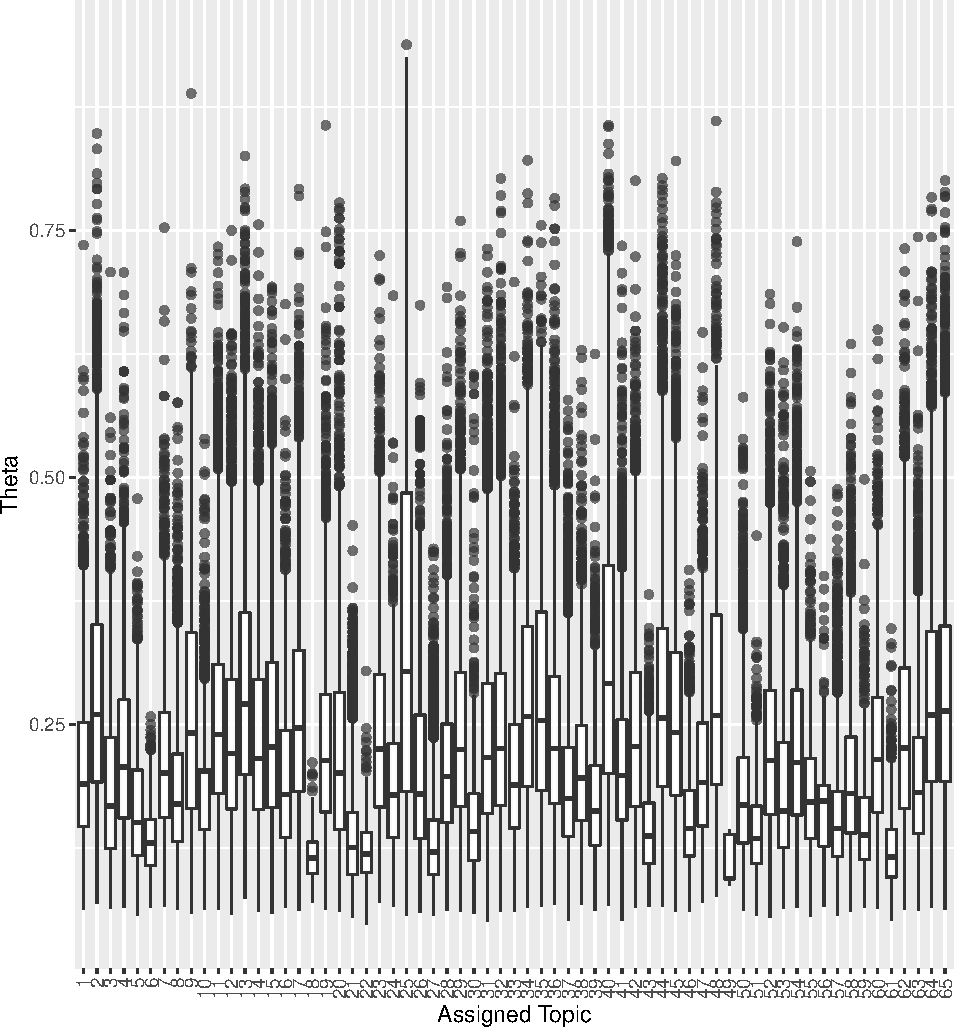
\includegraphics{methodology_files/figure-latex/theta-boxplot-1.pdf}
\caption{\label{fig:theta-boxplot}Theta Values in Topic Assignment}
\end{figure}

\hypertarget{aws-references-to-constituents-in-context}{%
\subsection{AWS References to Constituents in
Context}\label{aws-references-to-constituents-in-context}}

A random selection of 2\% of all references to ``my constituency'', ``my
constituent'' and ``my constituents'', by AWS MPs, in context.

\begin{longtabu} to \linewidth {>{\raggedright}X>{\raggedright}X>{\raggedright}X}
\caption{\label{tab:constituent-kwic}A random sample of KWIC's}\\
\toprule
Pre & Keyword & Post\\
\midrule
\endfirsthead
\caption[]{\label{tab:constituent-kwic}A random sample of KWIC's \textit{(continued)}}\\
\toprule
Pre & Keyword & Post\\
\midrule
\endhead
\
\endfoot
\bottomrule
\endlastfoot
. I was briefed by a vehicle hire company in & my constituency & called Reflex and, quite frankly, if such banking\\
150 per cent. two years ago. Another of & my constituents & has advised me of an application for an 85 per\\
already begun, for example just over the border from & my constituency & in the constituency of my hon. Friend the Member\\
in which Cornish children study. Three secondary schools in & my constituency & will be located on the same site, and one\\
Manchester has been doing a major infrastructure project, and & my constituents & are at the end of their tether about the lack\\
\addlinespace
patient at the BRI, and Airedale hospital is in & my constituency & . The hon. Member for South Cambridgeshire Mr.\\
, but the reality is there to be seen in & my constituency & . On Saturday I met a delegation of workers from\\
to use their abilities and develop their talents. In & my constituency & , 366 young people who have been unemployed for more\\
I believe that the most effective electoral registration officer in & my constituency & is mum. It is mum who fills in the\\
can arise from defective gas appliances, because two of & my constituents & , young students in their 20s, died from carbon\\
\addlinespace
£ 3.6 million. Some 9\% of people in & my constituency & are hard-working, entrepreneurial self-employed people, and today is\\
my right hon. Friend congratulate Aldercar community school in & my constituency & and its staff and pupils? The percentage of pupils\\
",  One particular concern for many of & my constituents & is bus fares. As I have said, my\\
,  Jobs and employment are the biggest issue in & my constituency & and the latest figures now show that just under 2,000\\
otherwise reach. The Psychiatric Rehabilitation Association is based in & my constituency & and was set up in 1959-it is no coincidence that\\
\addlinespace
financial inclusion fund. Where would the Minister suggest that & my constituents & who are struggling with debt and excessive and escalating charges\\
and without the full participation of the British people, & my constituents & and the country will never forgive them.\\
. There is an additional problem that is relevant to & my constituency & . It contains a large outdoor venue called the National\\
if they continue to propose new services that, in & my constituents & ' view, favour the administration of the hospital or\\
in red tape. That will be a turn-off. & My constituency & and the town in which it is situated has a\\
\addlinespace
With my right hon. Friend's local knowledge of & my constituency & , she will know that many of my constituents are\\
", to close a wide range of services at & my constituency's & local hospital, St Helier. Most of the controversy\\
I am extremely worried for & my constituents & in Ashton-under-Lyne, Droylsden and Failsworth, and for people\\
One of the shortlisted sites is at Barnard Castle in & my constituency & , and that would produce 1,000 jobs.\\
making ends meet has been raised with me repeatedly by & my constituents & , including Graeme McGrory, who cares for his partner\\
\addlinespace
One piece of transport infrastructure that & my constituency & and that of the hon. Member for Buckingham John\\
A director of Sirus Automotive who lives in & my constituency & would like to take on apprentices, but he has\\
" Three people who know that better than most are & my constituents & Mark, Joanne and Ben King. In 2011,\\
There are 3,540 women affected by the changes in & my constituency & . Does my hon. Friend agree that the 1995\\
have been down in the detail of rail provision in & my constituency & , but these are important matters for many of those\\
\addlinespace
just a few examples of the work being done in & my constituency & . I recently had the privilege of accompanying the Gateshead\\
, but that does not help the large number of & my constituents & who have lost some, if not all, of\\
was the only mainstream candidate in the general election in & my constituency & who did not have their picture taken while pointing to\\
was not even in the mortgage application, NatWest told & my constituents & that it was in the process of adding it.\\
is a measure of the Government's achievement that people in & my constituency & and elsewhere in Northamptonshire can look forward to a secure\\
\addlinespace
clothing company announced the closure of two more factories in & my constituency & and the neighbouring Erewash constituency. A huge number of\\
my primary care trust in north-east Derbyshire and dentists in & my constituency & to find a local solution. These reforms coincide with\\
Cross, just a few miles up the road from & my constituency & . That pipe manufacturing works has been taken over by\\
go ahead. There is huge concern about this in & my constituency & and across the north. Was the Prime Minister told\\
backgrounds, including poor backgrounds, and is representative of & my constituency & . That is the sort of school that Labour Members\\
\addlinespace
are subject to a TPIM. This information would let & my constituents & know whether potential terrorism suspects had returned to London.\\
. Gentleman for his generosity. Is he aware that & my constituency & is probably the one with the highest number of gas\\
because I have had direct experience of the issue in & my constituency & . A woman came over here as the wife of\\
. Let us take the feed-in tariff fiasco. In & my constituency & alone, we are losing many jobs, because a\\
What practical advice can the Secretary of State give to & my constituents & , as some 3,000 householders in my constituency face a\\
\addlinespace
sport, that this is good enough for kids in & my constituency & ?\\
a fair deal on jobs, getting young people in & my constituency & and others involved in working our way out of the\\
argument is best explained by reference to the case of & my constituent & , Neil Kenny, who raised his concerns about the\\
to LEAs give rise to some questions, including in & my constituency & from Unison, which is concerned that LEAs might use\\
Such travel will be available to all 17,600 pensioners in & my constituency & . ,  In February I visited\\
\addlinespace
",  What point is there in forcing & my constituent & who is a single dad who has his two children\\
replies, perhaps he can respond to the questions that & my constituent & has raised. What is she to do? She\\
ask my hon. Friend to offer an undertaking to & my constituents & in Mitcham and Morden that an option appraisal of intermediate\\
he would be interested to hear the Minister's response to & my constituent & Maureen Davenport. The Minister said that the maximum state\\
in child benefit, which will help 13,800 families in & my constituency & . My real reason for tabling the question is to\\
\addlinespace
Finchley and Golders Green Mike Freer), many of & my constituents & killed by lorries have died at junctions, including some\\
Hall the plight of former United Engineering Forgings workers in & my constituency & who will not receive the returns from their final salary\\
London has had Oyster cards for nine years, but & my constituents & are still waiting. Although Transport for Greater Manchester is\\
again have a university. However, Nene college in & my constituency & hopes to change all that, and I support strongly\\
Enforcement Campaign-in Cardiff, and particularly to the work of & my constituent & , Professor John Shepherd, who works in the dental\\
\addlinespace
and assets than non-disabled people. In London, where & my constituency & and the constituency of my hon. Friend the Member\\
in particular from the circumstances of students in Northampton. & My constituency & contains both a higher education and a further education college\\
the marine Bill on the grounds of its irrelevance to & my constituents & , because, like the hon. Lady, I\\
deepest concern for the families involved, especially given that & my constituency & neighbours that of my hon. Friend the Member for\\
services can expand on the slow line so that all & my constituents & benefit from the west coast main line upgrade?\\
\addlinespace
rehabilitation. ,  The people of & my constituency & have been horrified by those cases, and it is\\
Labour Government we have achieved a tremendous amount. In & my constituency & the number of people claiming jobseeker's allowance has almost halved\\
they complain? Where will the local accountability go? & My constituents & very much value the highly accessible local service that they\\
",  Since helping the Jarrow marchers, & my constituency & has continued to welcome people from throughout the UK,\\
and not-for-profit groups, of which there are many in & my constituency & , doing immensely valuable work. They all too often\\
\addlinespace
as soon as possible. Indeed, for some of & my constituents & , reform is already coming too late.\\
bus travel in Wales. I have met pensioners in & my constituency & who say that it has transformed their lives. As\\
and Sir Malcolm Thornton. All have represented part of & my constituency & and all left this House on 20 April or 1\\
Ports is the operator at the port of Immingham in & my constituency & . The companies there firmly believe that they have paid\\
Conservative-controlled Bradford city council excluded the wonderful Ilkley lido in & my constituency & from the free swimming initiative for young people and pensioners\\
\addlinespace
for my hon. Friend's reply, and many of & my constituents & who have come across the benefit integrity project will be\\
Tero was not properly treated and offer the apology that & my constituent & deserves.\\
about their corporate social responsibilities. For the sake of & my constituents & in Mitcham, Morden and Colliers Wood who want something\\
change in the law. Regrettably, not only in & my constituency & but in many northern towns and cities, I see\\
on an issue that has been of great concern to & my constituents & . While I appreciate the cross-party consensus that exists on\\
\addlinespace
In & my constituency & of West Lancashire, the national lottery has supported 266\\
to meet the skills gap in engineering and construction in & my constituency & . ,  When I talk to\\
sat with the parents of the two children who were & my constituents & , as has Ken Livingstone, who made a private\\
who have been strongly encouraged to save The consultation in & my constituency & on the pensioners tax credit was extremely successful. The\\
Government for investing in the city of Bradford, helping & my constituents & to realise their potential. But in reality little has\\
\addlinespace
visited Dot To Dot, a community arts project in & my constituency & . It has a good record of involving the community\\
one regret the fact that Westminster, which covers half & my constituency & , has so far concentrated CCTV bids-I am sure with\\
also significant gaps in the Bill. One example from & my constituency & concerns a community hydro project in Saddleworth that might not\\
hon. Friend for that reply, but most of & my constituents & probably do not know what a low carbon transition plan\\
has provided opportunities where there were none before. In & my constituency & , there have been far more opportunities in the past\\
\addlinespace
to find examples of such practices. Another case in & my constituency & , with which I am dealing, involves elderly victims\\
. ,  The credit union in & my constituency & is fragile, because it serves an area in which\\
certainly applies to me because the acute trust that covers & my constituents & , who desperately need care, has the mother and\\
reveal a trend, and I see it happening in & my constituency & . It is a demonstrable fact that the polarisation between\\
 & My constituent & , John Warren, has specifically asked me to raise\\
\addlinespace
,  Bridges Project in Musselburgh in & my constituency & does a brilliant job in supporting young people. A\\
Spowart, a small firm of legal aid solicitors in & my constituency & . Solicitors at the firm are paid generally between £\\
, both as a national concern and as it affects & my constituency & . I am grateful to my hon. Friend for\\
, nor, sadly, are far too many of & my constituents & .\\
 & My constituents & in Hull are baffled by the Government's approach. At\\
\addlinespace
issue and go after these criminals who are preying on & my constituents & ?\\
even begin for another 12 months. Young people in & my constituency & should not have to spend another year on the dole\\
with the nutrition they need outside term time. In & my constituency & , several schools run summer programmes funded through the pupil\\
takes umbrage at being forced to do repairs-as some of & my constituents & , sadly, know to their cost.\\
",  I recently visited a care home in & my constituency & that is provided by a small charity and is rated\\
\addlinespace
House and members of the armed forces, such as & my constituent & , 19-year-old Private James Kenny of C company, 3rd\\
as out to Kent. There are seven stations in & my constituency & : Hither Green, Blackheath, Lee, Grove Park\\
Can my right hon. Friend give any assurance to & my constituent & , Mr. Peter Dyson, who has written to\\
Commons Library to conduct an analysis of the impact in & my constituency & . I discovered that 4,300 women and 3,800 men would\\
100 days of the new Parliament? Many businesses in & my constituency & are struggling significantly and would undoubtedly welcome a period of\\
\addlinespace
in 1992, as the Member for Woolwich, before & my constituency & was formed for the 1997 election. John Austin is\\
were building up and seemed to take action only once & my constituents & had suffered a very high level of nuisance and there\\
that further education institutions, such as Blackburn College in & my constituency & , will not receive a real-terms funding cut as a\\
",  On a more serious note, & my constituency & is home to manufacturers varying from Corus to Cadbury,\\
costs and cuts to working tax credits, families in & my constituency & will be worse off. I will not vote in\\
\addlinespace
be warm. It paid for basics like that in & my constituency & . I will not revisit the pain of tuition fees\\
is a national issue. The 900 steel workers in & my constituency & whose jobs are on the line expect him to guarantee\\
to begin by speaking about the NHS as experienced by & my constituents & . Getting an appointment to see a GP can be\\
I was struck by what one of & my constituents & said last weekend, which was that the attacks that\\
",  On 18 February, Llandudno in & my constituency & hosted the first North Wales criminal justice board conference.\\
\addlinespace
my hon. Friend foresee for the young people in & my constituency & if they are to suffer possible cuts alongside that idiosyncratic\\
busways and widen the M1. Is he aware that & my constituency & will have the new Translink guided busway by 2008 due\\
" Last week, I hosted a jobs fair in & my constituency & , as have many hon. Members on both sides\\
in the south-east will be dealt with in Parliament? & My constituents & want to know where we are going and what the\\
him to visit the brand-new children's centre in Elland in & my constituency & , which is due to open in January, and\\
\addlinespace
realities for people affected by this situation. One of & my constituents & is stuck out in Saudi Arabia. His work has\\
the past few days. When the problems started in & my constituency & on Monday night, we saw copycat criminality, mindless\\
those branches, in Catford and Blackheath, are in & my constituency & and two others, in Lewisham and Greenwich, are\\
 & My constituent & , Richard Belmar, has now spent nearly three years\\
Postwatch because I am unhappy about the consultation process in & my constituency & . I fully accept many of my hon. Friend's\\
\addlinespace
area of Keighley last Friday and talking to many of & my constituents & and taking on board many of their anxieties. On\\
of the major issues raised with me by carers in & my constituency & . We must take such issues on board.\textbackslash{}\\
that the voucher company Farepak, which is based in & my constituency & , collapsed this week, robbing thousands of people on\\
scientific reports recommend restricted phone use by younger children. & My constituents & do not believe that such recommendations tally with the telecommunications\\
. Mullin). This is a big issue in & my constituency & , where inappropriate development on garden sites is taking place\\
\addlinespace
scrutiny process, but it is impossible for me, & my constituents & or councillors of any party not involved in that enterprise\\
",  At the time, I was consulting & my constituents & about their attitudes to crime and antisocial behaviour, and\\
you prove it?  , & My constituency & is served by two hospitals: Dewsbury and District hospital\\
\% reduction. What reassurances can the Minister give to & my constituents & and firefighters that those latest cuts will not jeopardise or\\
. ,  Horwich visiting service in & my constituency & has lost funding and can no longer employ its part-time\\
\addlinespace
I have spoken to many businesses in & my constituency & . Will the hon. Gentleman concede that the Government's\\
prevent businesses from going into administration, as many in & my constituency & are likely to do. Finally, the local authority\\
I do not know whether my experience in & my constituency & has been exactly the same as that of my right\\
? ,  Many SMEs operate in & my constituency & , and I want to ensure that the skills base\\
that population live in Salford, the local authority for & my constituency & . ,  In last year's debate\\
\addlinespace
It is an issue that has been simmering away in & my constituency & and recently the rumours have turned to reality as the\\
of the parenting lessons that go on in schools in & my constituency & to great effect. The hon. Gentleman ignores those\\
a distraught couple who run a hedgehog rescue centre in & my constituency & . They are currently nursing back to health a hedgehog\\
people to think that that was the total sum of & my constituency & . It is an extremely nice place to spend Christmas\\
transparency about the impact. , & My constituents & are also anxious about the Government's proposals to allow fracking\\
\addlinespace
some of its provisions will have on vulnerable people in & my constituency & . ,  I shall first raise\\
key elements of creative business growth. Creative businesses in & my constituency & and in a large area to the west of London\\
In Pembrokeshire we have two oil refineries, one in & my constituency & . They were both affected by the blockades in September\\
thank the Minister for his reply. Head teachers in & my constituency & are concerned that Government have still not come forward with\\
the work of local authorities in my area. In & my constituency & , there are no high profile arts venues that hit\\
\addlinespace
many of the early asbestosis claims from Hebden Bridge in & my constituency & might not have succeeded under the proposed 75 per cent\\
job first.\textbackslash{}  , & My constituency & is pronounced\textbackslash{}  Erreywash\textbackslash{} , not\textbackslash{}\\
that is not regulated properly, with the result that & my constituents & , who have small sums of money available to invest\\
a picture of the winning design, but people in & my constituency & have seen many pictures before. I want work to\\
hour. I have written to all the headteachers in & my constituency & over the last few weeks, and they tell me\\
\addlinespace
this debate falls on an anniversary well worth remembering for & my constituents & . It is 20 years to the month that post-war\\
people of the east end, including the people of & my constituency & , talk to me about how excited they still are\\
I recently visited Bishop Barrington school in & my constituency & , which has got a new science lab and sports\\
the extent of the disruption and the problems caused for & my constituents & ? I would be happy to do that.\textbackslash{}\\
increase in the number of new homes being built in & my constituency & over the past 10 years or so. For the\\
\addlinespace
junior doctors who are the problem, but him? & My constituents-hundreds & of whom have written to me-overwhelmingly feel that he has\\
, ,  I do not think & my constituents & knew whether to laugh or cry.\\
about to be built in Walkden in the centre of & my constituency & . The new local improvement finance trust-LIFT-centre will include GP\\
is higher, and the dole queue is lengthening. & My constituents & are only too well aware of the exploitative practices of\\
" I am fortunate in having a research centre in & my constituency & at the university of Durham, which concentrates on enabling\\
\addlinespace
is talking about the wrong hospital, which many of & my constituents & will find most amusing.\\
of the Land Registry would be bad not just for & my constituents & but for the public as a whole. The revenue\\
The food banks in & my constituency & , which currently number at least six, tell me\\
of those issues. ,  In & my constituency & , the credit union benefits from capital and revenue from\\
children. I am indebted to a law company in & my constituency & called Just for Kids Law, which has raised with\\
\addlinespace
hope they are not giving false hope to many of & my constituents & . Will they just admit that they have made a\\
I have a range of energy-intensive industries in & my constituency & , including steel, glass, paper and the entire\\
the save Lewisham hospital campaign. But for now, & my constituents & still face the prospect of seriously downgraded services at their\\
from and bugbear for my constituents. On behalf of & my constituents & and their families, I very much look forward to\\
",  helped motorists and the hard-pressed hauliers in & my constituency-or & they could have looked at jobs for young people.\\
\addlinespace
Staff at Trinity, Bluecoat and Fernwood schools in & my constituency & are desperate for extra investment in their buildings. Will\\
The point about geography is critical in Cumbria, where & my constituency & is. Under the proposals, we will end up\\
will affect disabled youngsters. The What? centre in & my constituency & , which gives counselling to all youngsters, still does\\
closure of the offices is having a direct impact on & my constituency & . Walsall faces the closure of its HMRC office,\\
. ,  Frustration is evident among & my constituents & : for many years, they have felt marginalised and\\
\addlinespace
, larger numbers of people are choosing to live in & my constituency & but work in London. If we are to take\\
ethnic minority children, of whom there are many in & my constituency & . ,  We have dealt a\\
single parents in the country-I will return to that point-and & my constituents & think that the measure is unfair. How people in\\
should not come back from our holidays to find that & my constituents & , and those of my neighbours, have lost their\\
their area; I fully intend to do so in & my constituency & . ,  We also need better\\
\addlinespace
too much movement. I want Airedale general hospital in & my constituency & not just to survive, but to prosper. It\\
",  During the summer and autumn months, & my constituents & and those of many other hon. Members were affected\\
put a human face on many of the difficulties that & my constituents & experience. ,  In Newham,\\
Parent Action Network, which has its national headquarters in & my constituency & . It has just received nearly £ 400,000 in lottery\\
sector. On Friday, an independent community pharmacist in & my constituency & told me that he estimated that the Government cuts would\\
\addlinespace
it becomes an empty gesture. A community group in & my constituency & is setting up a community development trust, and it\\
since June and doubled since 2006. Young people in & my constituency & have been particularly badly hit, with a 288\%\\
police get back to strength to defend the people in & my constituency & of Mitcham and Morden?\\
to address have been influenced by what has happened in & my constituency & in the past 10 days as a series of incidents\\
, including those of Allied Steel and Wire's pensioners in & my constituency & ? They took the case to court through the unions\\
\addlinespace
Indeed, it is a stealth cut. In & my constituency & , the Tories will have to make stealth cuts such\\
communities across the UK. I understand the concerns of & my constituents & . I understand that when a family from a different\\
a vested interest in ensuring the safety and security of & my constituency & , which in the past has been a military target\\
infrastructure project is a massive economic opportunity for Wales and & my constituency & in particular. Will the Minister assure the House that\\
Nottingham that stands to lose most is the Meadows in & my constituency & . Before the last election, the Meadows, one\\
\addlinespace
am here this afternoon specifically to represent the concerns of & my constituents & who are trade union members in Parliament, as they\\
. Nothing could be further from the truth, as & my constituency & exemplifies. As I have already said, I represent\\
making are the very ones that have been made by & my constituents & , by the constituents of my hon. Friends and-I\\
, but wanted to take the opportunity to read out & my constituent's & comments so that Ministers understand the worry and concern.\\
firm of Hickman and Rose, which is based in & my constituency & ? She was due to speak at a conference organised\\
\addlinespace
Majesty's Opposition. That public money could be used for & my constituent & Grace Ryder, aged 9, who was recently diagnosed\\
changes that will affect 650 families and 1,500 children in & my constituency & . ,  These are ideologically driven\\
deal more about the birdlife in both estuaries that surround & my constituency & . ,  The Bill establishes a\\
 & My constituent & , the wonderful campaigner Marie Lyons, has doggedly pursued\\
\textbackslash{}  vote for their Muslim brother\textbackslash{} . & My constituents & were told that that was their religious duty. When\\
\addlinespace
. It will bring huge benefits to many families in & my constituency & who are on low or not very generous incomes.\\
anywhere. ,  The diversity of & my constituency & is one of the reasons why it is the best\\
c  The NHS in & my constituency & has moved beyond special measures into the success regime.\\
invited my right hon. and learned Friend to meet & my constituents & to hear what they think about our local NHS.\\
fleeing Ebola-affected countries are not left destitute and homeless? & My constituents & , Mr and Mrs Mahmood, have been working in\\
\addlinespace
pension credit, but I wondered whether Ministers could give & my constituent & and me advice on whether the notional sum tied up\\
first home. There are so many young people in & my constituency & who see homes priced out of their reach and for\\
There are also problems for low-income families, such as & my constituent & on Colleymoor Leys lane who says:\\
term. I know from the experience of businesses in & my constituency & and in the surrounding west midlands area that New Street\\
that he needs those, but he failed to tell & my constituents & watching yesterday that a 1p cut in duty will not\\
average, which show that over a fifth-22\% in & my constituency-of & people who resort to food banks for an emergency food\\*
\end{longtabu}

\hypertarget{references}{%
\section*{References}\label{references}}
\addcontentsline{toc}{section}{References}

\hypertarget{refs}{}
\leavevmode\hypertarget{ref-airoldi2016}{}%
Airoldi, E. M., \& Bischof, J. M. (2016). Improving and Evaluating Topic
Models and Other Models of Text. \emph{Journal of the American
Statistical Association}, \emph{111}(516), 1381--1403.
\url{https://doi.org/10.1080/01621459.2015.1051182}

\leavevmode\hypertarget{ref-andeweg2005}{}%
Andeweg, R. B., \& Thomassen, J. J. (2005). Modes of Political
Representation: Toward a New Typology. \emph{Legislative Studies
Quarterly}, \emph{30}(4), 507--528.
\url{https://doi.org/10.3162/036298005X201653}

\leavevmode\hypertarget{ref-arora2013}{}%
Arora, S., Ge, R., Halpern, Y., Mimno, D., Moitra, A., Sontag, D.,
\ldots{} Zhu, M. (2013). A Practical Algorithm for Topic Modeling with
Provable Guarantees. In S. Dasgupta \& D. McAllester (Eds.),
\emph{Proceedings of the 30th International Conference on Machine
Learning} (Vol. 28, pp. 280--288). Atlanta, Georgia, USA: PMLR.
Retrieved from \url{http://proceedings.mlr.press/v28/arora13.pdf}

\leavevmode\hypertarget{ref-audickas2017}{}%
Audickas, L., Hawkins, O., \& Cracknell, R. (2017). \emph{UK Election
Statistics: 1918-2017} (Briefing Paper No. CBP7529) (p. 89). London:
House of Commons Library. Retrieved from
\url{http://researchbriefings.parliament.uk/ResearchBriefing/Summary/CBP-7529}

\leavevmode\hypertarget{ref-benoit2018}{}%
Benoit, K. (2018). \emph{Quanteda: Quantitative Analysis of Textual
Data}. \url{https://doi.org/10.5281/zenodo.1004683}

\leavevmode\hypertarget{ref-benoit2018a}{}%
Benoit, K., \& Matsuo, A. (2018). \emph{Spacyr: Wrapper to the 'spaCy'
'NLP' Library}. Retrieved from \url{http://github.com/quanteda/spacyr}

\leavevmode\hypertarget{ref-blei2003}{}%
Blei, D. M., Ng, A. Y., \& Jordan, M. I. (2003). Latent Dirichlet
Allocation. \emph{Journal of Machine Learning Research}, \emph{3}(Jan),
993--1022.

\leavevmode\hypertarget{ref-bligh2010}{}%
Bligh, M., Merolla, J., Schroedel, J. R., \& Gonzalez, R. (2010).
Finding Her Voice: Hillary Clinton's Rhetoric in the 2008 Presidential
Campaign. \emph{Women's Studies}, \emph{39}(8), 823--850.
\url{https://doi.org/10.1080/00497878.2010.513316}

\leavevmode\hypertarget{ref-cohen1988}{}%
Cohen, J. (1988). \emph{Statistical power analysis for the behavioral
sciences} (2nd ed). Hillsdale, N.J: L. Erlbaum Associates.

\leavevmode\hypertarget{ref-fruchterman1991}{}%
Fruchterman, T. M. J., \& Reingold, E. M. (1991). Graph drawing by
force-directed placement. \emph{Software: Practice and Experience},
\emph{21}(11), 1129--1164. \url{https://doi.org/10.1002/spe.4380211102}

\leavevmode\hypertarget{ref-gagolewski2018}{}%
Gagolewski, M. (2018). R package stringi: Character string processing
facilities. \url{https://doi.org/10.5281/zenodo.1292492}

\leavevmode\hypertarget{ref-grimmer2013}{}%
Grimmer, J., \& Stewart, B. M. (2013). Text as Data: The Promise and
Pitfalls of Automatic Content Analysis Methods for Political Texts.
\emph{Political Analysis}, \emph{21}(03), 267--297.
\url{https://doi.org/10.1093/pan/mps028}

\leavevmode\hypertarget{ref-honnibal2017}{}%
Honnibal, M., \& Montani, I. (2017). spaCy 2: Natural language
understanding with Bloom embeddings, convolutional neural networks and
incremental parsing. \emph{To Appear}. Retrieved from
\url{https://spacy.io}

\leavevmode\hypertarget{ref-jones2016}{}%
Jones, J. J. (2016). Talk "Like a Man": The Linguistic Styles of Hillary
Clinton, 1992-2013. \emph{Perspectives on Politics}, \emph{14}(03),
625--642. \url{https://doi.org/10.1017/S1537592716001092}

\leavevmode\hypertarget{ref-kelly2016}{}%
Kelly, R., \& White, I. (2016). \emph{All-women shortlists} (Briefing
Paper No. 5057) (p. 34). London: House of Commons Library. Retrieved
from
\url{https://researchbriefings.parliament.uk/ResearchBriefing/Summary/SN05057}

\leavevmode\hypertarget{ref-kincaid1975}{}%
Kincaid, J. P., Fishburne, R. P., Rogers, R. L., \& Chissom, B. S.
(1975). \emph{Derivation of New Readability Formulas (Automated
Readability Index, Fog Count and Flesch Reading Ease Formula) for Navy
Enlisted Personnel:} Fort Belvoir, VA: Defense Technical Information
Center. \url{https://doi.org/10.21236/ADA006655}

\leavevmode\hypertarget{ref-lee2014c}{}%
Lee, M., \& Mimno, D. (2014). Low-dimensional Embeddings for
Interpretable Anchor-based Topic Inference. In \emph{Proceedings of the
2014 Conference on Empirical Methods in Natural Language Processing
(EMNLP)} (pp. 1319--1328). Doha, Qatar: Association for Computational
Linguistics. \url{https://doi.org/10.3115/v1/D14-1138}

\leavevmode\hypertarget{ref-mimno2011}{}%
Mimno, D., Wallach, H. M., Talley, E., Leenders, M., \& McCallum, A.
(2011). Optimizing semantic coherence in topic models. In
\emph{Proceedings of the 2011 Conference on Empirical Methods in Natural
Language Processing} (pp. 262--272). Edinburgh: Association for
Computational Linguistics. Retrieved from
\url{https://dl.acm.org/citation.cfm?id=2145432.2145462}

\leavevmode\hypertarget{ref-newman2008}{}%
Newman, M. L., Groom, C. J., Handelman, L. D., \& Pennebaker, J. W.
(2008). Gender Differences in Language Use: An Analysis of 14,000 Text
Samples. \emph{Discourse Processes}, \emph{45}(3), 211--236.
\url{https://doi.org/10.1080/01638530802073712}

\leavevmode\hypertarget{ref-odell2018}{}%
Odell, E. (2018). Hansard Speeches and Sentiment V2.5.1 {[}dataset{]}.
\url{https://doi.org/10.5281/zenodo.1306964}

\leavevmode\hypertarget{ref-pennebaker2015}{}%
Pennebaker, J. W., Boyd, R. L., Jordan, K., \& Blackburn, K. (2015). The
Development and Psychometric Properties of LIWC2015, 26. Retrieved from
\url{https://repositories.lib.utexas.edu/bitstream/handle/2152/31333/LIWC2015_LanguageManual.pdf}

\leavevmode\hypertarget{ref-pitkin1967}{}%
Pitkin, H. F. (1967). \emph{The concept of representation} (1. paperback
ed., {[}Nachdr.{]}). Berkeley, Calif.: Univ. of California Press.

\leavevmode\hypertarget{ref-quinn2010}{}%
Quinn, K. M., Monroe, B. L., Colaresi, M., Crespin, M. H., \& Radev, D.
R. (2010). How to Analyze Political Attention with Minimal Assumptions
and Costs. \emph{American Journal of Political Science}, \emph{54}(1),
209--228. \url{https://doi.org/10.1111/j.1540-5907.2009.00427.x}

\leavevmode\hypertarget{ref-roberts2016}{}%
Roberts, M. E., Stewart, B. M., \& Airoldi, E. M. (2016). A Model of
Text for Experimentation in the Social Sciences. \emph{Journal of the
American Statistical Association}, \emph{111}(515), 988--1003.
\url{https://doi.org/10.1080/01621459.2016.1141684}

\leavevmode\hypertarget{ref-roberts2018}{}%
Roberts, M. E., Stewart, B. M., \& Tingley, D. (2018). \emph{Stm: R
Package for Structural Topic Models}. Retrieved from
\url{http://www.structuraltopicmodel.com}

\leavevmode\hypertarget{ref-taddy2012}{}%
Taddy, M. A. (2012). On Estimation and Selection for Topic Models. In
\emph{Proceedings of the 15th International Conference on Artificial
Intelligence and Statistics} (Vol. 22, pp. 1184--1193). La Palma, Canary
Island: JMLR W\&CP.

\leavevmode\hypertarget{ref-yu2014}{}%
Yu, B. (2014). Language and gender in Congressional speech.
\emph{Literary and Linguistic Computing}, \emph{29}(1), 118--132.
\url{https://doi.org/10.1093/llc/fqs073}


\end{document}
